%\documentstyle[a4,twoside,epsf,makeidx]{sislman}
\documentclass[a4paper]{report}
\usepackage{sislman2}
\usepackage{graphicx}
\usepackage{fancyvrb}
\pagestyle{headings}
\usepackage{imakeidx} 
\makeindex
\begin{document}

\begin{titlepage}
  \vspace{5 cm}
  \begin{center}
  \Huge
  \textbf{SISL} \\
  \huge
  The SINTEF Spline Library \\ 
  \LARGE
  Reference Manual \\
  (version 4.7)\\ 
  \vspace{10 mm}
  \large
  SINTEF Digital, Mathematics and Cybernetics \\
  Mars 16, 2021
  \end{center}

\end{titlepage}

\pagenumbering{roman}
\tableofcontents
\cleardoublepage
\pagenumbering{arabic}
\setcounter{page}{1}
\chapter{Preface}
Welcome to the SISL 4.5 user's manual.  SISL stands for
\emph{\textbf{Si}ntef \textbf{S}pline \textbf{L}ibrary}, and has been gradually 
developed and enhanced for more than three decades by the geometry group at SINTEF in Oslo.
Although it is very comprehensive, its organisation is simple.  There are but a 
few structures, and its nearly four hundred main functions can usually be employed
directly and individually. This manual organises and explains the main routines.  However, much of this
information can also be found directly in the code in the form of commentaries.

The complete software package you have in your hands should contain the following:
\begin{itemize}
\item The SISL 4.5 distribution and reference guide (the document you are reading now)
\item Supplementary routines for writing SISL objects to streams (including file 
streams) in a simple ASCII format called \textbf{\Verb/Go/}.
\item A selection of \emph{sample programs}, designed to demonstrate functionalities
and use of SISL.
\item Source code for a simple \emph{viewer} that can be used to view geometric objects stored
in the \Verb/Go/-format.  This allows visual inspection of SISL-generated curves
and surfaces, as well as points.
\end{itemize}

\section{The structure of this document}
\textbf{Chapter 2} is a general introduction to SISL and its programming style. A simple example program
including instructions in how to compile and link the program and the expected output is provided.
Since it is strongly recommended that the user has some general knowledge of splines, this 
chapter also contains a couple of sections introducing the subject of spline curves and
surfaces. \\
\\
\textbf{Chapter 3 to 11} presents the main SISL routines.  \\
\\
\textbf{Chapter 12} goes through the provided sample programs and explain what these do,
and what the user can expect to learn from them.  There are a total of 15 sample 
programs, ranging from very basic to intermediate complexity.\\
\\
The goal of \textbf{Chapter 13} is to explain the use of the \emph{viewer program}, 
which is a small but handy tool for visually inspecting results from SISL routines.\\
\\
\textbf{Chapter 14} is an appendix presenting an explanation of the error codes used in SISL.\\
\\
Finally there is an \textbf{annex}, citing the text of the General Public License.

\section{The structure of the software package}\label{compile}
There are seven directories:
\begin{itemize}
\item \textbf{\Verb-include/-} - the inlude files related to the 4.5 release of SISL.
\item \textbf{\Verb-src/-} - the source code of the 4.5 release of SISL.
\item \textbf{\Verb-doc/-} - the basis for this document. 
\item \textbf{\Verb-streaming/-} - source code for the routines that can read and write
SISL objects to a stream.
\item \textbf{\Verb-examples/-} - sample programs making use of the SISL 4.5 source code.
\item \textbf{\Verb-viewer/-} - source code for a viewer that can be used to view SISL 
  objects saved in the \verb/Go/-format.
\item \textbf{\Verb-app/-} - the expected directory for test programs and applications. A
  couple of applications are provided including the example program described in Chapter 2.
\end{itemize}
Furthermore is the file CMakeLists.txt provided to facilitate building the library.

\section{Licensing information}
SISL is distributed under the \emph{GNU Affero General Public License} (aGPL).  The license text 
is given in its entirety as an annex to this document.  Commercial licenses are also
available from SINTEF.  You can contact Tor Dokken (tor.dokken@sintef.no) for more
information.

%% *what is included in this distibution
%% *explain chapters
%% *the manual
%% *licensing information
%% *compilation
%% *the object viewer

\chapter{General Introduction}
\label{introduction}
SISL is a geometric toolkit to model with curves and surfaces. It is a
library of C functions to perform operations such as the definition,
intersection and evaluation of NURBS (Non-Uniform Rational B-spline)
geometries. Since many applications use implicit geometric
representation such as planes, cylinders, tori etc., SISL can also
handle the interaction between such geometries and NURBS.

\medskip
Throughout this manual, a distinction is made between NURBS (the
default) and B-splines. The term B-splines is used for non-uniform
non-rational (or polynomial) B-splines. B-splines are used only where it
does not make sense to employ NURBS (such as the approximation of a
circle by a B-spline) or in cases where the research
community has yet to develop stable technology for treating NURBS.
A NURBS require more memory space than a B-spline, even when the
extra degrees of freedom in a NURBS are not used. Therefore the routines
are specified to give B-spline output whenever the extra degrees of
freedom are not required.

Transferring a B-spline into NURBS format is done by constructing a new
coefficient vector using the original B-spline coefficients and setting
all the rational weights equal to one (1).
This new coefficient vector is then given as input to the routine for
creating a new curve/surface object while specifying that the object to
be created should be of the NURBS (rational B-spline) type.

To approximate a NURBS by a B-spline, use the offset calculation
routines with an offset of zero.

The routines in SISL are designed to function on curves and surfaces
which are at least continuously differentiable. However many routines
will also handle continuous curves and surfaces, including piecewise
linear ones.

\medskip
All arrays in SISL are 1-dimensional. In an array with points or vertices
are the points stored consecutively. In a raster are points or vertices
stored consecutively while points in the first parameter direction have
the shortest stride (stored right after each other). There is a special
rule for vertices given as input to a rational curve or surface, see the
Sections~\ref{sec:newCurve} and~\ref{sec:newSurf}.

The three important data structures used by SISL are SISLCurve,
SISLSurf, and SISLIntcurve. These are defined in the Curve Utilities,
Surface Utilities, and Surface Interrogation modules respectively. Other
structures are SISLBox and SISLCone, which represents a bounding box and
a normal cone, respectively. It is
important to remember to always free these structures and also to free
internally allocated structures used to pass results to the application,
otherwise strange errors might result.

The various functions are equipped with a status variable, typically
placed as the last entity in the parameter list. It returns information
about whether or not the function succeeded in its purpose. A negative
value means failure, the result zero means success while a positive
number is a warning. Section~\ref{errorcodes} provides a list over
possible error messages where most occurances are explained. 

\medskip
SISL is divided into seven modules, partly in order to provide a logical
structure, but also to enable users with a specific application to use
subsets of SISL. There are three modules dealing with curves, three with
surfaces, and one module to perform data reduction on curves and
surfaces. The modules for
curves and surfaces focus on functions for creation and definition,
intersection and interrogation, and general utilities.

The chapters 3 to 11 in this manual contain information concerning the top
level functions of each module. Lower level functions not usually
required by an application are not included. Each top level function is
documented by describing the purpose, the input and output arguments and
an example of use. Input parameters specified in the examples are suggestions, the
actual values must be set dependent on context.
To get you started, this chapter contains an Example Program.

%\vfill
%\newpage

\section{\label{syntax}C Syntax Used in Manual}
This manual uses the K\&R style C syntax for historic reasons, but both
the ISO/ANSI and the K\&R C standards are supported by the library and
the include files.

\section{\label{dynamic}Dynamic Allocation in SISL}
In the description of all the functions in this manual, a
convention exists on when to declare or allocate arrays/objects outside a
function and when an array is allocated internally.
{\em NB! When memory for output arrays/objects are allocated inside a function you
must remember to free the allocated memory when it is not in use any
more.}

The convention is the following:
\begin{itemize}
\item If $[\,]$ is used in the synopsis and in the example it means
that the array has to be declared or allocated outside the function.
\item If $*$ is used it means that the function requires a
pointer and that the allocation will be done outside the function if necessary.
\item When either an array or an array of pointers or an object is to be
allocated in a function, two or three stars are used in the
synopsis.
To use the function you declare the parameter with one star less and use  \&
in the argument list.
\item For all output variables except arrays or objects
that are declared or allocated  outside the function you have to use \&
in the argument list.
\end{itemize}


\vfill
\newpage
\vfill
\newpage
\section{Creating the library}

In order to access SISL from your program you need one library inclusion, namely
the header file sisl.h. The statement
\begin{verbatim}
#include "sisl.h"
\end{verbatim}
must be written at the top of your main program.
In this header file all types
are defined.
It also contains all the
SISL top level function declarations.
Memory management and input/output require two more includes to avoid compiler warnings,
see Section~\ref{sec:exampleprog}.

SISL is prepared for makefile generation with CMake and equipped with a CMakeLists.txt file.
For information on using CMake, see www.cmake.org. The building procedure depends on whether your platform is
Linux or Windows.

\medskip
    {\noindent \bf LINUX}

Start by creating a build directory:
\begin{verbatim}
$ cd <path_to_source_code>
$ mkdir build
$ cd build
\end{verbatim}

Run the cmake program to setup the build process, selecting Debug or Release
as build type, optionally selecting a local install folder:
\begin{verbatim}
$ cmake .. -DCMAKE_BUILD_TYPE=Release (-DCMAKE_INSTALL_PREFIX=$HOME/install)
\end{verbatim}

For a gui-like cmake interface use ccmake (from cmake-ncurses-gui) or cmake-gui (from cmake.org).

Build the library:
\begin{verbatim}
$ make
\end{verbatim}
This will install the library in the build folder. Compilation and build of one particular
example program is done by a specific make statement:
\begin{verbatim}
$ make example01
\end{verbatim}
This option requires compilation of examples to be set in the Makefile.

Install the library to a local folder (requires the use of
-DCMAKE\_INSTALL\_PREFIX with a local folder in the previous step):
\begin{verbatim}
$ make install
\end{verbatim}

If the -DCMAKE\_INSTALL\_PREFIX in the cmake step was omitted or was set to a
system folder (like /usr/local) the user needs elevated privileges to install
the library:
\begin{verbatim}
$ sudo make install
\end{verbatim}

\medskip
{\noindent \bf Windows}

Add a new build folder somewhere. Start the CMake
executable and fill in the paths to the source and build folders. When
you run CMake, a Visual Studio project solution file will be generated
in the build folder.



\newpage
\section{An Example Program} \label{sec:exampleprog}

To clarify the previous section here is an example program designed to
test the SISL algorithm for intersecting a cone with
a B-spline curve. The program calls the SISL routines newCurve() documented in
Section ~\ref{sec:newCurve}, freeCurve() documented in~\ref{sec:freeCurve},
s1373() found in Section~\ref{sec:s1373} and freeIntcrvlist() in~\ref{sec:freeIntcrvlist}.

\begin{verbatim}
#include "sisl.h"
#include <stdlib.h>  
#include <stdio.h>

int main()
{
  SISLCurve *pc=0;                    /* Pointer to spline curve */
  double aepsco,aepsge;               /* Tolerances */
  double top[3],axispt[3],conept[3];  /* Representating the cone */
  double st[100],scoef[100];          /* Knot vector and coefficients of spline curve */
  double *spar;                       /* Parameter values of intersection points */
  int kstat;                          /* Return status from function calls */
  int cone_exists=0;
  int kk,kn,kdim;                     /* Order (polynomial degree+1), number of 
                                         coefficients and spatial dimension */
  int ki;                             /* Counter */
  int kpt,kcrv;                       /* Number of intersection points and curves */
  SISLIntcurve **qrcrv;               /* Array of pointer to intersection curves  */
  char ksvar[100];                    
  kdim=3;
  aepsge=0.001; /* Geometric tolerance */
  aepsco=0.000001; /* Computational tolerance. This parameter is included from 
                      historical reasons and no longer used */

  ksvar[0] = '0';  /* Arbitrary character */
  while (ksvar[0] != 'q')
    {
      printf("\n cu - define a new B-spline curve");
      printf("\n co - define a new cone");
      printf("\n i - intersect the B-spline curve with the cone");
      printf("\n q - quit");
      printf("\n> ");
      scanf("%s",ksvar);

      if (ksvar[0] == 'c' && ksvar[1] == 'u')
        {
          /* Define spline curve */
          printf("\n Give number of vertices, order of curve: ");
          scanf("%d %d", &kn, &kk);
          printf("Give knots values in ascending order: \n");
          for (ki=0; ki<kn+kk; ki++)
            {
               scanf("%lf",&st[ki]);
            }
          printf("Give vertices \n");
          for (ki=0; ki<kn*kdim; ki++)
            {
              scanf("%lf",&scoef[ki]);
            }
         if(pc) freeCurve(pc);

          /* Create curve */
          pc = newCurve(kn,kk,st,scoef,1,kdim,1);
        }
      else if (ksvar[0] == 'c' && ksvar[1] == 'o')
       {
         printf("\n Give top point: ");
         scanf("%lf %lf %lf",&top[0],&top[1],&top[2]);
         printf("\n Give a point on the axis: ");
         scanf("%lf %lf %lf",&axispt[0],&axispt[1],&axispt[2]);
         printf("\n Give a point on the cone surface: ");
         scanf("%lf %lf %lf",&conept[0],&conept[1],&conept[2]);
         cone_exists=1;
       }
      else if (ksvar[0] == 'i' && cone_exists && pc)
       {
         /* Intersect spline curve with cone */
         s1373(pc,top,axispt,conept,kdim,aepsco,aepsge,
               &kpt,&spar,&kcrv,&qrcrv,&kstat);
         printf("\n kstat %d",kstat);
         printf("\n kpt %d",kpt);
         printf("\n kcrv %d",kcrv);
         for (ki=0;ki<kpt;ki++)
          {
            printf("\nIntersection point %lf",spar[ki]);
          }
        if (spar)
          {
            /* The array containing parameter values of the intersection points between
               the curve and the cone is allocated inside s1373 and must be freed */
            free (spar);
            spar=0;
          }
        if (qrcrv)
         {
           /* The array containing pointers to intersection points curves between
              the curve and the cone is allocated inside s1373 and must be freed.
              This is done in a special function taking care of the intersection
              curves themselves */
          freeIntcrvlist(qrcrv,kcrv);
          qrcrv=0;
        }
      }
    }
  return 0;
}

\end{verbatim}
Note that sisl.h is included. stdlib.h is included to declare free, which
releases memory allocated in the function s1373. stdio.h declares printf and
scanf.

\bigskip

The program was compiled and built using the command:
\begin{verbatim}
$ make prog1
\end{verbatim}
Note that the program must be placed in the app folder and sisl\_COMPILE\_APPS must be set to true.

A sample run of prog1 went as follows:
\begin{verbatim}
$ prog1

     cu - define a new B-spline curve
     co - define a new cone
     i  - intersect the B-spline curve with the cone
     q  - quit
> cu

 Give number of vertices, order of curve: 2 2
Give knots values in ascending order:
0 0 1 1
Give vertices
1 0 0.5
-1 0 0.5

     cu - define a new B-spline curve
     co - define a new cone
     i  - intersect the B-spline curve with the cone
     q  - quit
> co

 Give top point: 0 0 1

 Give a point on the axis: 0 0 0

 Give a point on the cone surface: 1 0 0

     cu - define a new B-spline curve
     co - define a new cone
     i  - intersect the B-spline curve with the cone
     q  - quit
> i

 kstat 0
 kpt   2
 kcrv  0
Intersection point 0.250000
Intersection point 0.750000
     cu - define a new B-spline curve
     co - define a new cone
     i  - intersect the B-spline curve with the cone
     q  - quit
> q
$
\end{verbatim}
SISL found two intersection points given by the parameters
$0.25$ and $0.75$. These parameters correspond to the 3D points
$(-0.5,0,0.5)$ and $(0.5,0,0.5)$ (which could be found by calling
the evaluation routine s1221()). They lie on both
the B-spline curve and the cone --- as expected!

\section{B-spline Curves}

This section is optional reading for those who want to
become acquainted with some of the mathematics of
B-splines curves. For a description of the data structure for
B-spline curves in SISL, see section \ref{curveobject}.

A B-spline curve is defined by the formula
$$ {\bf c}(t) = \sum_{i=1}^{n} {\bf p}_{i} B_{i,k,{\bf t}}(t). $$
The dimension of the curve ${\bf c}$ is equal to that of its
{\it control points} ${\bf p}_i$. For example, if the dimension of the
control points
is one, the curve is a function, if the dimension is two,
the curve is planar, and if the dimension is three,
the curve is spatial. SISL also allows higher dimensions.

Thus, a B-spline curve is a linear combination of a sequence of B-splines
$B_{i,k,{\bf t}}$ (called a B-basis)
uniquely determined by a knot vector ${\bf t}$ and
the order $k$. Order is equivalent to polynomial degree plus one.
For example, if the order is two, the degree is one and the B-splines
and the curve $c$ they generate are (piecewise) linear.
If the order is three, the degree is two and the B-splines and
the curve are quadratic. Cubic B-splines and
curves have order 4 and degree 3, etc.

The parameter range of a B-spline curve ${\bf c}$ is the interval
$$ [t_k, t_{n+1}], $$
and so mathematically, the curve is a mapping
${\bf c}: [t_k, t_{n+1}] \to \RR^d$, where $d$ is the Euclidean space
dimension of its control points.

The complete representation of a B-spline curve consists of
\begin{description}
\item[$dim$]: The dimension of the underlying Euclidean space,
              $1,2,3,\ldots$.
\item[$n$]: The number of vertices (also the number of B-splines)
\item[$k$]: The order of the B-splines.
\item[${\bf t}$]: The knot vector of the B-splines.
            ${\bf t} = (t_1, t_2, \ldots, t_{n+k})$.
\item[${\bf p}$]: The control points of the B-spline curve.
           $p_{d,i}\;,\; d=1,\ldots,dim\;,\;
                i=1,\ldots,n.\;\;$
                e.g. when $dim = 3$, we have
                ${\bf p} = (x_1,y_1,z_1,x_2,y_2,z_2,\ldots,x_n,y_n,z_n)$.
\end{description}

We note that arrays in $c$ start at index 0 which means,
for example, that if the array $t$ holds the knot vector,
then $t[0] = t_1,\ldots, t[n+k-1] = t_{n+k}$
and the parameter interval goes from
$t[k-1]$ to $t[n]$. Similar considerations apply to the other arrays.

The data in the representation must satisfy certain conditions:
\begin{itemize}
\item The knot vector must be non-decreasing: $t_i \le t_{i+1}$.
      Moreover, two knots $t_i$ and $t_{i+k}$ must be distinct:
      $t_i < t_{i+k}$.
\item The number of vertices should be greater than or equal
      to the order of the curve: $n \ge k$.
\item There should be $k$ equal knots at the beginning and at the end
      of the knot vector; that is the knot vector ${\bf t}$
      must satisfy the conditions $t_1 = t_2 = \ldots = t_k$
      and $t_{n+1} = t_{n+2} = \ldots = t_{n + k}$.
\end{itemize}

To understand the representation better, we will look at
three parts of the
representation: the B-splines (the basis functions),
the knot vector and the control polygon.

\subsection{B-splines}

A set of B-splines is determined by the order $k$
and the knots. For example,
to define a single B-spline of degree one, we need three knots.
In figure~\ref{curve1} the three knots are marked as dots.
Knots can also be equal as shown in figure
\ref{curve2}.
By taking a linear combination of the three types of B-splines shown
in figures~\ref{curve1} and~\ref{curve2}
we can generate a linear spline function
as shown in figure~\ref{curve3}.
\begin{figure}
        \begin{center}
                \begin{picture}(250,80)(0,0)
                \put(80,0){\circle*{2}}
                \put(150,0){\circle*{2}}
                \put(230,0){\circle*{2}}

                \put(30,4){\vector(0,1){76}}
                \put(28,10){\line(1,0){4}}
                \put(28,70){\line(1,0){4}}
                \put(20,10){\makebox(0,0){0.0}}
                \put(20,70){\makebox(0,0){1.0}}

                \thicklines
                \put(80,10){\line(6,5){70}}
                \put(150,70){\line(4,-3){80}}
                \end{picture}\\
        \end{center}
  \caption{\label{curve1}A linear B-spline (order 2) defined by
                        three knots.}
\end{figure}
\begin{figure}
        \begin{center}
                \begin{picture}(300,85)(0,0)
                \put(40,0){\circle*{2}}
                \put(280,0){\circle*{2}}
                \put(120,5){\circle*{2}}
                \put(200,5){\circle*{2}}
                \put(40,5){\circle*{2}}
                \put(280,5){\circle*{2}}

                \put(20,9){\vector(0,1){76}}
                \put(18,15){\line(1,0){4}}
                \put(18,75){\line(1,0){4}}
                \put(10,15){\makebox(0,0){0.0}}
                \put(10,75){\makebox(0,0){1.0}}

                \put(170,9){\vector(0,1){76}}
                \put(168,15){\line(1,0){4}}
                \put(168,75){\line(1,0){4}}
                \put(160,15){\makebox(0,0){0.0}}
                \put(160,75){\makebox(0,0){1.0}}

                \thicklines
                \put(120,15){\line(-4,3){80}}
                \put(200,15){\line(4,3){80}}
                \end{picture}\\
        \end{center}
  \caption{\label{curve2}Linear B-splines of with multiple knots at one end.}
\end{figure}
\begin{figure}
        \begin{center}
                \begin{picture}(300,90)(0,0)
                \put(0,0){\circle*{2}}
                \put(0,5){\circle*{2}}
                \put(60,5){\circle*{2}}
                \put(120,5){\circle*{2}}
                \put(160,5){\circle*{2}}
                \put(240,5){\circle*{2}}
                \put(300,5){\circle*{2}}
                \put(300,0){\circle*{2}}

                \multiput(0,10)(12,10){5}{\line(6,5){10}}
                \multiput(60,10)(-12,8){5}{\line(-3,2){10}}
                \multiput(60,10)(12,2){5}{\line(6,1){10}}
                \multiput(120,10)(-12,10){5}{\line(-6,5){10}}
                \multiput(120,10)(12,6){3}{\line(2,1){10}}
                \multiput(160,10)(-12,3){3}{\line(-4,1){10}}
                \multiput(160,10)(12,12){6}{\line(1,1){10}}
                \multiput(240,10)(-12,3){6}{\line(-4,1){10}}
                \multiput(240,10)(12,12){5}{\line(1,1){10}}
                \multiput(300,10)(-12,16){5}{\line(-3,4){10}}

                \thicklines
                \put(0,50){\line(6,1){60}}
                \put(60,60){\line(3,-2){60}}
                \put(120,20){\line(4,1){40}}
                \put(160,30){\line(4,3){80}}
                \put(240,90){\line(3,-1){60}}
                \end{picture}\\
        \end{center}
  \caption{\label{curve3}A B-spline curve of dimension 1 as a linear
            combination of a sequence of B-splines.
            Each B-spline (dashed) is scaled by a coefficient.}
\end{figure}

A quadratic B-spline is a linear combination of two linear
B-splines. Shown in figure~\ref{curve4}
is a quadratic B-spline defined by four knots.
A quadratic B-spline is
the sum of two products, the first product between the linear B-spline
on the left and a corresponding line from 0 to 1,
the second product between the linear B-spline
on the right and a corresponding line from 1 to 0;
see figure~\ref{curve4}.
For higher degree B-splines there is a similar definition.
A B-spline of order $k$ is the sum of two B-splines of
order $k-1$, each weighted with weights in the interval [0,1].
In fact we define B-splines of order 1 explicitly as box functions,
$$  B_{i,1}(t) =  \cases{1 & if $t_i \le t < t_{i+1}$; \cr
                              0 &  otherwise, \cr } $$
and then the complete definition of a $k$-th order B-spline is
$$ B_{i,k}(t) = {t - t_i \over t_{i+k-1} - t_i} B_{i,k-1}(t)
             +
             {t_{i+k} - t \over t_{i+k} - t_{i+1}} B_{i-1,k-1}(t). $$

\begin{figure}
        \begin{center}
                \begin{picture}(250,70)(0,0)

                \put(10,4){\vector(0,1){76}}
                \put(8,10){\line(1,0){4}}
                \put(8,70){\line(1,0){4}}
                \put(0,10){\makebox(0,0){0.0}}
                \put(0,70){\makebox(0,0){1.0}}

                \put(35,0){\circle*{2}}
                \put(95,0){\circle*{2}}
                \put(155,0){\circle*{2}}
                \put(215,0){\circle*{2}}

                \multiput(35,10)(18,9){7}{\line(2,1){10}}
                \multiput(215,10)(-18,9){7}{\line(-2,1){10}}

                \thicklines
                \put(35,10){\line(1,1){60}}
                \put(95,10){\line(1,1){60}}
                \put(155,10){\line(-1,1){60}}
                \put(215,10){\line(-1,1){60}}

                \bezier{70}(35,10)(65,10)(95,40)
                \bezier{70}(95,40)(125,70)(155,40)
                \bezier{70}(215,10)(185,10)(155,40)
                \end{picture}\\
        \end{center}
  \caption{\label{curve4}A quadratic B-spline, the two linear
           B-splines and the corresponding lines (dashed)
           in the quadratic B-spline definition.}
\end{figure}

B-splines satisfy some important properties for curve and surface design.
Each B-spline is non-negative and it can be shown that they sum to
one,
$$ \sum_{i=1}^{n}B_{i,k,{\bf t}}(t) = 1. $$
These properties combined mean that B-spline curves
satisfy the {\it convex hull property}: the curve lies in the convex
hull of its control points.
Furthermore, the support of the B-spline $B_{i,k,{\bf t}}$ is
the interval $[t_i,t_{i+k}]$ which means that B-spline
curves has {\it local control}: moving one control point only
alters the curve locally.

Due to the demand of $k$ multiple knots at the ends of the knot
vector, B-spline curves in SISL also have the {\it endpoint property}:
the start point of the B-spline curve
equals the first control point and the end point equals the
last control point, in other words
$$ {\bf c}(t_k) = {\bf p}_1
     \qquad \hbox{and} \qquad
   {\bf c}(t_{n+1}) = {\bf p}_n. $$

\subsection{\label{contrlpoly}The Control Polygon}

The control points ${\bf p}_i$ define the vertices
The {\it control polygon} of a B-spline curve is the polygonal
arc formed by its control points,
${\bf p}_0, {\bf p}_1, \ldots,{\bf p}_n$.
This means that
the control polygon, regarded as a parametric curve,
is itself piecewise linear B-spline curve (order two).
If we increase the order, the distance between the control polygon
and the curve increases (see figure~\ref{curve5}).
A higher order B-spline curve tends to smooth
the control polygon and at the same time mimic its shape.
For example, if the control polygon is convex, so is the B-spline curve.

Another property of the control polygon is that it will get closer
to the curve if it is redefined by inserting knots into the curve
and thereby increasing the number of vertices;
see figure~\ref{curve6}.
If the refinement is infinite then the control polygon converges to the curve.
\begin{figure}
        \begin{center}
                \begin{picture}(240,80)(0,0)
                \thicklines
                \put(0,40){\line(2,1){80}}
                \put(80,80){\line(1,-1){80}}
                \put(160,0){\line(1,1){80}}

                \bezier{120}(0,40)(80,80)(120,40)
                \bezier{120}(120,40)(160,0)(240,80)

                \bezier{120}(0,40)(60,70)(120,40)
                \bezier{120}(120,40)(180,20)(240,80)

                \end{picture}\\
        \end{center}
  \caption{\label{curve5}Linear, quadratic, and cubic B-spline
           curves sharing the same control polygon. The control polygon is
                equal to the linear B-spline curve. The curves
                are planar, i.e. the space dimension is two.}
\end{figure}

\begin{figure}
        \begin{center}
                \begin{picture}(240,80)(0,0)
                \thicklines
                \put(0,40){\line(2,1){40}}
                \put(40,60){\line(5,0){40}}
                \put(80,60){\line(2,-1){60}}
                \put(140,30){\line(6,1){60}}
                \put(200,40){\line(1,1){40}}

                \bezier{120}(0,40)(60,70)(120,40)
                \bezier{120}(120,40)(180,20)(240,80)

                \end{picture}\\
        \end{center}
  \caption{\label{curve6}The cubic B-spline curve with a
                redefined knot vector.}
\end{figure}

\subsection{The Knot Vector}

The knots of a B-spline curve describe the following properties of the curve:
\begin{itemize}
\item The parameterization of the B-spline curve
\item The continuity at the joins between the adjacent polynomial
   segments of the B-spline curve.
\end{itemize}
In figure~\ref{curve7} we have two curves
with the same control polygon and order but
with different parameterization.

This example is not meant as an encouragement to use
parameterization for modelling, rather to make users
aware of the effect of parameterization. Something close to
curve length parameterization is in most cases
preferable. For interpolation, chord-length parameterization
is used in most cases.

The number of equal knots determines the degree
of continuity. If $k$ consecutive internal knots are equal,
the curve is discontinuous.
Similarly if $k-1$ consecutive internal knots are equal,
the curve is continuous but not in general differentiable.
A continuously differentiable curve
with a discontinuity in the second derivative
can be modelled using $k-2$ equal knots etc. (see figure~\ref{curve8}).
Normally, B-spline curves in SISL are expected to be continuous.
For intersection algorithms, curves are usually expected to
be continuously differentiable ($C^1$).

\begin{figure}
        \begin{center}
                \begin{picture}(240,240)(0,0)
                \thicklines
                \put(0,130){\circle*{2}}
                \put(0,135){\circle*{2}}
                \put(0,140){\circle*{2}}
                \put(240,130){\circle*{2}}
                \put(240,135){\circle*{2}}
                \put(240,140){\circle*{2}}

                \put(60,140){\circle*{2}}
                \put(180,10){\circle*{2}}


                \put(0,0){\circle*{2}}
                \put(0,5){\circle*{2}}
                \put(0,10){\circle*{2}}
                \put(240,0){\circle*{2}}
                \put(240,5){\circle*{2}}
                \put(240,10){\circle*{2}}

                \put(0,185){\line(2,1){80}}
                \put(80,225){\line(1,-1){80}}
                \put(160,145){\line(1,1){80}}

                \put(0,55){\line(2,1){80}}
                \put(80,95){\line(1,-1){80}}
                \put(160,15){\line(1,1){80}}

                \bezier{130}(0,185)(80,225)(100,205)
                \bezier{160}(100,205)(160,145)(240,225)

                \bezier{160}(0,55)(80,95)(140,35)
                \bezier{130}(140,35)(160,15)(240,95)
                \end{picture}\\
        \end{center}
  \caption{\label{curve7}Two quadratic B-spline curves with the same
control polygon but different knot vectors. The curves and the control
polygons are two-dimensional.}
\end{figure}

\begin{figure}
        \begin{center}
                \begin{picture}(300,90)(0,0)
                \thicklines
                \put(0,0){\circle*{2}}
                \put(0,5){\circle*{2}}
                \put(0,10){\circle*{2}}

                \put(150,5){\circle*{2}}
                \put(150,10){\circle*{2}}

                \put(300,0){\circle*{2}}
                \put(300,5){\circle*{2}}
                \put(300,10){\circle*{2}}

                \bezier{200}(0,50)(80,90)(150,20)
                \bezier{200}(150,20)(220,80)(300,90)
                \end{picture}\\
        \end{center}
  \caption{\label{curve8}A quadratic B-spline curve with two
equal internal knots.}
\end{figure}

\subsection{NURBS Curves}

A NURBS (Non-Uniform Rational B-Spline) curve is a generalization
of a B-spline curve,
$$ {\bf c}(t) = {\sum_{i=1}^{n} w_i {\bf p}_{i} B_{i,k,{\bf t}}(t)
                 \over
                 \sum_{i=1}^{n} w_i B_{i,k,{\bf t}}(t)} . $$
In addition to the data of a B-spline curve, the NURBS curve
${\bf c}$ has a sequence of weights $w_1,\ldots,w_n$.
One of the advantages of NURBS curves over B-spline curves is that
they can be used to represent conic sections exactly (taking the
order $k$ to be three).
A disadvantage is that NURBS curves depend nonlinearly on their weights,
making some calculations, like the evaluation of derivatives,
more complicated and less efficient than with B-spline curves.

The representation of a NURBS curve is the same as for a B-spline
except that it also includes
\begin{description}
\item[${\bf w}$]: A sequence of weights
            ${\bf w} = (w_1, w_2, \ldots, w_n)$.
\end{description}

In SISL we make the assumption that
\begin{itemize}
\item The weights are (strictly) positive: $w_i > 0$.
\end{itemize}

Under this condition, a NURBS curve, like its B-spline cousin,
enjoys the convex hull property. 
Due to $k$-fold knots at the ends of the knot vector,
NURBS curves in SISL alos have the endpoint 


\input{sec_spline_surface}

\vfill
\newpage
%\mbox{}
%\newpage

\cleardoublepage
\input{chap_curve_definition}
\cleardoublepage
\input{chap_curve_interrogation}
\cleardoublepage
\input{chap_curve_analysis}
\cleardoublepage
\chapter{Curve Utilities}
\label{curveutilities}
This chapter describes the Curve Utilities.
These are common to both the Curve Definition and Curve Interrogation modules.
\section{\label{curveobject}Curve Object}

In the library both B-spline and NURBS curves are stored in a struct SISLCurve containing
the following:
\input{type/SISLCurve}
Note that in the rational case are the curve coefficients stored as
\newline
${w_1  {\bf p}_1, w_1, w_2 {\bf p}_2, w_2, \ldots,
  w_n  {\bf p}_n, w_n}$ where $w_i$ are the weights and ${\bf p}_i$, $i=1, \ldots, n$ are the
curve coefficients.

When using a curve, do not declare a SISLCurve but a pointer to a SISLCurve,
and initialize it to point on NULL. Then you may use the
dynamic allocation functions newCurve and freeCurve described below,
to create and delete curves.

There are two ways to pass coefficient and knot arrays
to newCurve.
By setting $icopy=1$, newCurve
allocates new arrays and copies the given ones.
But by setting $icopy=0$ or 2, newCurve simply points
to the given arrays. Therefore it is IMPORTANT that the
given arrays have been allocated in free memory beforehand.

\pgsbreak
\subsection{Create new curve object.} \label{sec:newCurve}
\funclabel{newCurve}
\begin{minipg1}
  Create and initialize a SISLCurve-instance. Note that the vertex input to a
  rational curve is unstandard. Given the curve
  $$
{\bf c}(t) = {\sum_{i=1}^{n} w_i {\bf p}_{i} B_{i,k,{\bf t}}(t)
                 \over
                 \sum_{i=1}^{n} w_i B_{i,k,{\bf t}}(t)},
$$
must the vertices be given as
${w_1  {\bf p}_1, w_1, w_1  {\bf p}_2, w_2, \ldots,
  w_n  {\bf p}_n, w_n}$ when invoking this function. Thus the vertices are multiplied with the
associated weight.
\end{minipg1} \\ \\
SYNOPSIS\\
        \>SISLCurve *newCurve(\begin{minipg3}
        {\fov number}, {\fov order}, {\fov knots}, {\fov coef}, {\fov kind}, {\fov dim}, {\fov copy})
                \end{minipg3}\\[0.3ex]
                \>\>    int    \>       {\fov number};\\
                \>\>    int    \>       {\fov order};\\
                \>\>    double \>       {\fov knots}[\,];\\
                \>\>    double \>       {\fov coef}[\,];\\
                \>\>    int    \>       {\fov kind};\\
                \>\>    int    \>       {\fov dim};\\
                \>\>    int    \>       {\fov copy};\\
\\
ARGUMENTS\\
        \>Input Arguments:\\
        \>\>    {\fov number}   \> - \> Number of vertices in the new curve.\\
        \>\>    {\fov order} \> - \> Order of curve.\\
        \>\>    {\fov knots} \> - \> Knot vector of curve.\\
        \>\>    {\fov coef}  \> - \> \begin{minipg2}
                      Vertices of curve. These can either be the $dim$
                      \mbox{dimensional}
                      non-rational vertices, or the $(dim+1)$ dimensional rational
                      vertices.
                                     \end{minipg2}\\[0.8ex]
        \>\>    {\fov kind} \> - \> Type of curve.\\
        \>\>\>\>\>       $= 1$ :\> Polynomial B-spline curve.\\
        \>\>\>\>\>       $= 2$ :\> Rational B-spline (nurbs) curve.\\
        \>\>\>\>\>       $= 3$ :\> Polynomial Bezier curve.\\
        \>\>\>\>\>       $= 4$ :\> Rational Bezier curve.\\
        \>\>    {\fov dim} \> - \> Dimension of the space in which the
                                   curve lies.\\
        \>\>    {\fov copy} \> - \> Flag \\
        \>\>\>\>\>       $= 0$ :\> Set pointer to input arrays.\\
        \>\>\>\>\>       $= 1$ :\> Copy input arrays.\\
        \>\>\>\>\>       $= 2$ :\> Set pointer and remember to free arrays.\\
\\
        \>Output Arguments:\\
        \>\>    {\fov newCurve} \> - \> \begin{minipg2}
                                 Pointer to the new curve. If it is impossible
                                 to allocate space for the curve, newCurve
                                 returns NULL.
                                \end{minipg2}\\
\newpagetabs
EXAMPLE OF USE\\
        \>      \{ \\
        \>\>    SISLCurve    \> *{\fov curve} = NULL;\\
        \>\>    int    \>       {\fov number} = 10;\\
        \>\>    int    \>       {\fov order} = 4;\\
        \>\>    double \>       {\fov knots}[14];\\
        \>\>    double \>       {\fov coef}[30];\\
        \>\>    int    \>       {\fov kind} = 1;\\
        \>\>    int    \>       {\fov dim} = 3;\\
        \>\>    int    \>       {\fov copy} = 1;\\
        \>\>    \ldots \\
        \>\>{\fov curve} = newCurve(\begin{minipg4}
          {\fov number}, {\fov order}, {\fov knots}, {\fov coef}, {\fov kind},
          {\fov dim}, {\fov copy});
        \end{minipg4}\\
        \>\>    \ldots \\
        \>      \} \\
\end{tabbing}

\pgsbreak
\subsection{Make a copy of a curve.}
\funclabel{copyCurve}
\begin{minipg1}
Make a copy of a curve.
\end{minipg1}\\ \\
SYNOPSIS\\
        \>SISLCurve *copyCurve(\begin{minipg3}
          {\fov pcurve})
        \end{minipg3}\\[0.3ex]
        \>\>    SISLCurve \> *{\fov pcurve};\\
\\
ARGUMENTS\\
        \>Input Arguments:\\
        \>\>    {\fov pcurve}    \> - \> Curve to be copied.\\
\\
        \>Output Arguments:\\
        \>\>    {\fov copyCurve} \> - \> The new curve.\\
\\
EXAMPLE OF USE\\
        \>      \{ \\
        \>\>    SISLCurve \> *{\fov curvecopy} = NULL;\\
        \>\>    SISLCurve \> *{\fov curve} = NULL;\\
        \>\>    int       \> {\fov number} = 10;\\
        \>\>    int       \> {\fov order} = 4;\\
        \>\>    double    \> {\fov knots}[14]; \,/* Must be defined */\\
        \>\>    double    \> {\fov coef}[30]; \, /* Must be defined */\\
        \>\>    int       \> {\fov kind} = 1; /* Non-rational */ \\
        \>\>    int       \> {\fov dim} = 3;\\
        \>\>    int       \> {\fov copy} = 1;\\
        \>\>    \ldots \\
        \>\>curve = newCurve(\begin{minipg4}
          {\fov number}, {\fov order}, {\fov knots}, {\fov coef}, {\fov kind}, {\fov dim}, {\fov copy});
        \end{minipg4}\\
        \>\>    \ldots \\
        \>\>curvecopy = copyCurve(\begin{minipg4}
          {\fov curve});
        \end{minipg4}\\
        \>\>    \ldots \\
        \>      \}
\end{tabbing}

\pgsbreak
\subsection{Delete a curve object.} \label{sec:freeCurve}
\funclabel{freeCurve}
\begin{minipg1}
Free the space occupied by the curve. Before using freeCurve, make sure the curve object exists.
\end{minipg1} \\ \\
SYNOPSIS\\
        \>void freeCurve(\begin{minipg3}
          {\fov curve})
        \end{minipg3}\\[0.3ex]
        \>\>    SISLCurve    \> *{\fov curve};\\
\\
ARGUMENTS\\
        \>Input Arguments:\\
        \>\>    {\fov curve}    \> - \> Pointer to the curve to delete.\\
EXAMPLE OF USE\\
        \>      \{ \\
        \>\>    SISLCurve    \> *{\fov curve} = NULL;\\
        \>\>    int    \>       {\fov number} = 10;\\
        \>\>    int    \>       {\fov order} = 4;\\
        \>\>    double \>       {\fov knots}[14];\\
        \>\>    double \>       {\fov coef}[30];\\
        \>\>    int    \>       {\fov kind} = 1;\\
        \>\>    int    \>       {\fov dim} = 3;\\
        \>\>    int    \>       {\fov copy} = 1;\\
        \>\>    \ldots \\
        \>\>curve = newCurve(\begin{minipg4}
          {\fov number}, {\fov order}, {\fov knots}, {\fov coef}, {\fov kind}, {\fov dim}, {\fov copy});
        \end{minipg4}\\
        \>\>    \ldots \\
        \>\>freeCurve(\begin{minipg4}
          {\fov curve});
        \end{minipg4}\\
        \>\>    \ldots \\
        \>      \}
\end{tabbing}



\pgsbreak
\section{Evaluation}
\subsection{Compute the position and the left-hand derivatives of a
curve at a given parameter value.}
\funclabel{s1227}
\begin{minipg1}
  To compute the position and the first derivatives of the curve at a
  given parameter value
  Evaluation from the left hand side.
\end{minipg1} \\ \\
SYNOPSIS\\
        \>void s1227(\begin{minipg3}
        {\fov curve}, {\fov der}, {\fov parvalue}, {\fov leftknot},
        {\fov derive}, {\fov stat})
                \end{minipg3}\\[0.3ex]
                \>\>    SISLCurve       \>      *{\fov curve};\\
                \>\>    int     \>      {\fov der};\\
                \>\>    double  \>      {\fov parvalue};\\
                \>\>    int     \>      *{\fov leftknot};\\
                \>\>    double  \>      {\fov derive}[\,];\\
                \>\>    int     \>      *{\fov stat};\\
\\
ARGUMENTS\\
        \>Input Arguments:\\
        \>\>    {\fov curve}    \> - \> \begin{minipg2}
                                Pointer to the curve for which position and
                                derivatives are to be computed.
                                \end{minipg2}\\[0.3ex]
        \>\>    {\fov der}      \> - \> The number of derivatives to compute.\\
                \>\>\>\>\>              $< 0$   : Error.\\
                \>\>\>\>\>              $= 0$   : Compute position.\\
                \>\>\>\>\>              $= 1$   : Compute position and derivative.\\
                \>\>\>\>\>              etc.\\
        \>\>    {\fov parvalue}\> - \>  \begin{minipg2}
                                The parameter value at which to compute position
                                and derivatives.
                                \end{minipg2}\\[0.3ex]
\\
        \>Input/Output Arguments:\\
        \>\>    {\fov leftknot}\> - \>  \begin{minipg2}
                                Pointer to the interval in the knot
                                vector where {\fov parvalue}
                                is located. If $et[\,]$ is the knot vector, the relation:\\
                                \[ et[\mbox{leftknot}] < parvalue \leq et[\mbox{leftknot}+1] \]
                                should hold. (If $parvalue\leq
                                et[ik-1]$) then {\fov leftknot} should be
                                ``ik-1''. Here ``ik'' is the order of the curve.)
                                If leftknot does not have the right value when entering
                                the routine, its value will be changed to the value
                                satisfying the above condition.
                                \end{minipg2}\\[0.3ex]
\\
\newpagetabs
        \>Output Arguments:\\
        \>\>    {\fov derive}   \> - \> \begin{minipg2}
                                        Double array of dimension $(der+1)\times dim$
                                        containing the position and derivative vectors.
                                        ({\fov dim} is
                                         the dimension of the Euclidean
                                        space in which the curve lies.) These vectors are
                                        stored in the following order: first the
                                        components of the position vector, then the dim
                                        components of the tangent vector, then the dim
                                        components of the second derivative vector, and so
                                        on. (The C declaration of derive as a two dimensional
                                        array would therefore be
                                        $derive[der+1][dim]$.)
                                \end{minipg2}\\[0.3ex]
        \>\>    {\fov stat}     \> - \> Status messages\\
                \>\>\>\>\>              $> 0$   : warning\\
                \>\>\>\>\>              $= 0$   : ok\\
                \>\>\>\>\>              $< 0$   : error\\
\\
EXAMPLE OF USE\\
                \>      \{ \\
                \>\>    SISLCurve       \>      *{\fov curve}; \, /* Must be defined */\\
                \>\>    int     \>      {\fov der} = 3;\\
                \>\>    double  \>      {\fov parvalue}; \, /* Must be defined */\\
                \>\>    int     \>      {\fov leftknot} = 0; /* Define initially as zero. For consequtive evaluations \\
                \>\>\>\>\>\> leave leftknot as returned from s1227 */\\
                \>\>    double  \>      {\fov derive}[12]; /* Curve dimension times (der+1) */\\
                \>\>    int     \>      {\fov stat} = 0;\\
                \>\>    \ldots \\
        \>\>s1227(\begin{minipg4}
                {\fov curve}, {\fov der}, {\fov parvalue}, \&{\fov leftknot},
                {\fov derive}, \&{\fov stat});
                        \end{minipg4}\\
                \>\>    \ldots \\
                \>      \}
\end{tabbing}

\pgsbreak
\subsection{Compute the position and the right-hand derivatives of a
curve at a given parameter value.}
\funclabel{s1221}
\begin{minipg1}
  To compute the positione and the first derivatives of a curve at
  a given parameter value.
  Evaluation from the right hand side.
\end{minipg1} \\ \\
SYNOPSIS\\
        \>void s1221(\begin{minipg3}
        {\fov curve}, {\fov der}, {\fov parvalue}, {\fov leftknot},
        {\fov derive}, {\fov stat})
                \end{minipg3}\\[0.3ex]
                \>\>    SISLCurve       \>      *{\fov curve};\\
                \>\>    int     \>      {\fov der};\\
                \>\>    double  \>      {\fov parvalue};\\
                \>\>    int     \>      *{\fov leftknot};\\
                \>\>    double  \>      {\fov derive}[\,];\\
                \>\>    int     \>      *{\fov stat};\\
\\
ARGUMENTS\\
        \>Input Arguments:\\
        \>\>    {\fov curve}    \> - \> \begin{minipg2}
                                Pointer to the curve for which position and
                                derivatives are to be computed.
                                \end{minipg2}\\[0.3ex]
        \>\>    {\fov der}      \> - \> The number (order) of derivatives to compute.\\
                \>\>\>\>\>              $< 0$   : Error.\\
                \>\>\>\>\>              $= 0$   : Compute position.\\
                \>\>\>\>\>              $= 1$   : Compute position and derivative.\\
                \>\>\>\>\>              etc.\\
        \>\>    {\fov parvalue}\> - \>  \begin{minipg2}
                                The parameter value at which to compute position
                                and derivatives.
                                \end{minipg2}\\[0.3ex]
\\
        \>Input/Output Arguments:\\
        \>\>    {\fov leftknot}\> - \>  \begin{minipg2}
                                Pointer to the interval in the knot
                                vector where {\fov parvalue}
                                is located. If $et[\,]$ is the knot vector, the relation:\\
                                \[ et[leftknot] \leq parvalue < et[leftknot+1] \]
                                should hold. (If $parvalue\geq et[in]$)
                                then {\fov leftknot} should be
                                ``in-1''. Here ``in'' is the number of coefficients.)
                                If leftknot does not have the right value when entering
                                the routine, its value will be changed to the value
                                satisfying the above condition.
                                \end{minipg2}\\
\newpagetabs
        \>Output Arguments:\\
        \>\>    {\fov derive}   \> - \> \begin{minipg2}
                                        Double array of dimension $(der+1)\times dim$
                                        containing the position and derivative vectors.
                                        ({\fov dim} is
                                         the dimension of the Euclidean
                                        space in which the curve lies.) These vectors are
                                        stored in the following order: first the dim
                                        components of the position vector, then the dim
                                        components of the tangent vector, then the dim
                                        components of the second derivative vector, and so
                                        on. (The C declaration of derive as a two dimensional
                                        array would therefore be
                                        $derive[der+1][dim]$.)

                                \end{minipg2}\\[0.8ex]
        \>\>    {\fov stat}     \> - \> Status messages\\
                \>\>\>\>\>              $> 0$   : warning\\
                \>\>\>\>\>              $= 0$   : ok\\
                \>\>\>\>\>              $< 0$   : error\\
\\
EXAMPLE OF USE\\
                \>      \{ \\
                \>\>    SISLCurve       \>      *{\fov curve}; \, /* Must be defined */\\
                \>\>    int     \>      {\fov der} = 3;\\
                \>\>    double  \>      {\fov parvalue}; \, /* Must be defined */\\
                \>\>    int     \>      {\fov leftknot} = 0; /* Define initially as zero. For consequtive evaluations \\
                \>\>\>\>\>\> leave leftknot as returned from s1221 */\\
                \>\>    double  \>      {\fov derive}[12]; /* Curve dimension times (der+1) */\\\
                \>\>    int     \>      {\fov stat} = 0;\\
                \>\>    \ldots \\
        \>\>s1221(\begin{minipg4}
                {\fov curve}, {\fov der}, {\fov parvalue}, \&{\fov leftknot},
                {\fov derive}, \&{\fov stat});
                        \end{minipg4}\\
                \>\>    \ldots \\
                \>      \}
\end{tabbing}

\pgsbreak
\subsection{Evaluate position, first derivative, curvature and radius of curvature of a curve at a given parameter value, from the left hand side.}
\funclabel{s1225}
\begin{minipg1}
Evaluate position, derivatives, curvature and radius of
               curvature of a curve at a given parameter value, from the
               left hand side.
\end{minipg1} \\ \\
SYNOPSIS\\
        \> void s1225(\begin{minipg3}
            {\fov curve}, {\fov der}, {\fov parvalue}, {\fov leftknot}, {\fov derive}, {\fov curvature},
	   radius\_of\_{\fov curvature}, {\fov jstat})
                \end{minipg3}\\
                \>\>    SISLCurve    \>  *{\fov curve};\\
                \>\>    int    \>  {\fov der};\\
                \>\>    double \> parvalue;\\
                \>\>    int    \>  *{\fov leftknot};\\
                \>\>    double \> derive[\,];\\
                \>\>    double \> curvature[\,];\\
                \>\>    double \> *{\fov radius}\_of\_curvature;\\
                \>\>    int    \>  *{\fov jstat};\\
\\
ARGUMENTS\\
	\>Input Arguments:\\
        \>\>    {\fov curve}\> - \>  \begin{minipg2}
                     Pointer to the curve for which position
                       and derivatives are to be computed.
                               \end{minipg2}\\
        \>\>    {\fov der}\> - \> The number of derivatives to compute. \\
	            \>\>\>\>\>          $ < 0$ : Error. \\
		    \>\>\>\>\>          $ = 0$ : Compute position.\\
		    \>\>\>\>\>          $ = 1$ : Compute position and first derivative.\\
		    \>\>\>\>\>          etc. \\
        \>\>    {\fov parvalue}\> - \>  \begin{minipg2}
                     The parameter value at which to compute
                       position and derivatives.
                               \end{minipg2}\\
\\
	\>Input/Output Arguments:\\
        \>\>    {\fov leftknot}\> - \>  \begin{minipg2}
                     Pointer to the interval in the knot vector
                        where ax is located. If et is the knot vector,
                        the relation
                          $$et[ileft] < parvalue <= et[ileft+1]$$
                        should hold. (If parvalue = et[ik-1] then ileft
                        should be ik-1. Here in is the number of B-spline
                        coefficients.)
                        If ileft does not have the right value upon
                        entry to the routine, its value will be changed
                        to the value satisfying the above condition.
                               \end{minipg2}\\
\\
	\>Output Arguments:\\
        \>\>    {\fov derive}\> - \>  \begin{minipg2}
                     Double array of dimension $[(ider+1)*idim]$
                       containing the position and derivative vectors.
                       (idim is the number of components of each B-spline
                       coefficient, i.e. the dimension of the Euclidean
                       space in which the curve lies.)
                       These vectors are stored in the following order:
                       First the idim components of the position vector,
                       then the idim components of the tangent vector,
                       then the idim components of the second derivative
                       vector, and so on.
                       (The C declaration of eder as a two dimensional array
                       would therefore be eder[ider+1,idim].)
                               \end{minipg2}\\
        \>\>    {\fov curvature}\> - \>  \begin{minipg2}
                     Array of dimension idim
                               \end{minipg2}\\
        \>\>    {\fov radius}\> - \>  \begin{minipg2}
                    1, indicates
                       that the radius of curvature is infinit.
                               \end{minipg2}\\
        \>\>    {\fov jstat}\> - \> Status messages \\
                    \>\>\>\>\>          $ > 0$      : Warning. \\
                    \>\>\>\>\>          $ = 0$      : Ok. \\
                    \>\>\>\>\>          $ < 0$      : Error. \\
					 
\\
EXAMPLE OF USE\\
		\>      \{ \\

                \>\>    SISLCurve    \>  *{\fov curve}; \, /* Must be defined */\\
                \>\>    int    \>  {\fov der} = 1;\\
                \>\>    double \> parvalue; \, /* Must be defined */\\
                \>\>    int    \>  {\fov leftknot} = 0; /* Define initially as zero. For consequtive evaluations \\
                \>\>\>\>\>\> leave leftknot as returned from s1225 */\\
                \>\>    double \> derive[6]; /* Curve dimension times (der + 1) */\\
                \>\>    double \> curvature[3]; /* Curve dimension */\\
                \>\>    double \> {\fov radius}\_of\_curvature = 0;\\
                \>\>    int    \>  {\fov jstat} = 0;\\                \>\>    \ldots \\
        \>\>s1225(\begin{minipg4}
            {\fov curve}, {\fov der}, {\fov parvalue}, {\fov leftknot}, {\fov derive}, {\fov curvature},
	   \&radius\_of\_{\fov curvature}, \&{\fov jstat});
                \end{minipg4}\\
                \>\>    \ldots \\
		\>      \}
\end{tabbing}

\pgsbreak
\subsection{Evaluate position, first derivative, curvature and radius of
               curvature of a curve at a given parameter value, from the
               right hand side.}
\funclabel{s1226}
\begin{minipg1}
Evaluate position, derivatives, curvature and radius of
               curvature of a curve at a given parameter value, from the
               right hand side.
\end{minipg1} \\ \\
SYNOPSIS\\
        \> void s1226(\begin{minipg3}
            {\fov curve}, {\fov der}, {\fov parvalue}, {\fov leftknot}, {\fov derive}, {\fov curvature},
	   radius\_of\_{\fov curvature}, {\fov jstat})
                \end{minipg3}\\
                \>\>    SISLCurve    \>  *{\fov curve};\\
                \>\>    int    \>  {\fov der};\\
                \>\>    double \> parvalue;\\
                \>\>    int    \>  *{\fov leftknot};\\
                \>\>    double \> derive[\,];\\
                \>\>    double \> curvature[\,];\\
                \>\>    double \>*{\fov radius}\_of\_curvature;\\
                \>\>    int    \>  *{\fov jstat};\\
\\
ARGUMENTS\\
	\>Input Arguments:\\
        \>\>    {\fov curve}\> - \>  \begin{minipg2}
                     Pointer to the curve for which position
                       and derivatives are to be computed.
                               \end{minipg2}\\
        \>\>    {\fov der}\> - \> The number of derivatives to compute.\\
	            \>\>\>\>\>       $< 0$ : Error.\\
		    \>\>\>\>\>       $= 0$ : Compute position.\\
		    \>\>\>\>\>       $= 1$ : Compute position and first derivative.\\
		    \>\>\>\>\>       etc.\\
        \>\>    {\fov parvalue}\> - \>  \begin{minipg2}
                     The parameter value at which to compute
                       position and derivatives.
                               \end{minipg2}\\
\\
	\>Input/Output Arguments:\\
        \>\>    {\fov leftknot}\> - \>  \begin{minipg2}
                     Pointer to the interval in the knot vector
                        where ax is located. If et is the knot vector,
                        the relation
                          $$et[ileft] < parvalue <= et[ileft+1]$$
                        should hold. (If parvalue = et[ik-1] then ileft
                        should be ik-1. Here in is the number of B-spline
                        coefficients.)
                        If ileft does not have the right value upon
                        entry to the routine, its value will be changed
                        to the value satisfying the above condition.
                               \end{minipg2}\\
\\
	\>Output Arguments:\\
        \>\>    {\fov derive}\> - \>  \begin{minipg2}
                     Double array of dimension [(ider+1)*idim]
                       containing the position and derivative vectors.
                       (idim is the number of components of each B-spline
                       coefficient, i.e. the dimension of the Euclidean
                       space in which the curve lies.)
                       These vectors are stored in the following order:
                       First the idim components of the position vector,
                       then the idim components of the tangent vector,
                       then the idim components of the second derivative
                       vector, and so on.
                       (The C declaration of eder as a two dimensional array
                       would therefore be eder[ider+1,idim].)
                               \end{minipg2}\\
        \>\>    {\fov curvature}\> - \>  \begin{minipg2}
                     Array of dimension idim
                               \end{minipg2}\\
        \>\>    {\fov radius}\> - \>  \begin{minipg2}
                    1, indicates
                       that the radius of curvature is infinit.
                               \end{minipg2}\\
        \>\>    {\fov jstat}\> - \> Status messages\\ 
                         \>\>\>\>\>      $> 0$      : Warning.\\
                         \>\>\>\>\>      $= 0$      : Ok.\\
                         \>\>\>\>\>      $< 0$      : Error.\\
\\
EXAMPLE OF USE\\
		\>      \{ \\

                \>\>    SISLCurve    \>  *{\fov curve}; \, /* Must be defined */\\
                \>\>    int    \>  {\fov der} = 1;\\
                \>\>    double \> parvalue; \, /* Must be defined */\\
                \>\>    int    \>  {\fov leftknot} = 0; /* Define initially as zero. For consequtive evaluations \\
                \>\>\>\>\>\> leave leftknot as returned from s1226 */\\
                \>\>    double \>derive[6]; /* Geometry space dimension times (der + 1) */\\
                \>\>    double \>curvature[3]; /* Geometry space dimension */\\
                \>\>    double \> {\fov radius}\_of\_curvature = 0;\\
                \>\>    int    \>  {\fov jstat} = 0;\\                \>\>    \ldots \\
        \>\>s1226(\begin{minipg4}
            {\fov curve}, {\fov der}, {\fov parvalue}, {\fov leftknot}, {\fov derive}, {\fov curvature},
	   \&radius\_of\_{\fov curvature}, \&{\fov jstat});
                \end{minipg4}\\
                \>\>    \ldots \\
		\>      \}
\end{tabbing}

\pgsbreak
\subsection{Evaluate the curve over a grid of m points.  Only positions are evaluated.}
\funclabel{s1542}
\begin{minipg1}
Evaluate the curve pointed at by pc1 over a m grid
               of points (x[i]). Only positions are evaluated.
               Do not apply in the rational case.
\end{minipg1} \\ \\
SYNOPSIS\\
        \> void s1542(\begin{minipg3}
            {\fov pc1}, {\fov m}, {\fov x}, {\fov eder}, {\fov jstat})
                \end{minipg3}\\
                \>\>    SISLCurve \> *{\fov pc1};\\
                \>\>    int    \>  {\fov m};\\
                \>\>    double    \>  {\fov x}[\,];\\
                \>\>    double    \>  {\fov eder}[\,];\\
                \>\>    int    \>  *{\fov jstat};\\
\\
ARGUMENTS\\
	\>Input Arguments:\\
        \>\>    {\fov pc1}\> - \>  \begin{minipg2}
                     Pointer to the curve to evaluate.
                               \end{minipg2}\\
        \>\>    {\fov m}\> - \>  \begin{minipg2}
                     Number of grid points.
                               \end{minipg2}\\
        \>\>    {\fov x}\> - \>  \begin{minipg2}
                     Array of parameter values of the grid.
                               \end{minipg2}\\
\\
	\>Output Arguments:\\
        \>\>    {\fov eder}\> - \>  \begin{minipg2}
                     Array where the positions of the curve
                       are placed, dimension
                         idim * m.
                       The sequence is position at point x[0],
                       followed by the same information at x[1],
                       etc.
                               \end{minipg2}\\
        \>\>    {\fov jstat}\> - \>  status messages \\
	              \>\>\>\>\>   $ = 0 $  : Ok.\\
		      \>\>\>\>\>   $ < 0 $  : Error.\\
\\
EXAMPLE OF USE\\
		\>      \{ \\

                \>\>    SISLCurve \> *{\fov pc1}; \, /* Must be defined */\\
                \>\>    int    \>  {\fov m} = 25;\\
                \>\>    double    \>  {\fov x}[25];\\
                \>\>    double    \>  {\fov eder}[75]; /* Geometry space dimension times m */\\
                \>\>    int    \>  {\fov jstat} = 0;\\                \>\>    \ldots \\
        \>\>s1542(\begin{minipg4}
            {\fov pc1}, {\fov m}, {\fov x}, {\fov eder}, \&{\fov jstat});
                \end{minipg4}\\
                \>\>    \ldots \\
		\>      \}
\end{tabbing}


\section {Subdivision}
\subsection{Subdivide a curve at a given parameter value.}
\funclabel{s1710}
\begin{minipg1}
  Subdivide a curve at a given parameter value.\\
  NOTE: When the curve is periodic (i.e.\ when the {\fov cuopen} flag of
  the curve has value $=-1$), this function will return only ONE curve
  through {\fov rcnew1}. This curve is the same geometric curve as {\fov pc1},
  but is represented on a closed basis, i.e.\ with k-tuple start/end
  knots and coinciding start/end coefficients.
  The {\fov cuopen} flag of the curve will then be set to closed ($=0$)
  and a status value {\fov jstat} equal to 2 will be returned.
\end{minipg1} \\ \\
SYNOPSIS\\
        \>void s1710(\begin{minipg3}
          {\fov pc1},  {\fov apar},  {\fov rcnew1},  {\fov rcnew2},  {\fov jstat})
        \end{minipg3}\\[0.3ex]
        \>\>    SISLCurve \> *{\fov pc1};\\
        \>\>    double    \> {\fov apar};\\
        \>\>    SISLCurve \> **{\fov rcnew1};\\
        \>\>    SISLCurve \> **{\fov rcnew2};\\
        \>\>    int       \> *{\fov jstat};\\
\\
ARGUMENTS\\
        \>Input Arguments:\\
        \>\>    {\fov pc1}  \> - \> The curve to subdivide.\\
        \>\>    {\fov apar} \> - \> Parameter value at which to subdivide.\\
\\
        \>Output Arguments:\\
        \>\>    {\fov rcnew1} \> - \> First part of the subdivided curve.\\
        \>\>    {\fov rcnew2} \> - \>
        \begin{minipg2}
          Second part of the subdivided curve.
          If the parameter value is at the end of a
          curve NULL pointers might be returned
        \end{minipg2}\\[0.8ex]
        \>\>    {\fov jstat} \> - \> Status messages\\
                      \>\>\>\>\> $= 5$      : \begin{minipg5}
                                                Parameter value at end of
                                                curve, $rcnew1$=NULL or
                                                {\fov rcnew2}=NULL.
                                              \end{minipg5}\\[0.8ex]
                      \>\>\>\>\> $= 2$      : {\fov pc1} periodic,
                                              {\fov rcnew2}=NULL.\\
                      \>\>\>\>\> $> 0$      : Warning.\\
                      \>\>\>\>\> $= 0$      : Ok.\\
                      \>\>\>\>\> $< 0$      : Error.\\
\newpagetabs
EXAMPLE OF USE\\
        \>      \{ \\
        \>\>    SISLCurve \> *{\fov pc1}; \, /* Must be defined */\\
        \>\>    double    \> {\fov apar}; \, /* Must be defined */\\
        \>\>    SISLCurve \> *{\fov rcnew1} = NULL;\\
        \>\>    SISLCurve \> *{\fov rcnew2} = NULL;\\
        \>\>    int       \> {\fov jstat} = 0;\\
        \>\>    \ldots \\
        \>s1710(\begin{minipg4}
          {\fov pc1},  {\fov apar}, \&{\fov rcnew1}, \&{\fov rcnew2}, \&{\fov jstat});
        \end{minipg4}\\
        \>\>    \ldots \\
        \>      \}
\end{tabbing}

\pgsbreak
\subsection{Insert a given knot into the description of a curve.}
\funclabel{s1017}
\begin{minipg1}
  Insert a given knot into the description of a curve.\\
  NOTE       : When the curve is periodic (i.e.\ the curve flag
  $cuopen=-1$), the input parameter value must lie in the half-open
  $[et[kk-1], et[kn)$ interval, the function will automatically update
  the extra knots and  coeffisients. {\fov rcnew}{\tt ->}{\fov in} is
  still equal to  $pc${\tt ->}$in + 1$!
\end{minipg1} \\ \\
SYNOPSIS\\
        \>void s1017(\begin{minipg3}
          {\fov pc},  {\fov rc},  {\fov apar},  {\fov jstat})
        \end{minipg3}\\[0.3ex]
        \>\>    SISLCurve \> *{\fov pc};\\
        \>\>    SISLCurve \> **{\fov rc};\\
        \>\>    double    \> {\fov apar};\\
        \>\>    int       \> *{\fov jstat};\\
\\
ARGUMENTS\\
        \>Input Arguments:\\
        \>\>    {\fov pc}   \> - \> The curve to be refined.\\
        \>\>    {\fov apar} \> - \> Parameter value of the knot to be inserted.\\
\\
        \>Output Arguments:\\
        \>\>    {\fov rc}    \> - \> The new, refined curve.\\
        \>\>    {\fov jstat} \> - \> Status message\\
                      \>\>\>\>\> $> 0$ : Warning.\\
                      \>\>\>\>\> $= 0$ : Ok.\\
                      \>\>\>\>\> $< 0$ : Error.\\
\\
EXAMPLE OF USE\\
        \>      \{ \\
        \>\>    SISLCurve \> *{\fov pc}; \, /* Must be defined */\\
        \>\>    double    \> {\fov apar}; \, /* Must be defined */\\
        \>\>    SISLCurve \> *{\fov rc} = NULL;\\
        \>\>    int       \> {\fov jstat} = 0;\\
        \>\>    \ldots \\
        \>\>s1017(\begin{minipg4}
          {\fov pc},  \&{\fov rc},  {\fov apar}, \&{\fov jstat});
        \end{minipg4}\\
        \>\>    \ldots \\
        \>      \}
\end{tabbing}

\pgsbreak
\subsection{Insert a given set of knots into the description of a curve.}
\funclabel{s1018}
\begin{minipg1}
  Insert a given set of knots into the description of a curve.\\
  NOTE       : When the curve is periodic (i.e.\ when the curve flag
  $cuopen=-1$), the input parameter values must lie in the half-open
  $[et[kk-1], et[kn)$, the function will automatically update the extra
  knots and coeffisients.
  The {\fov rcnew}{\tt ->}{\fov in} will still be equal to $pc${\tt ->}$in + inpar$.
\end{minipg1} \\ \\
SYNOPSIS\\
        \>void s1018(\begin{minipg3}
          {\fov pc},  {\fov epar},  {\fov inpar},  {\fov rcnew},  {\fov jstat})
        \end{minipg3}\\[0.3ex]
        \>\>    SISLCurve \> *{\fov pc};\\
        \>\>    double    \> {\fov epar}[\,];\\
        \>\>    int       \> {\fov inpar};\\
        \>\>    SISLCurve \> **{\fov rcnew};\\
        \>\>    int       \> *{\fov jstat};\\
\\
ARGUMENTS\\
        \>Input Arguments:\\
        \>\>    {\fov pc}   \> - \> The curve to be refined.\\
        \>\>    {\fov epar} \> - \>
        \begin{minipg2}
          Knots to be inserted. The values are stored in increasing
          order and may be multiple.
        \end{minipg2}\\[0.8ex]
        \>\>    {\fov inpar} \> - \> Number of knots in {\fov epar}.\\
\\
        \>Output Arguments:\\
        \>\>    {\fov rcnew} \> - \> The new, refined curve.\\
        \>\>    {\fov jstat} \> - \> Status message\\
                      \>\>\>\>\> $> 0$ : Warning.\\
                      \>\>\>\>\> $= 0$ : Ok.\\
                      \>\>\>\>\> $< 0$ : Error.\\
\\
EXAMPLE OF USE\\
        \>      \{ \\
        \>\>    SISLCurve \> *{\fov pc}; \, /* Must be defined */\\
        \>\>    double    \> {\fov epar}[5]; \,/* Must be defined */\\
        \>\>    int       \> {\fov inpar} = 5;\\
        \>\>    SISLCurve \> *{\fov rcnew} = NULL;\\
        \>\>    int       \> {\fov jstat} = 0;\\
        \>\>    \ldots \\
        \>\>s1018(\begin{minipg4}
          {\fov pc},  {\fov epar},  {\fov inpar}, \&{\fov rcnew}, \&{\fov jstat});
        \end{minipg4}\\
        \>\>    \ldots \\
        \>      \}
\end{tabbing}

\pgsbreak
\subsection{Split a curve into two new curves.}
\funclabel{s1714}
\begin{minipg1}
  Split a curve in two parts at two specified parameter values. The
  first curve starts at {\fov parval1}. If the curve is open, the last
  part of the curve is translated so that the end of the curve joins the
  start.
\end{minipg1} \\
SYNOPSIS\\
        \>void s1714(\begin{minipg3}
        {\fov curve}, {\fov parval1}, {\fov parval2}, {\fov newcurve1}, {\fov newcurve2}, {\fov stat})
                \end{minipg3}\\[0.3ex]
                \>\>    SISLCurve       \>      *{\fov curve};\\
                \>\>    double  \>      {\fov parval1};\\
                \>\>    double  \>      {\fov parval2};\\
                \>\>    SISLCurve       \>      **{\fov newcurve1};\\
                \>\>    SISLCurve       \>      **{\fov newcurve2};\\
                \>\>    int     \>      *{\fov stat};\\
\\
ARGUMENTS\\
        \>Input Arguments:\\
        \>\>    {\fov curve}    \> - \> The curve to split.\\
        \>\>    {\fov parval1}  \> - \> \begin{minipg2}
                                Start parameter value of the first new curve.
                                \end{minipg2}\\
        \>\>    {\fov parval2}  \> - \> \begin{minipg2}
                                Start parameter value of the second new curve.
                                \end{minipg2}\\
\\
        \>Output Arguments:\\
        \>\>    {\fov newcurve1}\> - \>\begin{minipg2}
                                The first new curve.
                                \end{minipg2}\\
        \>\>    {\fov newcurve2}\> - \>\begin{minipg2}
                                The second new curve.
                                \end{minipg2}\\
        \>\>    {\fov stat}     \> - \> Status messages\\
                \>\>\>\>\>              $> 0$   : warning\\
                \>\>\>\>\>              $= 0$   : ok\\
                \>\>\>\>\>              $< 0$   : error\\
EXAMPLE OF USE\\
                \>      \{ \\
                \>\>    SISLCurve       \>      *{\fov curve}; \, /* Must be defined */\\
                \>\>    double  \>      {\fov parval1}; \, /* Must be defined */\\
                \>\>    double  \>      {\fov parval2}; \, /* Must be defined */\\
                \>\>    SISLCurve       \>      *{\fov newcurve1} = NULL;\\
                \>\>    SISLCurve       \>      *{\fov newcurve2} = NULL;\\
                \>\>    int     \>      stat = 0;\\
                \>\>    \ldots \\
        \>\>s1714(\begin{minipg4}
                {\fov curve}, {\fov parval1}, {\fov parval2}, \&{\fov newcurve1}, \&{\fov newcurve2}, \&{\fov stat});
                        \end{minipg4}\\
                \>\>    \ldots \\
                \>      \}
\end{tabbing}

\pgsbreak
\subsection{Pick a part of a curve.}
\funclabel{s1712}
\begin{minipg1}
  To pick one part of a curve and make a new curve of the part. If
  $endpar<begpar$ the direction of the new curve is turned.
  Use s1713() to pick a curve part crossing the start/end points of a
  closed (or periodic) curve.
\end{minipg1} \\ \\
SYNOPSIS\\
        \>void s1712(\begin{minipg3}
        {\fov curve}, {\fov begpar}, {\fov endpar}, {\fov newcurve}, {\fov stat})
                \end{minipg3}\\[0.3ex]
                \>\>    SISLCurve       \>      *{\fov curve};\\
                \>\>    double  \>      {\fov begpar};\\
                \>\>    double  \>      {\fov endpar};\\
                \>\>    SISLCurve       \>      **{\fov newcurve};\\
                \>\>    int     \>      *{\fov stat};\\
\\
ARGUMENTS\\
        \>Input Arguments:\\
        \>\>    {\fov curve}    \> - \> The curve to pick a part from.\\
        \>\>    {\fov begpar}   \> - \> \begin{minipg2}
                                Start parameter value of the part curve
                                to be picked.
                                \end{minipg2}\\
        \>\>    {\fov endpar}   \> - \> \begin{minipg2}
                                End parameter value of the part curve
                                to be picked.
                                \end{minipg2}\\
\\
        \>Output Arguments:\\
        \>\>    {\fov newcurve}\> - \>\begin{minipg2}
                                The new curve that is a part of the original curve.
                                \end{minipg2}\\
        \>\>    {\fov stat}     \> - \> Status messages\\
                \>\>\>\>\>              $> 0$   : warning\\
                \>\>\>\>\>              $= 0$   : ok\\
                \>\>\>\>\>              $< 0$   : error\\
\\
EXAMPLE OF USE\\
                \>      \{ \\
                \>\>    SISLCurve       \>      *{\fov curve}; \, /* Must be defined */\\
                \>\>    double  \>      {\fov begpar}; \, /* Must be defined */\\
                \>\>    double  \>      {\fov endpar}; \, /* Must be defined */\\
                \>\>    SISLCurve       \>      *{\fov newcurve} = NULL;\\
                \>\>    int     \>      stat = 0;\\
                \>\>    \ldots \\
        \>\>s1712(\begin{minipg4}
                {\fov curve}, {\fov begpar}, {\fov endpar}, \&{\fov newcurve}, \&{\fov stat});
                        \end{minipg4}\\
                \>\>    \ldots \\
                \>      \}
\end{tabbing}

\pgsbreak
\subsection{Pick a part of a closed curve.}
\funclabel{s1713}
\begin{minipg1}
  To pick one part of a closed curve and make a new curve of that
  part. If the routine is used on an open curve and $endpar\leq begpar$,
  the last part of the curve is translated so that the end of the curve
  joins the start.
\end{minipg1} \\ \\
SYNOPSIS\\
        \>void s1713(\begin{minipg3}
        {\fov curve}, {\fov begpar}, {\fov endpar}, {\fov newcurve}, {\fov stat})
                \end{minipg3}\\[0.3ex]
                \>\>    SISLCurve       \>      *{\fov curve};\\
                \>\>    double  \>      {\fov begpar};\\
                \>\>    double  \>      {\fov endpar};\\
                \>\>    SISLCurve       \>      **{\fov newcurve};\\
                \>\>    int     \>      *{\fov stat};\\
\\
ARGUMENTS\\
        \>Input Arguments:\\
        \>\>    {\fov curve}    \> - \> The curve to pick a part from.\\
        \>\>    {\fov begpar}   \> - \> \begin{minipg2}
                                Start parameter value of the part of the curve
                                to be picked.
                                \end{minipg2}\\[0.3ex]
        \>\>    {\fov endpar}   \> - \> \begin{minipg2}
                                End parameter value of the part of the curve
                                to be picked.
                                \end{minipg2}\\
\\
        \>Output Arguments:\\
        \>\>    {\fov newcurve}\> - \>\begin{minipg2}
                                The new curve that is a part of the original curve.
                                \end{minipg2}\\
        \>\>    {\fov stat}     \> - \> Status messages\\
                \>\>\>\>\>              $> 0$   : warning\\
                \>\>\>\>\>              $= 0$   : ok\\
                \>\>\>\>\>              $< 0$   : error\\
EXAMPLE OF USE\\
                \>      \{ \\
                \>\>    SISLCurve       \>      *{\fov curve}; \, /* Must be defined */\\
                \>\>    double  \>      {\fov begpar}; \, /* Must be defined */\\
                \>\>    double  \>      {\fov endpar}; \, /* Must be defined */\\
                \>\>    SISLCurve       \>      *{\fov newcurve} = NULL;\\
                \>\>    int     \>      {\fov stat} = 0;\\
                \>\>    \ldots \\
        \>\>s1713(\begin{minipg4}
                {\fov curve}, {\fov begpar}, {\fov endpar}, \&{\fov newcurve}, \&{\fov stat});
                        \end{minipg4}\\
                \>\>    \ldots \\
                \>      \}
\end{tabbing}

\pgsbreak
\section{Joining}
\subsection{Join two curves at specified ends.}
\funclabel{s1715}
\begin{minipg1}
  To join one end of one curve with one end of another curve by
  translating the second curve. If {\fov curve1} is to be joined at the start,
  the direction of the curve is turned. If {\fov curve2} is to be joined at the
  end, the direction of this curve is turned. This means that {\fov curve1}
  always makes the first part of the new curve.
\end{minipg1} \\ \\
SYNOPSIS\\
        \>void s1715(\begin{minipg3}
        {\fov curve1}, {\fov curve2}, {\fov end1}, {\fov end2}, {\fov newcurve}, {\fov stat})
                \end{minipg3}\\[0.3ex]
                \>\>    SISLCurve       \>      *{\fov curve1};\\
                \>\>    SISLCurve       \>      *{\fov curve2};\\
                \>\>    int     \>      {\fov end1};\\
                \>\>    int     \>      {\fov end2};\\
                \>\>    SISLCurve       \>      **{\fov newcurve};\\
                \>\>    int     \>      *{\fov stat};\\
\\
ARGUMENTS\\
        \>Input Arguments:\\
        \>\>    {\fov curve1}   \> - \> First curve to join.\\
        \>\>    {\fov curve2}   \> - \> Second curve to join.\\
        \>\>    {\fov end1}     \> - \> \begin{minipg2}
                                True (1) if the first curve is to be joined at the end,
                                else false (0).
                                \end{minipg2}\\[0.3ex]
        \>\>    {\fov end2}     \> - \> \begin{minipg2}
                                True (1) if the second curve is to be joined at the end,
                                else false (0).
                                \end{minipg2}\\[0.3ex]
\\
        \>Output Arguments:\\
        \>\>    {\fov newcurve}\> - \>\begin{minipg2}
                                The new joined curve.
                                \end{minipg2}\\
        \>\>    {\fov stat}     \> - \> Status messages\\
                \>\>\>\>\>              $> 0$   : warning\\
                \>\>\>\>\>              $= 0$   : ok\\
                \>\>\>\>\>              $< 0$   : error\\
\newpagetabs
EXAMPLE OF USE\\
                \>      \{ \\
                \>\>    SISLCurve       \>      *{\fov curve1}; \, /* Must be defined */\\
                \>\>    SISLCurve       \>      *{\fov curve2}; \, /* Must be defined */\\
                \>\>    int     \>      {\fov end1} = 1;\\
                \>\>    int     \>      {\fov end2} = 0;\\
                \>\>    SISLCurve       \>      *{\fov newcurve} = NULL;\\
                \>\>    int     \>      {\fov stat = 0};\\
                \>\>    \ldots \\
        \>\>s1715(\begin{minipg4}
                {\fov curve1}, {\fov curve2}, {\fov end1}, {\fov end2}, \&{\fov newcurve}, \&{\fov stat});
                        \end{minipg4}\\
                \>\>    \ldots \\
                \>      \}
\end{tabbing}

\pgsbreak
\subsection{Join two curves at closest ends.}
\funclabel{s1716}
\begin{minipg1}
  To join two curves at the ends that lie closest to each other, if the
  distance between the ends is less than the tolerance {\fov epsge}. If
  {\fov curve1} is to be joined at the start, the direction of the curve is turned.
  If {\fov curve2} is to be joined at the end, the direction of this
  curve is turned. This means that {\fov curve1} always makes up the
  first part of the new curve. If {\fov epsge} is positive, but smaller
  than the smallest distance between the ends of the two curves, a NULL
  pointer is returned.
\end{minipg1} \\ \\
SYNOPSIS\\
        \>void s1716(\begin{minipg3}
        {\fov curve1}, {\fov curve2}, {\fov epsge}, {\fov newcurve}, {\fov stat})
                \end{minipg3}\\[0.3ex]
                \>\>    SISLCurve       \>      *{\fov curve1};\\
                \>\>    SISLCurve       \>      *{\fov curve2};\\
                \>\>    double  \>      {\fov epsge};\\
                \>\>    SISLCurve       \>      **{\fov newcurve};\\
                \>\>    int     \>      *{\fov stat};\\
\\
ARGUMENTS\\
        \>Input Arguments:\\
        \>\>    {\fov curve1}   \> - \> First curve to join.\\
        \>\>    {\fov curve2}   \> - \> Second curve to join.\\
        \>\>    {\fov epsge}    \> - \> \begin{minipg2}
                                The curves are to be joined if {\fov epsge} is
                                greater than or equal to the distance
                                between the ends lying closest to each
                                other. If {\fov epsge} is negative, the
                                curves are automatically joined.
                                \end{minipg2}\\[0.3ex]
\\
        \>Output Arguments:\\
        \>\>    {\fov newcurve}\> - \>\begin{minipg2}
                                The new joined curve.
                                \end{minipg2}\\
        \>\>    {\fov stat}     \> - \> Status messages\\
                \>\>\>\>\>              $> 0$   : warning\\
                \>\>\>\>\>              $= 0$   : ok\\
                \>\>\>\>\>              $< 0$   : error\\
\\ %\newpagetabs
EXAMPLE OF USE\\
                \>      \{ \\
                \>\>    SISLCurve       \>      *{\fov curve1}; \, /* Must be defined */\\
                \>\>    SISLCurve       \>      *{\fov curve2}; \, /* Must be defined */\\
                \>\>    double  \>      {\fov epsge} = 1.0e-6;\\
                \>\>    SISLCurve       \>      *{\fov newcurve} = NULL;\\
                \>\>    int     \>      {\fov stat} = 0;\\
                \>\>    \ldots \\
        \>\>s1716(\begin{minipg4}
                {\fov curve1}, {\fov curve2}, {\fov epsge}, \&{\fov newcurve}, \&{\fov stat});
                        \end{minipg4}\\
                \>\>    \ldots \\
                \>      \}
\end{tabbing}

\pgsbreak
\section{Reverse the Orientation of a Curve.}
\funclabel{s1706}
\begin{minipg1}
  Turn the direction of a curve by reversing the ordering of the
  coefficients.
  The start parameter value of the new curve is the same as the start
  parameter value of the old curve.
  This routine turns the direction of the orginal curve.
  If you want a copy with a turned direction, just make a copy and turn
  the direction of the copy.
\end{minipg1} \\ \\
SYNOPSIS\\
        \>void s1706(\begin{minipg3}
        {\fov curve})
                \end{minipg3}\\[0.3ex]
                \>\>    SISLCurve       \>      *{\fov curve};\\
\\
ARGUMENTS\\
        \>Input Arguments:\\
        \>\>    {\fov curve}    \> - \> The curve to turn.\\
\\
EXAMPLE OF USE\\
                \>      \{ \\
                \>\>    SISLCurve       \>      *{\fov curve}; \, /* Must be defined */\\
                \>\>    \ldots \\
        \>\>s1706(\begin{minipg4}
                {\fov curve});
                        \end{minipg4}\\
                \>\>    \ldots \\
                \>      \}
\end{tabbing}

\pgsbreak
\section{Extend a B-spline Curve.}
\funclabel{s1233}
\begin{minipg1}
  To extend a B-spline curve (i.e.\ NOT rationals) at the start and/or
  the end of the curve by continuing the polynomial behaviour of the
  curve.
\end{minipg1} \\ \\
SYNOPSIS\\
        \>void s1233(\begin{minipg3}
          {\fov pc}, {\fov afak1}, {\fov afak2}, {\fov rc}, {\fov jstat})
        \end{minipg3}\\[0.3ex]
        \>\>    SISLCurve \>  *{\fov pc};\\
        \>\>    double    \>  {\fov afak1};\\
        \>\>    double    \>  {\fov afak2};\\
        \>\>    SISLCurve \>  **{\fov rc};\\
        \>\>    int       \>  *{\fov jstat};\\
\\
ARGUMENTS\\
        \>Input Arguments:\\
        \>\>    {\fov pc}    \> - \>
        \begin{minipg2}
          Pointer to the B-spline curve to be extended.
        \end{minipg2}\\[0.8ex]
        \>\>    {\fov afak1} \> - \>
        \begin{minipg2}
          How much the curve is to be stretched at the
          start of the curve. The length of the stretched
          curve will be equal to $(1+afak1)$ times the
          input curve. $afak1\geq 0$ and will be set to 0 if
          negative.
        \end{minipg2}\\[0.8ex]
        \>\>    {\fov afak2} \> - \>
        \begin{minipg2}
          How much the curve is to be stretched at the
          end of the curve. The length of the stretched
          curve will be equal to $(1+afak2)$ times the
          input curve. $afak2\geq 0$ and will be set to 0 if
          negative.
        \end{minipg2}\\[0.8ex]
\\
        \>Output Arguments:\\
        \>\>    {\fov rc}    \> - \> Pointer to the extended B-spline curve.\\
        \>\>    {\fov jstat} \> - \> Status message\\
                \>\>\>\>\> $< 0$ : Error.\\
                \>\>\>\>\> $= 0$ : Ok.\\
                \>\>\>\>\> $= 1$ : \begin{minipg5}
                                     Stretching factors less than 0
                                     -- read: adjusted factor(s)
                                     have been used.
                                   \end{minipg5}\\[0.3ex]
                \>\>\>\>\> $> 0$ : Warning.\\
\newpagetabs
EXAMPLE OF USE\\
        \>      \{ \\
        \>\>    SISLCurve \>  *{\fov pc}; \, /* Must be defined */\\
        \>\>    double    \>  {\fov afak1} = 0.1;\\
        \>\>    double    \>  {\fov afak2} = 0.1;\\
        \>\>    SISLCurve \>  *{\fov rc} = NULL;\\
        \>\>    int       \>  {\fov jstat} = 0;\\
        \>\>    \ldots \\
        \>\>s1233(\begin{minipg4}
          {\fov pc}, {\fov afak1}, {\fov afak2}, \&{\fov rc}, \&{\fov jstat});
        \end{minipg4}\\
        \>\>    \ldots \\
        \>      \}
\end{tabbing}



\cleardoublepage
\input{chap_surface_definition}
\cleardoublepage
\chapter{Surface Interrogation}
\label{surfaceinterrogation}
This chapter describes the functions in the Surface Interrogation module.

\section{Intersection Curves}
Intersection curves are tied to two objects where at
least one is a surface or a curve.
The representation of the intersection curves in the SISLIntcurve structure has two levels.
The first level is guide points which are
points in the parametric space and on the intersection
curve. In every case
there must be at least one guide point, but there is no
upper bound. Guide points are computed in the topology detection routines.
The second level is curves,
one curve in the geometric space and one curve in each
parameter plane if each surface is parametric. These curves are the results of the marching routines.

\subsection{Intersection curve object.}

In the library an intersection curve is stored in a struct SISLIntcurve
containing the following:
\input{type/SISLIntcurve}
Singularities are points on the intersection curve where, in an intersection between a curve and a surface, the tangent
of the curve lies in the tangent plane of the surface, or in an intersection between two surfaces, the tangent plane
of the surfaces coincide.
\pgsbreak
\subsection{Create a new intersection curve object.}
\funclabel{newIntcurve}
\begin{minipg1}
Create and initialize a SISLIntcurve-instance. Note that the arrays
{\fov guidepar1} and {\fov guidepar2} will be freed by freeIntcurve. In most cases the SISLIntcurve objects will be generated internally in the SISL intersection routines.
\end{minipg1} \\ \\
SYNOPSIS\\
        \>SISLIntcurve *newIntcurve(\begin{minipg3}
        {\fov numgdpt}, {\fov numpar1}, {\fov numpar2}, {\fov guidepar1},\\ {\fov guidepar2}, type)
                \end{minipg3}\\[0.3ex]
                \>\>    int    \>       {\fov numgdpt};\\
                \>\>    int    \>       {\fov numpar1};\\
                \>\>    int    \>       {\fov numpar2};\\
                \>\>    double \>       {\fov guidepar1}[\,];\\
                \>\>    double \>       {\fov guidepar2}[\,];\\
                \>\>    int    \>       {\fov type};\\
\\
ARGUMENTS\\
        \>Input Arguments:\\
        \>\>    {\fov numgdpt}  \> - \> \begin{minipg2}
                                Number of guide points that describe the curve.
                                \end{minipg2}\\
        \>\>    {\fov numpar1} \> - \> \begin{minipg2}
                                Number of parameter directions of first object
                                involved in the intersection.
                                \end{minipg2}\\[0.8ex]
        \>\>    {\fov numpar2}  \> - \> \begin{minipg2}
                                Number of parameter directions of second object
                                involved in the intersection.
                                \end{minipg2}\\[0.8ex]
        \>\>    {\fov guidepar1}\> - \> \begin{minipg2}
                                Parameter values of the guide points in the parameter
                                area of the first object.
                                NB! The epar1 pointer is set to point to this
                                array. The values are not copied.
                                \end{minipg2}\\[0.3ex]
        \>\>    {\fov guidepar2}\> - \> \begin{minipg2}
                                Parameter values of the guide points in the parameter
                                area of the second object.
                                NB! The epar2 pointer is set to point to this
                                array. The values are not copied.
                                \end{minipg2}\\[0.3ex].
        \>\>    {\fov type} \> - \> \begin{minipg2}
                                Kind of curve, see type SISLIntcurve on
                                page \pageref{SISLIntcurve}
                                \end{minipg2}\\
\\
        \>Output Arguments:\\
        \>\>    {\fov newIntcurve} \> \> \begin{minipg2}
                                 Pointer to new SISLIntcurve. If it is impossible
                                 to allocate space for the SISLIntcurve, newIntcurve
                                 returns NULL.
                                \end{minipg2}\\
\newpagetabs
EXAMPLE OF USE\\
                \>      \{ \\
                \>\>    SISLIntcurve    \>      *{\fov intcurve = NULL};\\
                \>\>    int    \>       {\fov numgdpt} = 2;\\
                \>\>    int    \>       {\fov numpar1} = 2;\\
                \>\>    int    \>       {\fov numpar2} = 2;\\
                \>\>    double \>       {\fov guidepar1}[4]; \, /* Must be defined */\\
                \>\>    double \>       {\fov guidepar2}[4]; \, /* Must be defined */\\
                \>\>    int    \>       {\fov type} = 4;\\
                \>\>    \ldots \\
        \>\>{\fov intcurve} = newIntcurve(\begin{minipg4}
                {\fov numgdpt}, {\fov numpar1}, {\fov numpar2}, {\fov guidepar1},\\ {\fov guidepar2}, type);
                        \end{minipg4}\\
                \>\>    \ldots \\
                \>      \} \\
\end{tabbing}

\pgsbreak
\subsection{Delete an intersection curve object.}
\funclabel{freeIntcurve}
\begin{minipg1}
  Free the space occupied by a SISLIntcurve.\\
  Note that the arrays {\fov guidepar1} and {\fov guidepar2} will be freed as well.
\end{minipg1} \\ \\
SYNOPSIS\\
        \>void freeIntcurve(\begin{minipg3}
        intcurve)
                \end{minipg3}\\[0.3ex]
                \>\>    SISLIntcurve \> *{\fov intcurve};\\
\\
ARGUMENTS\\
        \>Input Arguments:\\
        \>\>    {\fov intcurve} \> - \> Pointer to the SISLIntcurve to delete.\\
\\
EXAMPLE OF USE\\
                \>      \{ \\
                \>\>    SISLIntcurve    \>      *{\fov intcurve} = NULL;\\
                \>\>    int    \>       {\fov numgdpt} = 2;\\
                \>\>    int    \>       {\fov numpar1} = 2;\\
                \>\>    int    \>       {\fov numpar2} = 2;\\
                \>\>    double \>       {\fov guidepar1}[4];\\
                \>\>    double \>       {\fov guidepar2}[4];\\
                \>\>    int    \>       {\fov type} = 4;\\
                \>\>    \ldots \\
        \>\>{\fov intcurve} = newIntcurve(\begin{minipg4}
                {\fov numgdpt}, {\fov numpar1}, {\fov numpar2}, {\fov guidepar1},\\ {\fov guidepar2}, {\fov type});
                        \end{minipg4}\\
                \>\>    \ldots \\
        \>\>if (intcurve) freeIntcurve(\begin{minipg4}
                {\fov intcurve});
                        \end{minipg4}\\
                \>\>    \ldots \\
                \>      \}
\end{tabbing}

\pgsbreak
\subsection{Free a list of intersection curves.}\label{sec:freeIntcrvlist}
\funclabel{freeIntcrvlist}
\begin{minipg1}
      Free a list of SISLIntcurve.
\end{minipg1} \\ \\
SYNOPSIS\\
        \> void freeIntcrvlist(\begin{minipg3}
            {\fov vilist}, {\fov icrv})
                \end{minipg3}\\
                \>\>    SISLIntcurve **{\fov vilist};\\
                \>\>    int    \>  {\fov icrv};\\
\\
ARGUMENTS\\
        \>Input Arguments:\\
        \>\>    {\fov vilist}\> - \>  \begin{minipg2}
                     Array of pointers to pointers to instance
                           of Intcurve.
                               \end{minipg2}\\
        \>\>    {\fov icrv}\> - \>  \begin{minipg2}
                     number of SISLIntcurves in the list.
                               \end{minipg2}\\
\\
        \>Output Arguments:\\
        \>\>    {\fov None}\> - \>  \begin{minipg2}
                None.
                               \end{minipg2}\\
\\
EXAMPLE OF USE\\
                \>      \{ \\

                \>\>    SISLIntcurve **{\fov vilist} = NULL;\\
                \>\>    int    \>  {\fov icrv} = 0;\\                \>\>    \ldots \\
                \>\> /* SISLIntcurve instances are generated for instance in surface--surface \\
                \>\> intersection */ \\
                \>\> \ldots \\
        \>\>if (vilist) freeIntcrvlist(\begin{minipg4}
            {\fov vilist}, {\fov icrv});
                \end{minipg4}\\
                \>\>    \ldots \\
                \>      \}
\end{tabbing}


\pgsbreak

\section{Find the Intersections}
Intersection functionality where at least one of the input geometry entities is or can be a surface.
\subsection{\sloppy Intersection between a spline curve and a straight line or a plane.}
\funclabel{s1850}
\begin{minipg1}
        Find all the intersections between a spline curve and a plane (if
        curve dimension and $dim=3$)
        or a curve and a line (if curve dimension and $dim=2$).
\end{minipg1} \\ \\
SYNOPSIS\\
        \>void s1850(\begin{minipg3}
        {\fov curve}, {\fov point}, {\fov normal}, {\fov dim}, {\fov epsco}, {\fov epsge}, {\fov numintpt},
        {\fov intpar},\linebreak {\fov numintcu}, {\fov intcurve}, {\fov stat})
                \end{minipg3}\\[0.3ex]
                \>\>    SISLCurve       \>      *{\fov curve};\\
                \>\>    double  \>      {\fov point}[\,];\\
                \>\>    double  \>      {\fov normal}[\,];\\
                \>\>    int     \>      {\fov dim};\\
                \>\>    double  \>      {\fov epsco};\\
                \>\>    double  \>      {\fov epsge};\\
                \>\>    int     \>      *{\fov numintpt};\\
                \>\>    double  \>      **{\fov intpar};\\
                \>\>    int     \>      *{\fov numintcu};\\
                \>\>    SISLIntcurve \> ***{\fov intcurve};\\
                \>\>    int     \>      *{\fov stat};\\
\\
ARGUMENTS\\
\\
        \>Input Arguments:\\
        \>\>    {\fov curve}    \> - \> Pointer to the curve.\\
        \>\>    {\fov point}    \> - \> Point in the plane/line.\\
        \>\>    {\fov normal}   \> - \>
        \begin{minipg2}
          Normal to the plane or any normal to the direction of the
          line.
        \end{minipg2}\\[0.8ex]
        \>\>    {\fov dim}      \> - \> \begin{minipg2}
                                Dimension of the space in which the
                                curve and the plane/line lies, {\fov
                                  dim} must be equal to two or three.
                                \end{minipg2}\\[0.8ex]
        \>\>    {\fov epsco}    \> - \> Computational resolution (not used).\\
        \>\>    {\fov epsge}    \> - \> Geometry resolution.\\
\\
        \>Output Arguments:\\
        \>\>    {\fov numintpt}\> - \>  Number of single intersection points.\\
        \>\>    {\fov intpar}   \> - \> \begin{minipg2}
                        Array containing the parameter values of the
                        single intersection points in the parameter
                        interval of the curve. The points lie in sequence.
                        Intersection curves are stored in intcurve.
                                \end{minipg2}\\[0.8ex]
        \>\>    {\fov numintcu}\> - \>Number of intersection curves.\\
\newpagetabs
        \>\>    {\fov intcurve}\> - \>  \begin{minipg2}
                        Array of pointers to SISLIntcurve objects
                        containing description of the intersection
                        curves. The curves are only described by start
                        points and end points in
                        the parameter interval of the curve. The
                        curve pointers point
                        to nothing.
                                \end{minipg2}\\[0.8ex]
        \>\>    {\fov stat}     \> - \> Status messages\\
                \>\>\>\>\>              $> 0$   : warning\\
                \>\>\>\>\>              $= 0$   : ok\\
                \>\>\>\>\>              $< 0$   : error\\
\\
EXAMPLE OF USE\\
                \>      \{ \\
                \>\>    SISLCurve       \>      *{\fov curve}; \, /* Must be defined */\\
                \>\>    double  \>      {\fov point}[3]; \, /* Must be defined */\\
                \>\>    double  \>      {\fov normal}[3]; \,/* Must be defined */\\
                \>\>    int     \>      {\fov dim} = 3;\\
                \>\>    double  \>      {\fov epsco} = 1.0e-9; /* Not used */\\
                \>\>    double  \>      {\fov epsge} = 1.0e-6;\\
                \>\>    int     \>      {\fov numintpt} = 0;\\
                \>\>    double  \>      *{\fov intpar} = NULL;\\
                \>\>    int     \>      {\fov numintcu} = 0;\\
                \>\>    SISLIntcurve \> **{\fov intcurve} = NULL;\\
                \>\>    int     \>      {\fov stat} = 0;\\
                \>\>    \ldots \\
        \>\>s1850(\begin{minipg4}
                {\fov curve}, {\fov point}, {\fov normal}, {\fov dim}, {\fov epsco}, {\fov epsge}, \&{\fov numintpt},
                \&{\fov intpar}, \&{\fov numintcu}, \&{\fov intcurve}, \&{\fov stat});
                        \end{minipg4}\\
                \>\>    \ldots \\
                \>      \}
\end{tabbing}

\pgsbreak
\subsection{Intersection between a spline curve and a 2D circle or a sphere.}
\funclabel{s1371}
\begin{minipg1}
  Find all the intersections between a curve and a sphere
  (if curve dimension and $dim=3$), or a curve and a circle
  (if curve dimension and $dim=2$).
\end{minipg1} \\ \\
SYNOPSIS\\
        \>void s1371(\begin{minipg3}
        {\fov curve}, {\fov centre}, {\fov radius}, {\fov dim}, {\fov epsco}, {\fov epsge}, {\fov numintpt}, {\fov intpar},\\
                        {\fov numintcu}, {\fov intcurve}, {\fov stat})
                \end{minipg3}\\[0.3ex]
                \>\>    SISLCurve       \>      *{\fov curve};\\
                \>\>    double  \>      {\fov centre}[\,];\\
                \>\>    double  \>      {\fov radius};\\
                \>\>    int     \>      {\fov dim};\\
                \>\>    double  \>      {\fov epsco};\\
                \>\>    double  \>      {\fov epsge};\\
                \>\>    int     \>      *{\fov numintpt};\\
                \>\>    double  \>      **{\fov intpar};\\
                \>\>    int     \>      *{\fov numintcu};\\
                \>\>    SISLIntcurve \> ***{\fov intcurve};\\
                \>\>    int     \>      *{\fov stat};\\
\\
ARGUMENTS\\
        \>Input Arguments:\\
        \>\>    {\fov curve}    \> - \> Pointer to the curve.\\
        \>\>    {\fov centre}   \> - \> Centre of the circle/sphere.\\
        \>\>    {\fov radius}   \> - \> Radius of circle or sphere.\\
        \>\>    {\fov dim}      \> - \> \begin{minipg2}
                                Dimension of the space in which the
                                curve and the circle/sphere lies, {\fov dim}
                                should be equal to two or three.
                                \end{minipg2}\\[0.3ex]
        \>\>    {\fov epsco}    \> - \> Computational resolution (not used).\\
        \>\>    {\fov epsge}    \> - \> Geometry resolution.\\
\\
        \>Output Arguments:\\
        \>\>    {\fov numintpt}\> - \>  Number of single intersection points.\\
        \>\>    {\fov intpar}   \> - \> \begin{minipg2}
                        Array containing the parameter values of the
                        single intersection points in the parameter
                        interval of the curve. The points lie in sequence.
                        Intersection curves are stored in intcurve.
                                \end{minipg2}\\[0.8ex]
        \>\>    {\fov numintcu}\> - \>Number of intersection curves.\\
        \>\>    {\fov intcurve}\> - \>  \begin{minipg2}
                        Array of pointers to SISLIntcurve objects
                        containing descriptions of the intersection
                        curves. The curves are only described by start
                        points and end points in
                        the parameter interval of the curve. The curve
                        pointers point to nothing.
                                \end{minipg2}\\[0.8ex]
\newpagetabs
        \>\>    {\fov stat}     \> - \> Status messages\\
                \>\>\>\>\>              $> 0$   : warning\\
                \>\>\>\>\>              $= 0$   : ok\\
                \>\>\>\>\>              $< 0$   : error\\
\\
EXAMPLE OF USE\\
                \>      \{ \\
                \>\>    SISLCurve       \>      *{\fov curve}; \, /* Must be defined */\\
                \>\>    double  \>      {\fov centre}[3]; \,/* Must be defined */\\
                \>\>    double  \>      {\fov radius}; \, /* Must be defined */\\
                \>\>    int     \>      {\fov dim} = 3;\\
                \>\>    double  \>      {\fov epsco} = 1.0e-9; /* Not used */\\
                \>\>    double  \>      {\fov epsge} =  1.0e-6;\\
                \>\>    int     \>      {\fov numintpt} = 0;\\
                \>\>    double  \>      *{\fov intpar} = NULL;\\
                \>\>    int     \>      {\fov numintcu} = 0;\\
                \>\>    SISLIntcurve \> **{\fov intcurve} = NULL;\\
                \>\>    int     \>      {\fov stat} = 0;\\
                \>\>    \ldots \\
        \>\>s1371(\begin{minipg4}
        {\fov curve}, {\fov centre}, {\fov radius}, {\fov dim}, {\fov epsco}, {\fov epsge}, \&{\fov numintpt},
                \&{\fov intpar}, \&{\fov numintcu}, \&{\fov intcurve}, \&{\fov stat});
                        \end{minipg4}\\
                \>\>    \ldots \\
                \>      \}
\end{tabbing}

\pgsbreak
\subsection{Intersection between a spline curve and a cylinder.}
\funclabel{s1372}
\begin{minipg1}
  Find all the intersections between a spline curve and a cylinder.

\end{minipg1} \\ \\
SYNOPSIS\\
        \>void s1372(\begin{minipg3}
        {\fov curve}, {\fov point}, {\fov dir}, {\fov radius}, {\fov dim}, {\fov epsco}, {\fov epsge}, {\fov numintpt}, {\fov intpar},
                        {\fov numintcu}, {\fov intcurve}, {\fov stat})
                \end{minipg3}\\[0.3ex]
                \>\>    SISLCurve       \>      *{\fov curve};\\
                \>\>    double  \>      {\fov point}[\,];\\
                \>\>    double  \>      {\fov dir}[\,];\\
                \>\>    double  \>      {\fov radius};\\
                \>\>    int     \>      {\fov dim};\\
                \>\>    double  \>      {\fov epsco};\\
                \>\>    double  \>      {\fov epsge};\\
                \>\>    int     \>      *{\fov numintpt};\\
                \>\>    double  \>      **{\fov intpar};\\
                \>\>    int     \>      *{\fov numintcu};\\
                \>\>    SISLIntcurve \> ***{\fov intcurve};\\
                \>\>    int     \>      *{\fov stat};\\
\\
ARGUMENTS\\
        \>Input Arguments:\\
        \>\>    {\fov curve}    \> - \> Pointer to the curve.\\
        \>\>    {\fov point}    \> - \> Point on the cylinder axis.\\
        \>\>    {\fov dir}      \> - \> Direction of the cylinder axis.\\
        \>\>    {\fov radius}   \> - \> Radius of the cylinder.\\
        \>\>    {\fov dim}      \> - \> \begin{minipg2}
                                Dimension of the space in which the
                                cylinder and the curve
                                lie, dim should be equal to three.
                                \end{minipg2}\\[0.3ex]
        \>\>    {\fov epsco}    \> - \> Computational resolution (not used).\\
        \>\>    {\fov epsge}    \> - \> Geometry resolution.\\
\\
        \>Output Arguments:\\
        \>\>    {\fov numintpt}\> - \>  Number of single intersection points.\\
        \>\>    {\fov intpar}   \> - \> \begin{minipg2}
                        Array containing the parameter values of the
                        single intersection points in the parameter
                        interval of the curve. The points lie in sequence.
                        Intersection curves are stored in intcurve.
                                \end{minipg2}\\[0.8ex]
        \>\>    {\fov numintcu}\> - \>Number of intersection curves.\\
        \>\>    {\fov intcurve}\> - \>  \begin{minipg2}
                        Array of pointers to the SISLIntcurve objects
                        containing descriptions of the intersection
                        curves. The curves are only described by start
                        points and end points in
                        the parameter interval of the curve. The curve
                        pointers point to nothing.
                                \end{minipg2}\\[0.8ex]
\newpagetabs
        \>\>    {\fov stat}     \> - \> Status messages\\
                \>\>\>\>\>              $> 0$   : warning\\
                \>\>\>\>\>              $= 0$   : ok\\
                \>\>\>\>\>              $< 0$   : error\\
\\
EXAMPLE OF USE\\
                \>      \{ \\
                \>\>    SISLCurve       \>      *{\fov curve}; \, /* Must be defined */\\
                \>\>    double  \>      {\fov point}[3]; \, /* Must be defined */\\
                \>\>    double  \>      {\fov dir}[3]; \, /* Must be defined */\\
                \>\>    double  \>      {\fov radius}; \, /* Must be defined */\\
                \>\>    int     \>      {\fov dim} = 3;\\
                \>\>    double  \>      {\fov epsco} = 1.0e-9 /* Not used */;\\
                \>\>    double  \>      {\fov epsge} = 1.0e-6;\\
                \>\>    int     \>      {\fov numintpt} = 0;\\
                \>\>    double  \>      *{\fov intpar} = NULL;\\
                \>\>    int     \>      {\fov numintcu} = 0;\\
                \>\>    SISLIntcurve \> **{\fov intcurve} = NULL;\\
                \>\>    int     \>      {\fov stat} = 0;\\
                \>\>    \ldots \\
        \>\>s1372(\begin{minipg4}
        {\fov curve}, {\fov point}, {\fov dir}, {\fov radius}, {\fov dim}, {\fov epsco}, {\fov epsge}, \&{\fov numintpt},\\
                \&{\fov intpar}, \&{\fov numintcu}, \&{\fov intcurve}, \&{\fov stat});
                        \end{minipg4}\\
                \>\>    \ldots \\
                \>      \}
\end{tabbing}

\pgsbreak
\subsection{Intersection between a curve and a cone.} \label{sec:s1373}
\funclabel{s1373}
\begin{minipg1}
  Find all the intersections between a curve and a cone.
\end{minipg1} \\ \\
SYNOPSIS\\
        \>void s1373(\begin{minipg3}
         {\fov curve}, {\fov top}, {\fov dir}, {\fov conept}, {\fov dim}, {\fov epsco}, {\fov epsge}, {\fov numintpt}, {\fov intpar},
                        {\fov numintcu}, {\fov intcurve}, {\fov stat})
                \end{minipg3}\\[0.3ex]
                \>\>    SISLCurve       \>      *{\fov curve};\\
                \>\>    double  \>      {\fov top}[\,];\\
                \>\>    double  \>      {\fov axispt}[\,];\\
                \>\>    double  \>      {\fov conept}[\,];\\
                \>\>    int     \>      {\fov dim};\\
                \>\>    double  \>      {\fov epsco};\\
                \>\>    double  \>      {\fov epsge};\\
                \>\>    int     \>      *{\fov numintpt};\\
                \>\>    double  \>      **{\fov intpar};\\
                \>\>    int     \>      *{\fov numintcu};\\
                \>\>    SISLIntcurve \> ***{\fov intcurve};\\
                \>\>    int     \>      *{\fov stat};\\
\\
ARGUMENTS\\
        \>Input Arguments:\\
        \>\>    {\fov curve}    \> - \> Pointer to the curve.\\
        \>\>    {\fov top}      \> - \> Top point of the cone.\\
        \>\>    {\fov axispt}   \> - \> Point on the cone axis.\\
        \>\>    {\fov conept}   \> - \> Point on the cone surface, other than the top point.\\
        \>\>    {\fov dim}      \> - \> \begin{minipg2}
                                Dimension of the space in which the
                                cone and the curve
                                lie, dim should be equal to three.
                                \end{minipg2}\\[0.3ex]
        \>\>    {\fov epsco}    \> - \> Computational resolution (not used).\\
        \>\>    {\fov epsge}    \> - \> Geometry resolution.\\
\\
        \>Output Arguments:\\
        \>\>    {\fov numintpt}\> - \>  Number of single intersection points.\\
        \>\>    {\fov intpar}   \> - \> \begin{minipg2}
                        Array containing the parameter values of the
                        single intersection points in the parameter
                        interval of the curve. The points lie in sequence.
                        Intersection curves are stored in intcurve.
                                \end{minipg2}\\[0.8ex]
        \>\>    {\fov numintcu}\> - \>Number of intersection curves.\\
        \>\>    {\fov intcurve}\> - \>  \begin{minipg2}
                        Array of pointers to the SISLIntcurve object
                        containing descriptions of the intersection
                        curves. The curves are only described by start
                        points and end points in the parameter interval
                        of the curve. The curve pointers point
                        to nothing.
                                \end{minipg2}\\[0.8ex]
\newpagetabs
        \>\>    {\fov stat}     \> - \> Status messages\\
                \>\>\>\>\>              $> 0$   : warning\\
                \>\>\>\>\>              $= 0$   : ok\\
                \>\>\>\>\>              $< 0$   : error\\
\\
EXAMPLE OF USE\\
                \>      \{ \\
                \>\>    SISLCurve       \>      *{\fov curve};\\
                \>\>    double  \>      {\fov top}[3];\\
                \>\>    double  \>      {\fov dir}[3];\\
                \>\>    double  \>      {\fov conept}[3];\\
                \>\>    int     \>      {\fov dim} = 3;\\
                \>\>    double  \>      {\fov epsco};\\
                \>\>    double  \>      {\fov epsge};\\
                \>\>    int     \>      {\fov numintpt};\\
                \>\>    double  \>      *{\fov intpar};\\
                \>\>    int     \>      {\fov numintcu};\\
                \>\>    SISLIntcurve \> **{\fov intcurve};\\
                \>\>    int     \>      {\fov stat};\\
                \>\>    \ldots \\
        \>\>s1373(\begin{minipg4}
        {\fov curve}, {\fov top}, {\fov dir}, {\fov conept}, {\fov dim}, {\fov epsco}, {\fov epsge}, \&{\fov numintpt},
                \&{\fov intpar}, \&{\fov numintcu}, \&{\fov intcurve}, \&{\fov stat});
                        \end{minipg4}\\
                \>\>    \ldots \\
                \>      \}
\end{tabbing}

\pgsbreak
\subsection{Intersection between a spline curve and an elliptic cone.}
\funclabel{s1502}
\begin{minipg1}
  Find all the intersections between a curve and an elliptic cone.
\end{minipg1} \\ \\
SYNOPSIS\\
        \>void s1502(\begin{minipg3}
         {\fov curve}, {\fov basept}, {\fov normdir}, {\fov ellipaxis}, {\fov alpha}, {\fov ratio}, {\fov dim}, {\fov epsco}, {\fov epsge}, {\fov numintpt}, {\fov intpar},
                        {\fov numintcu}, {\fov intcurve}, {\fov stat})
                \end{minipg3}\\[0.3ex]
                \>\>    SISLCurve       \>      *{\fov curve};\\
                \>\>    double  \>      {\fov basept}[\,];\\
                \>\>    double  \>      {\fov normdir}[\,];\\
                \>\>    double  \>      {\fov ellipaxis}[\,];\\
                \>\>    double  \>      {\fov alpha};\\
                \>\>    double  \>      {\fov ratio};\\
                \>\>    int     \>      {\fov dim};\\
                \>\>    double  \>      {\fov epsco};\\
                \>\>    double  \>      {\fov epsge};\\
                \>\>    int     \>      *{\fov numintpt};\\
                \>\>    double  \>      **{\fov intpar};\\
                \>\>    int     \>      *{\fov numintcu};\\
                \>\>    SISLIntcurve \> ***{\fov intcurve};\\
                \>\>    int     \>      *{\fov stat};\\
\\
ARGUMENTS\\
        \>Input Arguments:\\
        \>\>    {\fov curve}    \> - \> Pointer to the curve.\\
        \>\>    {\fov basept}\> - \>    \begin{minipg2}
                                Base point of the cone, centre of elliptic base.
                                \end{minipg2}\\
        \>\>    {\fov normdir}\> - \>   \begin{minipg2}
                                Direction of the cone axis, normal to the elliptic base. The default is pointing from the base point to the top point of the cone.
                                \end{minipg2}\\
        \>\>    {\fov ellipaxis}\> - \> \begin{minipg2}
                                One of the axes of the ellipse (major or minor).
                                \end{minipg2}\\
        \>\>    {\fov alpha}\> - \>     \begin{minipg2}
                                The opening angle of the cone at the ellipaxis.
                                \end{minipg2}\\
        \>\>    {\fov ratio}\> - \>     \begin{minipg2}
                                The ratio of the major and minor
                                axes = ellipaxis/otheraxis.
                                \end{minipg2}\\[0.3ex]
        \>\>    {\fov dim}      \> - \> \begin{minipg2}
                                Dimension of the space in which the
                                cone and the curve
                                lie, dim should be equal to three.
                                \end{minipg2}\\[0.3ex]
        \>\>    {\fov epsco}    \> - \> Computational resolution (not used).\\
        \>\>    {\fov epsge}    \> - \> Geometry resolution.\\
\newpagetabs
        \>Output Arguments:\\
        \>\>    {\fov numintpt}\> - \>  Number of single intersection points.\\
        \>\>    {\fov intpar}   \> - \> \begin{minipg2}
                        Array containing the parameter values of the
                        single intersection points in the parameter
                        interval of the curve. The points lie in sequence.
                        Intersection curves are stored in intcurve.
                                \end{minipg2}\\[0.8ex]
        \>\>    {\fov numintcu}\> - \>Number of intersection curves.\\
        \>\>    {\fov intcurve}\> - \>  \begin{minipg2}
                        Array of pointers to the SISLIntcurve object
                        containing descriptions of the intersection
                        curves. The curves are only described by start
                        points and end points in
                        the parameter interval of the curve. The curve
                        pointers point to nothing.
                                \end{minipg2}\\[0.8ex]
        \>\>    {\fov stat}     \> - \> Status messages\\
                \>\>\>\>\>              $> 0$   : warning\\
                \>\>\>\>\>              $= 0$   : ok\\
                \>\>\>\>\>              $< 0$   : error\\
\\
EXAMPLE OF USE\\
                \>      \{ \\
                \>\>    SISLCurve       \>      *{\fov curve}; \, /* Must be defined */\\
                \>\>    double  \>      {\fov basept}[3]; \, /* Must be defined */\\
                \>\>    double  \>      {\fov normdir}[3]; \, /* Must be defined */\\
                \>\>    double  \>      {\fov ellipaxis}[3]; \, /* Must be defined */\\
                \>\>    double  \>      {\fov alpha}; \, /* Must be defined */\\
                \>\>    double  \>      {\fov ratio} = 1.5;\\
                \>\>    int     \>      {\fov dim} = 3;\\
                \>\>    double  \>      {\fov epsco} = 1.0e-9; /* Not used */\\
                \>\>    double  \>      {\fov epsge} = 1.0e-6;\\
                \>\>    int     \>      {\fov numintpt} = 0;\\
                \>\>    double  \>      *{\fov intpar} = NULL;\\
                \>\>    int     \>      {\fov numintcu} = 0;\\
                \>\>    SISLIntcurve \> **{\fov intcurve} = NULL;\\
                \>\>    int     \>      {\fov stat} = 0;\\
                \>\>    \ldots \\
        \>\>s1502(\begin{minipg4}
        {\fov curve}, {\fov basept}, {\fov normdir}, {\fov ellipaxis}, {\fov alpha}, {\fov ratio}, {\fov dim}, {\fov epsco}, {\fov epsge}, \&{\fov numintpt},
                \&{\fov intpar}, \&{\fov numintcu}, \&{\fov intcurve}, \&{\fov stat});
                        \end{minipg4}\\
                \>\>    \ldots \\
                \>      \}
\end{tabbing}

\pgsbreak
\subsection{Intersection between a curve and a torus.}
\funclabel{s1375}
\begin{minipg1}
  Find all the intersections between a spline curve and a torus.
\end{minipg1} \\ \\
SYNOPSIS\\
        \>void s1375(\begin{minipg3}
        {\fov curve}, {\fov centre}, {\fov normal}, {\fov centdist}, {\fov rad}, {\fov dim}, {\fov epsco}, {\fov epsge},\\ {\fov numintpt}, {\fov intpar},
                        {\fov numintcu}, {\fov intcurve}, {\fov stat})
                \end{minipg3}\\[0.3ex]
                \>\>    SISLCurve       \>      *{\fov curve};\\
                \>\>    double  \>      {\fov centre[\,]};\\
                \>\>    double  \>      {\fov normal}[\,];\\
                \>\>    double  \>      {\fov centdist};\\
                \>\>    double  \>      {\fov rad};\\
                \>\>    int             \>      {\fov dim};\\
                \>\>    double  \>      {\fov epsco};\\
                \>\>    double  \>      {\fov epsge};\\
                \>\>    int     \>      *{\fov numintpt};\\
                \>\>    double  \>      **{\fov intpar};\\
                \>\>    int     \>      *{\fov numintcu};\\
                \>\>    SISLIntcurve \> ***{\fov intcurve};\\
                \>\>    int     \>      *{\fov stat};\\
\\
ARGUMENTS\\
        \>Input Arguments:\\
        \>\>    {\fov curve}    \> - \> Pointer to the curve.\\
        \>\>    {\fov centre}   \> - \> \begin{minipg2}
                                The centre of the torus (lying in the symmetry plane)
                                \end{minipg2}\\[0.3ex]
        \>\>    {\fov normal}   \> - \> Normal of symmetry plane.\\
        \>\>    {\fov centdist}\> - \>  \begin{minipg2}
                                Distance from the centre of the cone to the centre circle of the torus.
                                \end{minipg2}\\[0.8ex]
        \>\>    {\fov rad}      \> - \> The radius of the torus surface.\\
        \>\>    {\fov dim}      \> - \> \begin{minipg2}
                                Dimension of the space in which the
                                torus and the curve
                                lie, dim should be equal to  three.
                                \end{minipg2}\\[0.3ex]
        \>\>    {\fov epsco}    \> - \> Computational resolution (not used).\\
        \>\>    {\fov epsge}    \> - \> Geometry resolution.\\
\\
        \>Output Arguments:\\
        \>\>    {\fov numintpt}\> - \>  Number of single intersection points.\\
        \>\>    {\fov intpar}   \> - \> \begin{minipg2}
                        Array containing the parameter values of the
                        single intersection points in the parameter
                        interval of the curve. The points lie in sequence.
                        Intersection curves are stored in intcurve.
                                \end{minipg2}\\[0.8ex]
        \>\>    {\fov numintcu}\> - \>Number of intersection curves.\\
        \>\>    {\fov intcurve}\> - \>  \begin{minipg2}
                        Array of pointers to the SISLIntcurve objects
                        containing descriptions of the intersection
                        curves. The curves are only described by start
                        points and end points in
                        the parameter interval of the curve. The curve
                        pointers point to nothing.
                                \end{minipg2}\\[0.8ex]
        \>\>    {\fov stat}     \> - \> Status messages\\
                \>\>\>\>\>              $> 0$   : warning\\
                \>\>\>\>\>              $= 0$   : ok\\
                \>\>\>\>\>              $< 0$   : error\\
\\
EXAMPLE OF USE\\
                \>      \{ \\
                \>\>    SISLCurve       \>      *{\fov curve}; \, /* Must be defined */\\
                \>\>    double  \>      {\fov centre}[3]; \, /* Must be defined */\\
                \>\>    double  \>      {\fov normal}[3]; \,/* Must be defined */\\
                \>\>    double  \>      {\fov centdist}; \, /* Must be defined */\\
                \>\>    double  \>      {\fov rad}; \, /* Must be defined */\\
                \>\>    int     \>      {\fov dim} = 3;\\
                \>\>    double  \>      {\fov epsco} = 1.0e-9; /* Not used */\\
                \>\>    double  \>      {\fov epsge} = 1.0e-6;\\
                \>\>    int     \>      {\fov numintpt} = 0;\\
                \>\>    double  \>      *{\fov intpar} = NULL;\\
                \>\>    int     \>      {\fov numintcu} = 0;\\
                \>\>    SISLIntcurve \> **{\fov intcurve} = NULL;\\
                \>\>    int     \>      {\fov stat} = 0;\\
                \>\>    {\fov \ldots} \\
        \>\>s1375(\begin{minipg4}
        {\fov curve}, {\fov centre}, {\fov normal}, {\fov centdist}, {\fov rad}, {\fov dim}, {\fov epsco}, {\fov epsge},\\ \&{\fov numintpt},
                \&{\fov intpar}, \&{\fov numintcu}, \&{\fov intcurve}, \&{\fov stat});
                        \end{minipg4}\\
                \>\>    \ldots \\
                \>      \}
\end{tabbing}

\pgsbreak
\subsection{Intersection between a surface and a point.}
\funclabel{s1870}
\begin{minipg1}
  Find all intersections between a spline surface and a point.
\end{minipg1} \\ \\
SYNOPSIS\\
        \>void s1870(\begin{minipg3}
        {\fov ps1}, {\fov pt1}, {\fov idim}, {\fov aepsge}, {\fov jpt}, {\fov gpar1}, {\fov jcrv}, {\fov wcurve}, {\fov jstat})
      \end{minipg3}\\[0.3ex]
      \>\>    SISLSurf    \>  *{\fov ps1};\\
      \>\>    double      \>  {\fov pt1}[\,];\\
      \>\>    int         \>  {\fov idim};\\
      \>\>    double      \>  {\fov aepsge};\\
      \>\>    int         \>  *{\fov jpt};\\
      \>\>    double      \>  **{\fov gpar1};\\
      \>\>    int         \>  *{\fov jcrv};\\
      \>\>    SISLIntcurve\>  ***{\fov wcurve};\\
      \>\>    int         \>  *{\fov jstat};\\
\\
ARGUMENTS\\
        \>Input Arguments:\\
        \>\>    {\fov ps1}    \> - \> Pointer to the surface.\\
        \>\>    {\fov pt1}    \> - \> Coordinates of the point.\\
        \>\>    {\fov idim}   \> - \> Number of coordinates in pt1.\\
        \>\>    {\fov aepsge} \> - \> Geometry resolution.\\
\\
        \>Output Arguments:\\
        \>\>    {\fov jpt}    \> - \> Number of single intersection points.\\
        \>\>    {\fov gpar1}  \> - \> \begin{minipg2}
                                        Array containing the parameter values of the
                                        single intersection points in the parameter
                                        interval of the surface. The points lie
                                        continuous. Intersection curves
                                        are stored in wcurve.
                                      \end{minipg2}\\[0.8ex]
        \>\>    {\fov jcrv}   \> - \> Number of intersection curves.\\
        \>\>    {\fov wcurve} \> - \> \begin{minipg2}
                                        Array containing descriptions of
                                        the intersection curves. The
                                        curves are only described by
                                        points in the parameter
                                        plane. The curve-pointers points
                                        to nothing.\\
                                        If the curves given as input are
                                        degnenerate an intersection
                                        point can be returned as an
                                        intersection curve. Use s1327 to
                                        decide if an intersection curve
                                        is a point on one of the
                                        curves.
                                      \end{minipg2}\\[0.8ex]
        \>\>    {\fov jstat}     \> - \> Status messages\\
                \>\>\>\>\>              $> 0$   : Warning.\\
                \>\>\>\>\>              $= 0$   : Ok.\\
                \>\>\>\>\>              $< 0$   : Error.\\
\newpagetabs
EXAMPLE OF USE\\
        \>      \{ \\
        \>\>    SISLSurf    \>  *{\fov ps1}; \, /* Must be defined */\\
        \>\>    double      \>  {\fov pt1}[3]; \, /* Must be defined */\\
        \>\>    int         \>  {\fov idim} = 3;\\
        \>\>    double      \>  {\fov aepsge} = 1.0e-6;\\
        \>\>    int         \>  {\fov jpt} = 0;\\
        \>\>    double      \>  *{\fov gpar1} = NULL;\\
        \>\>    int         \>  {\fov jcrv} = 0;\\
        \>\>    SISLIntcurve\>  **{\fov wcurve} = NULL;\\
        \>\>    int         \>  {\fov jstat} = 0;\\
        \>\>    \ldots \\
        \>\>s1870(\begin{minipg4}
        {\fov ps1}, {\fov pt1}, {\fov idim}, {\fov aepsge}, \&{\fov jpt}, \&{\fov gpar1}, \&{\fov jcrv}, \&{\fov wcurve}, \&{\fov jstat});
      \end{minipg4}\\
      \>\>    \ldots \\
      \>      \}
\end{tabbing}

\pgsbreak
\subsection{Intersection between a spline surface and a straight line.}
\funclabel{s1856}
\begin{minipg1}
  Find all intersections between a tensor-product surface and an infinite straight
  line.
\end{minipg1} \\ \\
SYNOPSIS\\
        \>void s1856(\begin{minipg3}
                {\fov surf}, {\fov point}, {\fov linedir}, {\fov dim}, {\fov epsco}, {\fov epsge}, {\fov numintpt}, {\fov pointpar},
                \linebreak {\fov numintcr}, {\fov intcurves}, {\fov stat})
                \end{minipg3}\\[0.3ex]

                \>\>    SISLSurf        \>      *{\fov surf};\\
                \>\>    double  \>      {\fov point}[\,];\\
                \>\>    double  \>      {\fov linedir}[\,];\\
                \>\>    int     \>      {\fov dim};\\
                \>\>    double  \>      {\fov epsco};\\
                \>\>    double  \>      {\fov epsge};\\
                \>\>    int     \>      *{\fov numintpt};\\
                \>\>    double  \>      **{\fov pointpar};\\
                \>\>    int     \>      *{\fov numintcr};\\
                \>\>    SISLIntcurve\>  ***{\fov intcurves};\\
                \>\>    int     \>      *{\fov stat};\\
\\
ARGUMENTS\\
        \>Input Arguments:\\
        \>\>    {\fov surf}     \> - \> \begin{minipg2}
                                Pointer to the surface.
                                \end{minipg2}\\
        \>\>    {\fov point}    \> - \> \begin{minipg2}
                                Point on the line.
                                \end{minipg2}\\
        \>\>    {\fov linedir}  \> - \> \begin{minipg2}
                                Direction vector of the line.
                                \end{minipg2}\\
        \>\>    {\fov dim}      \> - \> \begin{minipg2}
                                Dimension of the space in which the line lies.
                                \end{minipg2}\\
        \>\>    {\fov epsco}    \> - \> \begin{minipg2}
                                Computational resolution (not used).
                                \end{minipg2}\\
        \>\>    {\fov epsge}    \> - \> \begin{minipg2}
                                Geometry resolution.
                                \end{minipg2}\\
\\
        \>Output Arguments:\\
        \>\>    {\fov numintpt} \> - \> \begin{minipg2}
                                Number of single intersection points.
                                \end{minipg2}\\
        \>\>    {\fov pointpar} \> - \> \begin{minipg2}
                                Array containing the parameter values of the
                                single intersection points in the parameter plane
                                of the surface. The points lie in sequence.
                                Intersection curves are stored in intcurves.
                                \end{minipg2}\\[0.8ex]
        \>\>    {\fov numintcr} \> - \> \begin{minipg2}
                                Number of intersection curves.
                                \end{minipg2}\\
        \>\>    {\fov intcurves}        \> - \> \begin{minipg2}
                                Array containing the description of the intersection
                                curves. The curves are only described by
                                start points and end points in
                                the parameter plane. The curve pointers point to
                                nothing.

                                \end{minipg2}\\[0.3ex]
        \>\>    {\fov stat}     \> - \> Status messages\\
                \>\>\>\>\>              $> 0$   : warning\\
                \>\>\>\>\>              $= 0$   : ok\\
                \>\>\>\>\>              $< 0$   : error\\
\newpagetabs
EXAMPLE OF USE\\
                \>      \{ \\
                \>\>    SISLSurf        \>      *{\fov surf}; \, /* Must be defined */\\
                \>\>    double  \>      {\fov point}[3]; \, /* Must be defined */\\
                \>\>    double  \>      {\fov linedir}[3]; \,/* Must be defined */\\
                \>\>    int     \>      {\fov dim} = 3;\\
                \>\>    double  \>      {\fov epsco} = 1.0e-9; /* Not used */\\
                \>\>    double  \>      {\fov epsge} =1.0e-6;\\
                \>\>    int     \>      {\fov numintpt} = 0;\\
                \>\>    double  \>      *{\fov pointpar} =  NULL;\\
                \>\>    int     \>      {\fov numintcr} = 0;\\
                \>\>    SISLIntcurve\>  **{\fov intcurves} = NULL;\\
                \>\>    int     \>      {\fov stat} = 0;\\
                \>\>    \ldots \\
        \>\>s1856(\begin{minipg4}
                {\fov surf}, {\fov point}, {\fov linedir}, {\fov dim}, {\fov epsco}, {\fov epsge}, \&{\fov numintpt}, \&{\fov pointpar},
                \&{\fov numintcr}, \&{\fov intcurves}, \&{\fov stat});
                        \end{minipg4}\\
                \>\>    \ldots \\
                \>      \}
\end{tabbing}

\pgsbreak
\subsection{Newton iteration on the intersection between a 3D NURBS surface and a line.}
\funclabel{s1518}
\begin{minipg1}
Newton iteration on the intersection between
               a 3D NURBS surface and a line.
               If a good initial guess is given, the intersection will
               be found quickly. However if a bad initial guess is given,
               the iteration might not converge.
               We only search in the rectangular subdomain specified
               by "start" and "end". This can be the whole domain if desired.
\end{minipg1} \\ \\
SYNOPSIS\\
        \>     void s1518(\begin{minipg3}
            {\fov surf},  {\fov point},  {\fov dir},  {\fov epsge},  {\fov start},  {\fov end},  {\fov parin},  {\fov parout},  {\fov stat})
                \end{minipg3}\\
                \>\>    SISLSurf    \>  *{\fov surf};\\
                \>\>    double \> point[\,];\\
                \>\>    double \> dir[\,];\\
                \>\>    double \> epsge;\\
                \>\>    double \> start[\,];\\
                \>\>    double \> end[\,];\\
                \>\>    double \> parin[\,];\\
                \>\>    double \> parout[\,];\\
                \>\>    int    \>  *{\fov stat};\\
\\
ARGUMENTS\\
	\>Input Arguments:\\
        \>\>    {\fov surf}\> - \>  \begin{minipg2}
                     The NURBS surface.
                               \end{minipg2}\\
        \>\>    {\fov point}\> - \>  \begin{minipg2}
                     A point on the line.
                               \end{minipg2}\\
        \>\>    {\fov dir}\> - \>  \begin{minipg2}
                     The vector direction of the line
                        (not necessarily normalized).
                               \end{minipg2}\\
        \>\>    {\fov epsge}\> - \>  \begin{minipg2}
                     Geometric resolution.
                               \end{minipg2}\\
        \>\>    {\fov start}\> - \>  \begin{minipg2}
                     Lower limits of search rectangle (umin, vmin).
                               \end{minipg2}\\
        \>\>    {\fov end}\> - \>  \begin{minipg2}
                     Upper limits of search rectangle (umax, vmax).
                               \end{minipg2}\\
        \>\>    {\fov parin}\> - \>  \begin{minipg2}
                     Initial guess (u0,v0) for parameter point of
                        intersection (which should be inside the
                        search rectangle).
                               \end{minipg2}\\
\\
	\>Output Arguments:\\
        \>\>    {\fov parout}\> - \>  \begin{minipg2}
                     Parameter point (u,v) of intersection.
                               \end{minipg2}\\
        \>\>    {\fov jstat}\> - \>  \begin{minipg2}
                     status messages  
                                = 1   : Intersection found.
                                < 0   : error.
                               \end{minipg2}\\
\\
EXAMPLE OF USE\\
		\>      \{ \\

                \>\>    SISLSurf    \>  *{\fov surf}; \, /* Must be defined */\\
                \>\>    double \> point[3]; \,/* Must be defined */\\
                \>\>    double \> dir[3]; \, /* Must be defined */\\
                \>\>    double \> epsge = 1.0e-6;\\
                \>\>    double \> start[2]; \,/* Must be defined */\\
                \>\>    double \> end[2]; \, /* Must be defined */\\
                \>\>    double \> parin[2]; \, /* Guess parameter. Must be defined */\\
                \>\>    double \> parout[2];\\
                \>\>    int    \>  {\fov stat} = 0;\\                \>\>    \ldots \\
        \>    \>s1518(\begin{minipg4}
            {\fov surf},  {\fov point},  {\fov dir},  {\fov epsge},  {\fov start},  {\fov end},  {\fov parin},  {\fov parout},  \&{\fov stat});
                \end{minipg4}\\
                \>\>    \ldots \\
		\>      \}
\end{tabbing}

\pgsbreak
\subsection{Convert a surface/line intersection into a two-dimensional surface/origo intersection}
\funclabel{s1328}
\begin{minipg1}
Put the equation of the surface pointed at by psold
               into two planes given by the point epoint and the normals
               enorm1 and enorm2. The result is an equation where the 
               new two-dimensional surface rsnew is to be equal to origo.
\end{minipg1} \\ \\
SYNOPSIS\\
        \> void s1328(\begin{minipg3}
            {\fov psold}, {\fov epoint}, {\fov enorm1}, {\fov enorm2}, {\fov idim}, {\fov rsnew}, {\fov jstat})
                \end{minipg3}\\
                \>\>    SISLSurf    \>  *{\fov psold};\\
                \>\>    double \> epoint[\,];\\
                \>\>    double \> enorm1[\,];\\
                \>\>    double \> enorm2[\,];\\
                \>\>    int    \>  {\fov idim};\\
                \>\>    SISLSurf    \>  **{\fov rsnew};\\
                \>\>    int    \>  *{\fov jstat};\\
\\
ARGUMENTS\\
	\>Input Arguments:\\
        \>\>    {\fov psold}\> - \>  \begin{minipg2}
                     Pointer to input surface.
                               \end{minipg2}\\
        \>\>    {\fov epoint}\> - \>  \begin{minipg2}
                     SISLPoint in the planes.
                               \end{minipg2}\\
        \>\>    {\fov enorm1}\> - \>  \begin{minipg2}
                     Normal to the first plane.
                               \end{minipg2}\\
        \>\>    {\fov enorm2}\> - \>  \begin{minipg2}
                     Normal to the second plane.
                               \end{minipg2}\\
        \>\>    {\fov idim}\> - \>  \begin{minipg2}
                     Dimension of the space in which the planes lie.
                               \end{minipg2}\\
\\
	\>Output Arguments:\\
        \>\>    {\fov rsnew}\> - \>  \begin{minipg2}
                    dimensional surface.
                               \end{minipg2}\\
        \>\>    {\fov jstat}\> - \> status messages  \\
	            \>\>\>\>\>          $ > 0 $      : warning\\
		    \>\>\>\>\>          $ = 0 $      : ok \\
		    \>\>\>\>\>          $ < 0 $      : error \\
\\
EXAMPLE OF USE\\
		\>      \{ \\

                \>\>    SISLSurf    \>  *{\fov psold}; \, /* Must be defined */\\
                \>\>    double \> epoint[3]; \, /* Must be defined */\\\
                \>\>    double \> enorm1[3]; \,/* Must be defined */\\\
                \>\>    double \> enorm2[3]; \,/* Must be defined */\\\
                \>\>    int    \>  {\fov idim} = 3;\\
                \>\>    SISLSurf    \>  **{\fov rsnew} = NULL;\\
                \>\>    int    \>  *{\fov jstat} = 0;\\                \>\>    \ldots \\
        \>\>s1328(\begin{minipg4}
            {\fov psold}, {\fov epoint}, {\fov enorm1}, {\fov enorm2}, {\fov idim}, \&{\fov rsnew}, \&{\fov jstat});
                \end{minipg4}\\
                \>\>    \ldots \\
		\>      \}
\end{tabbing}

\pgsbreak
\subsection{Intersection between a spline surface and a circle.}
\funclabel{s1855}
\begin{minipg1}
  Find all intersections between a tensor-product surface and a full circle.
\end{minipg1} \\ \\
SYNOPSIS\\
        \>void s1855(\begin{minipg3}
                {\fov surf}, {\fov centre}, {\fov radius}, {\fov normal}, {\fov dim}, {\fov epsco}, {\fov epsge},
                {\fov numintpt}, \linebreak {\fov pointpar}, {\fov numintcr}, {\fov intcurves}, {\fov stat})
                \end{minipg3}\\[0.3ex]
                \>\>    SISLSurf        \>      *{\fov surf};\\
                \>\>    double  \>      {\fov centre}[\,];\\
                \>\>    double  \>      {\fov radius};\\
                \>\>    double  \>      {\fov normal}[\,];\\
                \>\>    int     \>      {\fov dim};\\
                \>\>    double  \>      {\fov epsco};\\
                \>\>    double  \>      {\fov epsge};\\
                \>\>    int     \>      *{\fov numintpt};\\
                \>\>    double  \>      **{\fov pointpar};\\
                \>\>    int     \>      *{\fov numintcr};\\
                \>\>    SISLIntcurve\>  ***{\fov intcurves};\\
                \>\>    int     \>      *{\fov stat};\\
\\
ARGUMENTS\\
        \>Input Arguments:\\
        \>\>    {\fov surf}\> - \>      \begin{minipg2}
                                Pointer to the surface.
                                \end{minipg2}\\
        \>\>    {\fov centre}\> - \>    \begin{minipg2}
                                Centre of the circle.
                                \end{minipg2}\\
        \>\>    {\fov radius}\> - \>    \begin{minipg2}
                                Radius of the circle.
                                \end{minipg2}\\
        \>\>    {\fov normal}\> - \>    \begin{minipg2}
                                Normal vector to the plane in which the circle
                                lies.
                                \end{minipg2}\\
        \>\>    {\fov epsco}\> - \>     \begin{minipg2}
                                Computational resolution (not used).
                                \end{minipg2}\\
        \>\>    {\fov epsge}\> - \>     \begin{minipg2}
                                Geometry resolution.
                                \end{minipg2}\\
\\
        \>Output Arguments:\\
        \>\>    {\fov numintpt}\> - \>\begin{minipg2}
                                Number of single intersection points.
                                \end{minipg2}\\
        \>\>    {\fov pointpar}\> - \>  \begin{minipg2}
                                Array containing the parameter values of the
                                single intersection points in the parameter plane
                                of the surface. The points lie in sequence.
                                Intersection curves are stored in intcurves.
                                \end{minipg2}\\[0.8ex]
        \>\>    {\fov numintcr}\> - \>  \begin{minipg2}
                                Number of intersection curves.
                                \end{minipg2}\\
        \>\>    {\fov intcurves}\> - \> \begin{minipg2}
                                Array containing the description of the intersection
                                curves. The curves are only described by
                                start points and end points in
                                the parameter plane. The curve pointers point to
                                nothing.

                                \end{minipg2}\\[0.3ex]
        \>\>    {\fov stat}     \> - \> Status messages\\
                \>\>\>\>\>              $> 0$   : warning\\
                \>\>\>\>\>              $= 0$   : ok\\
                \>\>\>\>\>              $< 0$   : error\\
\newpagetabs
EXAMPLE OF USE\\
                \>      \{ \\
                \>\>    SISLSurf        \>      *{\fov surf}; \, /* Must be defined */\\
                \>\>    double  \>      {\fov centre}[3]; \,/* Must be defined */\\
                \>\>    double  \>      {\fov radius}; \, /* Must be defined */\\
                \>\>    double  \>      {\fov normal}[3]; \,/* Must be defined */\\
                \>\>    int     \>      {\fov dim} = 3;\\
                \>\>    double  \>      {\fov epsco} = 1.0e-9; /* Not used */\\
                \>\>    double  \>      {\fov epsge} = 1.0e-6;\\
                \>\>    int     \>      {\fov numintpt} = 0;\\
                \>\>    double  \>      *{\fov pointpar} = NULL;\\
                \>\>    int     \>      {\fov numintcr} = 0;\\
                \>\>    SISLIntcurve\>  **{\fov intcurves} = NULL;\\
                \>\>    int     \>      {\fov stat} = 0;\\
                \>\>    \ldots \\
        \>\>s1855(\begin{minipg4}
                {\fov surf}, {\fov centre}, {\fov radius}, {\fov normal}, {\fov dim}, {\fov epsco}, {\fov epsge},
                        \&{\fov numintpt}, \&{\fov pointpar}, \&{\fov numintcr}, \&{\fov intcurves}, \&{\fov stat});
                        \end{minipg4}\\
                \>\>    \ldots \\
                \>      \}
\end{tabbing}

\pgsbreak
\subsection{Intersection between a surface and a curve.}
\funclabel{s1858}
\begin{minipg1}
  Find all intersections between a surface and a curve.
  Intersection curves are described by guide points.
  To pick the intersection curves use s1712() described on page \pageref{s1712}.
\end{minipg1} \\ \\
SYNOPSIS\\
        \>void s1858(\begin{minipg3}
                {\fov surf}, {\fov curve}, {\fov epsco}, {\fov epsge}, {\fov numintpt}, {\fov pointpar1},
                {\fov pointpar2}, \linebreak {\fov numintcr},
                {\fov intcurves}, {\fov stat})
                \end{minipg3}\\[0.3ex]
                \>\>    SISLSurf        \>      *{\fov surf};\\
                \>\>    SISLCurve       \>      *{\fov curve};\\
                \>\>    double  \>      {\fov epsco};\\
                \>\>    double  \>      {\fov epsge};\\
                \>\>    int     \>      *{\fov numintpt};\\
                \>\>    double  \>      **{\fov pointpar1};\\
                \>\>    double  \>      **{\fov pointpar2};\\
                \>\>    int     \>      *{\fov numintcr};\\
                \>\>    SISLIntcurve\>  ***{\fov intcurves};\\
                \>\>    int     \>      *{\fov stat};\\
\\
ARGUMENTS\\
        \>Input Arguments:\\
        \>\>    {\fov surf}\> - \>      \begin{minipg2}
                                Pointer to the surface.
                                \end{minipg2}\\
        \>\>    {\fov curve}\> - \>     \begin{minipg2}
                                Pointer to the curve.
                                \end{minipg2}\\
        \>\>    {\fov epsco}\> - \>     \begin{minipg2}
                                Computational resolution (not used).
                                \end{minipg2}\\
        \>\>    {\fov epsge}\> - \>     \begin{minipg2}
                                Geometry resolution.
                                \end{minipg2} \\
\\
        \>Output Arguments:\\
        \>\>    {\fov numintpt}\> - \>  \begin{minipg2}
                                Number of single intersection points.
                                \end{minipg2}\\
        \>\>    {\fov pointpar1}\> - \>\begin{minipg2}
                                Array containing the parameter values of the
                                single intersection points in the parameter
                                plane of the surface. The points lie
                                in sequence. Intersection curves are stored in
                                intcurves.
                                \end{minipg2}\\[0.8ex]
        \>\>    {\fov pointpar2}\> - \>\begin{minipg2}
                                Array containing the parameter values of the
                                single intersection points in the parameter
                                interval of the curve.
                                \end{minipg2}\\[0.8ex]
        \>\>    {\fov numintcr}\> - \>  \begin{minipg2}
                                Number of intersection curves.
                                \end{minipg2}\\
        \>\>    {\fov intcurves}\> - \>\begin{minipg2}
                                Array containing the description of the intersection
                                curves. The curves are only described by
                                start points and end points (guide points) in
                                the parameter plane.

                         The curve pointers point to
                                nothing.
                                If the curves given as input are
                                degenerate, an intersection point can be returned
                                as an intersection curve.
                                \end{minipg2}\\[0.8ex]
\newpagetabs
        \>\>    {\fov stat}     \> - \> Status messages\\
                \>\>\>\>\>              $> 0$   : warning\\
                \>\>\>\>\>              $= 0$   : ok\\
                \>\>\>\>\>              $< 0$   : error\\
\\
EXAMPLE OF USE\\
                \>      \{ \\
                \>\>    SISLSurf        \>      *{\fov surf}; \, /* Must be defined */\\
                \>\>    SISLCurve       \>      *{\fov curve}; \,/* Must be defined */\\
                \>\>    double  \>      {\fov epsco} = 1.0e-9; /* Not used */\\
                \>\>    double  \>      {\fov epsge} = 1.0e-6;\\
                \>\>    int     \>      {\fov numintpt} = 0;\\
                \>\>    double  \>      *{\fov pointpar1} = NULL;\\
                \>\>    double  \>      *{\fov pointpar2} = NULL;\\
                \>\>    int     \>      {\fov numintcr} = 0;\\
                \>\>    SISLIntcurve\>  **{\fov intcurves} = NULL;\\
                \>\>    int     \>      {\fov stat} = 0;\\
                \>\>    \ldots \\
        \>\>s1858(\begin{minipg4}
                {\fov surf}, {\fov curve}, {\fov epsco}, {\fov epsge}, \&{\fov numintpt}, \&{\fov pointpar1}, \&{\fov pointpar2}, \&{\fov numintcr},
                \&{\fov intcurves}, \&{\fov stat});
                        \end{minipg4}\\
                \>\>    \ldots \\
                \>      \}
\end{tabbing}

\pgsbreak
\section{Find the Topology of the Intersection}
\subsection{Find the topology for the intersections between a spline surface and a plane.}
\funclabel{s1851}
\begin{minipg1}
  Find all intersections between a tensor-product surface and a plane.
  Intersection curves are described by guide points.
  To make the intersection curves use s1314() described on page \pageref{s1314}.
\end{minipg1} \\ \\
SYNOPSIS\\
        \>void s1851(\begin{minipg3}
                        {\fov surf}, {\fov point}, {\fov normal},
                {\fov dim}, {\fov epsco}, {\fov epsge}, {\fov numintpt},
                {\fov pointpar}, {\fov numintcr},
                        {\fov intcurves}, {\fov stat})
                \end{minipg3}\\[0.3ex]
                \>\>    SISLSurf        \>      *{\fov surf};\\
                \>\>    double  \>      {\fov point}[\,];\\
                \>\>    double  \>      {\fov normal}[\,];\\
                \>\>    int     \>      {\fov dim};\\
                \>\>    double  \>      {\fov epsco};\\
                \>\>    double  \>      {\fov epsge};\\
                \>\>    int     \>      *{\fov numintpt};\\
                \>\>    double  \>      **{\fov pointpar};\\
                \>\>    int     \>      *{\fov numintcr};\\
                \>\>    SISLIntcurve\>  ***{\fov intcurves};\\
                \>\>    int     \>      *{\fov stat};\\
\\
ARGUMENTS\\
        \>Input Arguments:\\
        \>\>    {\fov surf}\> - \>      \begin{minipg2}
                                Pointer to surface
                                \end{minipg2}\\
        \>\>    {\fov point}\> - \>     \begin{minipg2}
                                Point in the plane.
                                \end{minipg2}\\
        \>\>    {\fov normal}\> - \>    \begin{minipg2}
                                Normal to the plane.
                                \end{minipg2}\\
        \>\>    {\fov dim}\> - \>       \begin{minipg2}
                                Dimension of the space in which the plane lies.
                                \end{minipg2}\\
        \>\>    {\fov epsco}\> - \>     \begin{minipg2}
                                Computational resolution (not used).
                                \end{minipg2}\\
        \>\>    {\fov epsge}\> - \>     \begin{minipg2}
                                Geometry resolution.
                                \end{minipg2}\\
\\
        \>Output Arguments:\\
        \>\>    {\fov numintpt}\> - \>  \begin{minipg2}
                                Number of single intersection points.
                                \end{minipg2}\\
        \>\>    {\fov pointpar}\> - \>  \begin{minipg2}
                                Array containing the parameter values of the single
                                intersection points in the parameter plane of the
                                surface. The points lie in sequence. Intersection curves
                                are stored in intcurves.
                                \end{minipg2}\\[0.8ex]
        \>\>    numintcr\> - \> \begin{minipg2}
                                Number of intersection curves.
                                \end{minipg2}\\
        \>\>    intcurves\> - \>        \begin{minipg2}
                                Array containing descriptions of the intersection
                                curves. The curves are only described by
                                start points and end points (guide points) in
                                the parameter plane. The curve pointers
                                point to nothing.
                                \end{minipg2}\\[0.8ex]
\newpagetabs
        \>\>    {\fov stat}     \> - \> Status messages\\
                \>\>\>\>\>              $> 0$   : warning\\
                \>\>\>\>\>              $= 0$   : ok\\
                \>\>\>\>\>              $< 0$   : error\\
\\
EXAMPLE OF USE\\
                \>      \{ \\
                \>\>    SISLSurf        \>      *{\fov surf}; \, /* Must be defined */\\
                \>\>    double  \>      {\fov point}[3]; \, /* Must be defined */\\
                \>\>    double  \>      {\fov normal}[3]; \, /* Must be defined */\\
                \>\>    int     \>      {\fov dim} = 3;\\
                \>\>    double  \>      {\fov epsco} = 1.0e-9; /* Not used */\\
                \>\>    double  \>      {\fov epsge} = 1.0e-6;\\
                \>\>    int     \>      {\fov numintpt} = 0;\\
                \>\>    double  \>      *{\fov pointpar} = NULL;\\
                \>\>    int     \>      {\fov numintcr} = 0;\\
                \>\>    SISLIntcurve\>  **{\fov intcurves} = NULL;\\
                \>\>    int     \>      {\fov stat} = 0;\\
                \>\>    \ldots \\
        \>\>s1851(\begin{minipg4}
                {\fov surf}, {\fov point}, {\fov normal}, {\fov dim},
                {\fov epsco}, {\fov epsge}, \&{\fov numintpt},
                \&{\fov pointpar}, \&{\fov numintcr},
                \&{\fov intcurves}, \&{\fov stat});
                        \end{minipg4}\\
                \>\>    \ldots \\
                \>      \}
\end{tabbing}

\pgsbreak
\subsection{Find the topology for the intersection between a spline surface and a sphere.}
\funclabel{s1852}
\begin{minipg1}
  Find all intersections between a tensor-product surface and a sphere.
  Intersection curves are described by guide points.
  To produce the intersection curves use s1315() described on page \pageref{s1315}.
\end{minipg1} \\ \\
SYNOPSIS\\
        \>void s1852(\begin{minipg3}
                {\fov surf}, {\fov centre}, {\fov radius}, {\fov dim}, {\fov epsco}, {\fov epsge}, {\fov numintpt},
                {\fov pointpar}, \linebreak {\fov numintcr},
                {\fov intcurves}, {\fov stat})
                \end{minipg3}\\[0.3ex]
                \>\>    SISLSurf        \>      *{\fov surf};\\
                \>\>    double  \>      {\fov centre} [];\\
                \>\>    double  \>      {\fov radius};\\
                \>\>    int     \>      {\fov dim};\\
                \>\>    double  \>      {\fov epsco};\\
                \>\>    double  \>      {\fov epsge};\\
                \>\>    int     \>      *{\fov numintpt};\\
                \>\>    double  \>      **{\fov pointpar};\\
                \>\>    int     \>      *{\fov numintcr};\\
                \>\>    SISLIntcurve\>  ***{\fov intcurves};\\
                \>\>    int     \>      *{\fov stat};\\
\\
ARGUMENTS\\
        \>Input Arguments:\\
        \>\>    {\fov surf}\> - \>              \begin{minipg2}
                                Pointer to the surface.
                                \end{minipg2}\\
        \>\>    {\fov centre}\> - \>    \begin{minipg2}
                                Center of the sphere.
                                \end{minipg2}\\
        \>\>    {\fov radius}\> - \>    \begin{minipg2}
                                Radius of the sphere.
                                \end{minipg2}\\
        \>\>    {\fov dim}\> - \>       \begin{minipg2}
                                Dimension of the space in which the sphere lies.
                                \end{minipg2}\\
        \>\>    {\fov epsco}\> - \>     \begin{minipg2}
                                Computational resolution (not used).
                                \end{minipg2}\\
        \>\>    {\fov epsge}\> - \>     \begin{minipg2}
                                Geometry resolution.
                                \end{minipg2}\\
\\
        \>Output Arguments:\\
        \>\>    {\fov numintpt}\> - \>\begin{minipg2}
                                Number of single intersection points.
                                \end{minipg2}\\
        \>\>    {\fov pointpar}\> - \>  \begin{minipg2}
                                Array containing the parameter values of the single
                                intersection points in the parameter plane of the
                                surface. The points lie in sequence. Intersection curves
                                are stored in intcurves.
                                \end{minipg2}\\[0.8ex]
        \>\>    {\fov numintcr}\> - \>  \begin{minipg2}
                                Number of intersection curves.
                                \end{minipg2}\\
        \>\>    {\fov intcurves}\> - \> \begin{minipg2}
                                Array containing description of the intersection
                                curves. The curves are only described by
                                start points and end points (guide points) in
                                the parameter plane. The curve pointers point to
                                nothing.
                                \end{minipg2}\\[0.3ex]
        \>\>    {\fov stat}     \> - \> Status messages\\
                \>\>\>\>\>              $> 0$   : warning\\
                \>\>\>\>\>              $= 0$   : ok\\
                \>\>\>\>\>              $< 0$   : error\\
%\newpagetabs
EXAMPLE OF USE\\
                \>      \{ \\
                \>\>    SISLSurf        \>      *{\fov surf}; \, /* Must be defined */\\
                \>\>    double  \>      {\fov centre}[3]; \, /* Must be defined */\\
                \>\>    double  \>      {\fov radius}; \, /* Must be defined */\\
                \>\>    int     \>      {\fov dim} = 3;\\
                \>\>    double  \>      {\fov epsco} = 1.0e-9; /* Not used */\\
                \>\>    double  \>      {\fov epsge} = 1.0e-6;\\
                \>\>    int     \>      {\fov numintpt} = 0;\\
                \>\>    double  \>      *{\fov pointpar} = NULL;\\
                \>\>    int     \>      {\fov numintcr} = 0;\\
                \>\>    SISLIntcurve\>  **{\fov intcurves} = NULL;\\
                \>\>    int     \>      {\fov stat} = 0;\\
                \>\>    \ldots \\
        \>\>s1852(\begin{minipg4}
                        {\fov surf}, {\fov centre}, {\fov radius}, {\fov dim}, {\fov epsco}, {\fov epsge},
                        \&{\fov numintpt}, \&{\fov pointpar}, \&{\fov numintcr},
                        \&{\fov intcurves}, \&{\fov stat});
                        \end{minipg4}\\
                \>\>    \ldots \\
                \>      \}
\end{tabbing}

\pgsbreak
\subsection{Find the topology for the intersections between a spline surface and a cylinder.}
\funclabel{s1853}
\begin{minipg1}
  Find all intersections between a tensor-product surface and a cylinder.
  Intersection curves are described by guide points.
  To produce the intersection curves use s1316() described on page \pageref{s1316}.
\end{minipg1} \\ \\
SYNOPSIS\\
        \>void s1853(\begin{minipg3}
                        {\fov surf}, {\fov point}, {\fov cyldir}, {\fov radius}, {\fov dim}, {\fov epsco},
                        {\fov epsge}, {\fov numintpt}, \linebreak
                        {\fov pointpar}, {\fov numintcr}, {\fov intcurves}, {\fov stat})
                \end{minipg3}\\[0.3ex]
                \>\>    SISLSurf        \>      *{\fov surf};\\
                \>\>    double  \>      {\fov point}[\,];\\
                \>\>    double  \>      {\fov cyldir}[\,];\\
                \>\>    double  \>      {\fov radius};\\
                \>\>    int     \>      {\fov dim};\\
                \>\>    double  \>      {\fov epsco};\\
                \>\>    double  \>      {\fov epsge};\\
                \>\>    int     \>      *{\fov numintpt};\\
                \>\>    double  \>      **{\fov pointpar};\\
                \>\>    int     \>      *{\fov numintcr};\\
                \>\>    SISLIntcurve\>  ***{\fov intcurves};\\
                \>\>    int     \>      *{\fov stat};\\
\\
ARGUMENTS\\
        \>Input Arguments:\\
        \>\>    {\fov surf}\> - \>      \begin{minipg2}
                                Pointer to the surface.
                                \end{minipg2}\\
        \>\>    {\fov point}\> - \>     \begin{minipg2}
                                Point on the axis of the cylinder.
                                \end{minipg2}\\
        \>\>    {\fov cyldir}\> - \>    \begin{minipg2}
                                The direction vector of the axis of the cylinder.
                                \end{minipg2}\\
        \>\>    {\fov radius}\> - \>    \begin{minipg2}
                                Radius of the cylinder.
                                \end{minipg2}\\
        \>\>    {\fov dim}\> - \>       \begin{minipg2}
                                Dimension of the space in which the cylinder lies.
                                \end{minipg2}\\
        \>\>    {\fov epsco}\> - \>     \begin{minipg2}
                                Computational resolution (not used).
                                \end{minipg2}\\
        \>\>    {\fov epsge}\> - \>     \begin{minipg2}
                                Geometry resolution.
                                \end{minipg2}\\
\\
        \>Output Arguments:\\
        \>\>    {\fov numintpt}\> - \>  \begin{minipg2}
                                Number of single intersection points.
                                \end{minipg2}\\
        \>\>    {\fov pointpar}\> - \>  \begin{minipg2}
                                Array containing the parameter values of the single
                                intersection points in the parameter plane of the
                                surface. The points lie in sequence. Intersection curves
                                are stored in intcurves.
                                \end{minipg2}\\[0.8ex]
        \>\>    {\fov numintcr}\> - \>  \begin{minipg2}
                                Number of intersection curves.
                                \end{minipg2}\\
        \>\>    {\fov intcurves}\> - \> \begin{minipg2}
                                Array containing description of the intersection
                                curves. The curves are only described by
                                start points and end points (guide points) in
                                the parameter plane. The curve pointers point to
                                nothing.

                                \end{minipg2}\\[0.3ex]
\newpagetabs
        \>\>    {\fov stat}     \> - \> Status messages\\
                \>\>\>\>\>              $> 0$   : warning\\
                \>\>\>\>\>              $= 0$   : ok\\
                \>\>\>\>\>              $< 0$   : error\\
\\
EXAMPLE OF USE\\
                \>      \{ \\
                \>\>    SISLSurf        \>      *{\fov surf}; \, /* Must be defined */\\
                \>\>    double  \>      {\fov point}[3]; \,/* Must be defined */\\
                \>\>    double  \>      {\fov cyldir}[3]; \,/* Must be defined */\\
                \>\>    double  \>      {\fov radius}; \, /* Must be defined */\\
                \>\>    int     \>      {\fov dim} = 3;\\
                \>\>    double  \>      {\fov epsco} = 1.0e-9; /* Not used */\\
                \>\>    double  \>      {\fov epsge} = 1.0e-6;\\
                \>\>    int     \>      {\fov numintpt} = 0;\\
                \>\>    double  \>      *{\fov pointpar} = NULL;\\
                \>\>    int     \>      {\fov numintcr} = 0;\\
                \>\>    intcurve\>      **{\fov intcurves} = NULL;\\
                \>\>    int     \>      {\fov stat} = 0;\\
                \>\>    \ldots \\
        \>\>s1853(\begin{minipg4}
                {\fov surf}, {\fov point}, {\fov cyldir}, {\fov radius}, {\fov dim}, {\fov epsco}, {\fov epsge}, \&{\fov numintpt},
                \&{\fov pointpar}, \&{\fov numintcr}, \&{\fov intcurves}, \&{\fov stat});
                        \end{minipg4}\\
                \>\>    \ldots \\
                \>      \}
\end{tabbing}

\pgsbreak
\subsection{Find the topology for the intersections between a spline surface and a cone.}
\funclabel{s1854}
\begin{minipg1}
  Find all intersections between a tensor-product surface and a cone.
  Intersection curves are described by guide points.
  To produce the intersection curves use s1317() described on page \pageref{s1317}.
\end{minipg1} \\ \\
SYNOPSIS\\
        \>void s1854(\begin{minipg3}
                        {\fov surf}, {\fov toppt}, {\fov axispt}, {\fov conept}, {\fov dim}, {\fov epsco}, {\fov epsge}, {\fov numintpt}, {\fov pointpar},
                        {\fov numintcr}, {\fov intcurves}, {\fov stat})
                \end{minipg3}\\[0.3ex]
                \>\>    SISLSurf        \>      *{\fov surf};\\
                \>\>    double  \>      {\fov toppt}[\,];\\
                \>\>    double  \>      {\fov axispt}[\,];\\
                \>\>    double  \>      {\fov conept}[\,];\\
                \>\>    int     \>      {\fov dim};\\
                \>\>    double  \>      {\fov epsco};\\
                \>\>    double  \>      {\fov epsge};\\
                \>\>    int     \>      *{\fov numintpt};\\
                \>\>    double  \>      **{\fov pointpar};\\
                \>\>    int     \>      *{\fov numintcr};\\
                \>\>    SISLIntcurve\>  ***{\fov intcurves};\\
                \>\>    int     \>      *{\fov stat};\\
\\
ARGUMENTS\\
        \>Input Arguments:\\
        \>\>    {\fov surf}\> - \>      \begin{minipg2}
                                Pointer to the surface
                                \end{minipg2}\\
        \>\>    {\fov toppt}\> - \>     \begin{minipg2}
                                Top point of the cone.
                                \end{minipg2}\\
        \>\>    {\fov axispt}\> - \>    \begin{minipg2}
                                Point on the axis of the cone, axispt must be different from toppt.
                                \end{minipg2}\\[0.8ex]
        \>\>    {\fov conept}\> - \>    \begin{minipg2}
                                Point on the cone surface, conept must be different from toppt.
                                \end{minipg2}\\[0.8ex]
        \>\>    {\fov dim}\> - \>       \begin{minipg2}
                                Dimension of the space in which the cone lies.
                                \end{minipg2}\\
        \>\>    {\fov epsco}\> - \>     \begin{minipg2}
                                Computational resolution (not used).
                                \end{minipg2}\\
        \>\>    {\fov epsge}\> - \>     \begin{minipg2}
                                Geometry resolution.
                                \end{minipg2}\\
\\
        \>Output Arguments:\\
        \>\>    {\fov numintpt}\> - \>  \begin{minipg2}
                                Number of single intersection points.
                                \end{minipg2}\\
        \>\>    {\fov pointpar}\> - \>  \begin{minipg2}
                                Array containing the parameter values of the single
                                intersection points in the parameter plane of the
                                surface. The points lie in sequence. Intersection curves
                                are stored in intcurves.
                                \end{minipg2}\\[0.8ex]
        \>\>    {\fov numintcr}\> - \>  \begin{minipg2}
                                Number of intersection curves.
                                \end{minipg2}\\
        \>\>    {\fov intcurves}\> - \> \begin{minipg2}
                                Array containing the description of the intersection
                                curves. The curves are only described by
                                start points and end points (guide points) in
                                the parameter plane. The curve pointers point to
                                nothing.
                                \end{minipg2}\\[0.3ex]
%\newpagetabs
        \>\>    {\fov stat}     \> - \> Status messages\\
                \>\>\>\>\>              $> 0$   : warning\\
                \>\>\>\>\>              $= 0$   : ok\\
                \>\>\>\>\>              $< 0$   : error\\
\\
EXAMPLE OF USE\\
                \>      \{ \\
                \>\>    SISLSurf        \>      *{\fov surf}; \, /* Must be defined */\\
                \>\>    double  \>      {\fov toppt}[3]; \, /* Must be defined */\\
                \>\>    double  \>      {\fov axispt}[3]; \, /* Must be defined */\\
                \>\>    double  \>      {\fov conept}[3]; \, /* Must be defined */\\
                \>\>    int     \>      {\fov dim} = 3;\\
                \>\>    double  \>      {\fov epsco} = 1.0e-9; /* Not used */\\
                \>\>    double  \>      {\fov epsge} = 1.0e-6;\\
                \>\>    int     \>      {\fov numintpt} = 0;\\
                \>\>    double  \>      *{\fov pointpar} = NULL;\\
                \>\>    int     \>      {\fov numintcr} = 0;\\
                \>\>    SISLIntcurve\>  **{\fov intcurves} = NULL;\\
                \>\>    int     \>      {\fov stat} = 0;\\
                \>\>    \ldots \\
        \>\>s1854(\begin{minipg4}
                {\fov surf}, {\fov toppt}, {\fov axispt}, {\fov conept}, {\fov dim}, {\fov epsco}, {\fov epsge}, \&{\fov numintpt}, \&{\fov pointpar},
                \&numintcr, \&intcurves, \&stat);
                        \end{minipg4}\\
                \>\>    \ldots \\
                \>      \}
\end{tabbing}

\pgsbreak
\subsection{Find the topology for the intersections between a spline surface and an
\mbox{elliptic} cone.}
\funclabel{s1503}
\begin{minipg1}
  Find all intersections between a tensor-product surface and an elliptic cone.
  Intersection curves are described by guide points.
  To produce the intersection curves use s1501() described on page \pageref{s1501}.
\end{minipg1} \\
SYNOPSIS\\
        \>void s1503(\begin{minipg3}
                        {\fov surf}, {\fov basept}, {\fov normdir}, {\fov ellipaxis}, {\fov alpha}, {\fov ratio}, {\fov dim}, {\fov epsco}, {\fov epsge}, {\fov numintpt}, {\fov pointpar},
                        {\fov numintcr}, {\fov intcurves}, {\fov stat})
                \end{minipg3}\\[0.3ex]
                \>\>    SISLSurf        \>      *{\fov surf};\\
                \>\>    double  \>      {\fov basept}[\,];\\
                \>\>    double  \>      {\fov normdir}[\,];\\
                \>\>    double  \>      {\fov ellipaxis}[\,];\\
                \>\>    double  \>      {\fov alpha};\\
                \>\>    double  \>      {\fov ratio};\\
                \>\>    int     \>      {\fov dim};\\
                \>\>    double  \>      {\fov epsco};\\
                \>\>    double  \>      {\fov epsge};\\
                \>\>    int     \>      *{\fov numintpt};\\
                \>\>    double  \>      **{\fov pointpar};\\
                \>\>    int     \>      *{\fov numintcr};\\
                \>\>    SISLIntcurve\>  ***{\fov intcurves};\\
                \>\>    int     \>      *{\fov stat};\\
\\
ARGUMENTS\\
        \>Input Arguments:\\
        \>\>    {\fov surf}\> - \>      \begin{minipg2}
                                Pointer to the surface
                                \end{minipg2}\\
        \>\>    {\fov basept}\> - \>    \begin{minipg2}
                                Base point of the cone, centre of elliptic base.
                                \end{minipg2}\\
        \>\>    {\fov normdir}\> - \>   \begin{minipg2}
                                Direction of the cone axis, normal to the elliptic base. The default is pointing from the base point to the top point.
                                \end{minipg2}\\[0.8ex]
        \>\>    {\fov ellipaxis}\> - \> \begin{minipg2}
                                One of the axes of the ellipse (major or
                                minor).
                                The other axis will be calculated as
                                $normdir\times ellipaxis$ scaled with
                                {\fov ratio}.
                                \end{minipg2}\\[0.8ex]
        \>\>    {\fov alpha}\> - \>     \begin{minipg2}
                                The opening angle in radians of the cone at the ellipaxis.
                                \end{minipg2}\\[0.8ex]
        \>\>    {\fov ratio}\> - \>     \begin{minipg2}
                                The ratio of the major and minor
                                axes = ellipaxis/otheraxis.
                                \end{minipg2}\\[0.8ex]
        \>\>    {\fov dim}\> - \>       \begin{minipg2}
                                Dimension of the space in which the cone lies.
                                \end{minipg2}\\
        \>\>    {\fov epsco}\> - \>     \begin{minipg2}
                                Computational resolution (not used).
                                \end{minipg2}\\
        \>\>    {\fov epsge}\> - \>     \begin{minipg2}
                                Geometry resolution.
                                \end{minipg2}
\newpagetabs
\\
        \>Output Arguments:\\
        \>\>    {\fov numintpt}\> - \>  \begin{minipg2}
                                Number of single intersection points.
                                \end{minipg2}\\
        \>\>    {\fov pointpar}\> - \>  \begin{minipg2}
                                Array containing the parameter values of the single
                                intersection points in the parameter plane of the
                                surface. The points lie in sequence. Intersection curves
                                are stored in intcurves.
                                \end{minipg2}\\[0.8ex]
        \>\>    {\fov numintcr}\> - \>  \begin{minipg2}
                                Number of intersection curves.
                                \end{minipg2}\\
        \>\>    {\fov intcurves}\> - \> \begin{minipg2}
                                Array containing the description of the intersection
                                curves. The curves are only described by
                                start points and end points (guide points) in
                                the parameter plane. The curve pointers point to
                                nothing.
                                \end{minipg2}\\[0.3ex]
        \>\>    {\fov stat}     \> - \> Status messages\\
                \>\>\>\>\>              $> 0$   : warning\\
                \>\>\>\>\>              $= 0$   : ok\\
                \>\>\>\>\>              $< 0$   : error\\
\\
EXAMPLE OF USE\\
                \>      \{ \\
                \>\>    SISLSurf        \>      *{\fov surf}; \, /* Must be defined */\\
                \>\>    double  \>      {\fov basept}[3]; \, /* Must be defined */\\
                \>\>    double  \>      {\fov normdir}[3]; \, /* Must be defined */\\
                \>\>    double  \>      {\fov ellipaxis}[3]; \, /* Must be defined */\\
                \>\>    double  \>      {\fov alpha}; \, /* Must be defined */\\
                \>\>    double  \>      {\fov ratio}; \, /* Must be defined */\\
                \>\>    int     \>      {\fov dim} = 3;\\
                \>\>    double  \>      {\fov epsco} = 1.0e-9; /* Not used */\\
                \>\>    double  \>      {\fov epsge} = 1.0e-6;\\
                \>\>    int     \>      {\fov numintpt} = 0;\\
                \>\>    double  \>      *{\fov pointpar} = NULL;\\
                \>\>    int     \>      {\fov numintcr} = 0;\\
                \>\>    SISLIntcurve\>  **{\fov intcurves} = NULL;\\
                \>\>    int     \>      {\fov stat} = 0;\\
                \>\>    \ldots \\
        \>\>s1503(\begin{minipg4}
                {\fov surf}, {\fov basept}, {\fov normdir}, {\fov ellipaxis}, {\fov alpha}, {\fov ratio}, {\fov dim}, {\fov epsco}, {\fov epsge}, \&{\fov numintpt}, \&{\fov pointpar},
                \&numintcr, \&intcurves, \&stat);
                        \end{minipg4}\\
                \>\>    \ldots \\
                \>      \}
\end{tabbing}

\pgsbreak
\subsection{Find the topology for the intersections between a spline surface and a \mbox{torus}.}
\funclabel{s1369}
\begin{minipg1}
  Find all intersections between a surface and a torus.
  Intersection curves are described by guide points.
  To produce the intersection curves use s1318() described on page \pageref{s1318}.
\end{minipg1} \\ \\
SYNOPSIS\\
        \>void s1369(\begin{minipg3}
                {\fov surf}, {\fov centre}, {\fov normal}, {\fov cendist}, {\fov radius}, {\fov dim}, {\fov epsco},
                {\fov epsge}, {\fov \linebreak}
                {\fov numintpt}, {\fov pointpar}, {\fov numintcr}, {\fov intcurves}, {\fov stat})
                \end{minipg3}\\[0.3ex]
                \>\>    SISLSurf        \>      *{\fov surf};\\
                \>\>    double  \>      {\fov centre}[\,];\\
                \>\>    double  \>      {\fov normal}[\,];\\
                \>\>    double  \>      {\fov cendist};\\
                \>\>    double  \>      {\fov radius};\\
                \>\>    int     \>      {\fov dim};\\
                \>\>    double  \>      {\fov epsco};\\
                \>\>    double  \>      {\fov epsge};\\
                \>\>    int     \>      *{\fov numintpt};\\
                \>\>    double  \>      **{\fov pointpar};\\
                \>\>    int     \>      *{\fov numintcr};\\
                \>\>    SISLIntcurve\>  ***{\fov intcurves};\\
                \>\>    int     \>      *{\fov stat};\\
\\
ARGUMENTS\\
        \>Input Arguments:\\
        \>\>    {\fov surf}\> - \>      \begin{minipg2}
                                Pointer to the surface.
                                \end{minipg2}\\
        \>\>    {\fov centre}\> - \>    \begin{minipg2}
                                The centre of the torus (lying in the symmetry
                                plane)
                                \end{minipg2}\\
        \>\>    {\fov normal}\> - \>    \begin{minipg2}
                                Normal to the symmetry plane.
                                \end{minipg2}\\
        \>\>    {\fov cendist}\> - \>   \begin{minipg2}
                                Distance from centre to centre circle of the torus.
                                \end{minipg2} \\
        \>\>    {\fov radius}\> - \>    \begin{minipg2}
                                The radius of the torus surface.
                                \end{minipg2}\\
        \>\>    {\fov di}m      \> - \> \begin{minipg2}
                                Dimension of the space in which the torus lies. dim
                                should be equal to two or three.
                                \end{minipg2}\\[0.3ex]
        \>\>    {\fov epsco}\> - \>     \begin{minipg2}
                                Computational resolution (not used).
                                \end{minipg2}\\
        \>\>    {\fov epsge}\> - \>     \begin{minipg2}
                                Geometry resolution.
                                \end{minipg2}\\
        \>Output Arguments:\\
        \>\>    {\fov numintpt}\> - \>  \begin{minipg2}
                                Number of single intersection points.
                                \end{minipg2}\\
        \>\>    {\fov pointpar}\> - \>  \begin{minipg2}
                                Array containing the parameter values of the single
                                intersection points in the parameter plane of the
                                surface. The points lie in sequence. Intersection curves
                                are stored in intcurves.
                                \end{minipg2}\\[0.8ex]
        \>\>    {\fov numintcr}\> - \>  \begin{minipg2}
                                Number of intersection curves.
                                \end{minipg2}\\
        \>\>    {\fov intcurves}\> - \>\begin{minipg2}
                                Array containing the description of the intersection
                                curves. The curves are only described by
                                start points and end points (guide points) in
                                the parameter planes.
                                The curve pointers point
                                to nothing.
                                \end{minipg2}\\[0.3ex]
%\newpagetabs
        \>\>    {\fov stat}     \> - \> Status messages\\
                \>\>\>\>\>              $> 0$   : warning\\
                \>\>\>\>\>              $= 0$   : ok\\
                \>\>\>\>\>              $< 0$   : error\\
\\
EXAMPLE OF USE\\
                \>      \{ \\
                \>\>    SISLSurf        \>      *{\fov surf}; \, /* Must be defined */\\
                \>\>    double  \>      {\fov centre}[3]; \, /* Must be defined */\\
                \>\>    double  \>      {\fov normal}[3]; \, /* Must be defined */\\
                \>\>    double  \>      {\fov cendist}; \, /* Must be defined */\\
                \>\>    double  \>      {\fov radius}; \, /* Must be defined */\\
                \>\>    int     \>      {\fov dim} = 3;\\
                \>\>    double  \>      {\fov epsco} = 1.0e-9; /* Not used */\\
                \>\>    double  \>      {\fov epsge} = 1.0e-6;\\
                \>\>    int     \>      {\fov numintpt} = 0;\\
                \>\>    double  \>      *{\fov pointpar} = NULL;\\
                \>\>    int     \>      {\fov numintcr} = 0;\\
                \>\>    SISLIntcurve\>  **{\fov intcurves} = NULL;\\
                \>\>    int     \>      {\fov stat} = 0;\\
                \>\>    \ldots \\
        \>\>s1369(\begin{minipg4}
                {\fov surf}, {\fov centre}, {\fov normal}, {\fov cendist}, {\fov radius}, {\fov dim}, {\fov epsco},
                {\fov epsge}, \linebreak \&{\fov numintpt},
                \&{\fov pointpar}, \&{\fov numintcr}, \&{\fov intcurves}, \&{\fov stat});
                        \end{minipg4}\\
                \>\>    \ldots \\
                \>      \}
\end{tabbing}

\pgsbreak
\subsection{Find the topology for the intersection between two spline surfaces.}
\funclabel{s1859}
\begin{minipg1}
  Find all intersections between two surfaces.
  Intersection curves are described by guide points.
  To produce the intersection curves use s1310() described on page \pageref{s1310}.
\end{minipg1} \\ \\
SYNOPSIS\\
        \>void s1859    (\begin{minipg3}
                {\fov surfl}, {\fov surf2}, {\fov epsco}, {\fov epsge}, {\fov numintpt},
                {\fov pointpar1}, {\fov pointpar2}, \linebreak {\fov numintcr}, {\fov intcurves},
                {\fov stat})
                \end{minipg3}\\[0.3ex]
                \>\>    SISLSurf        \>      *{\fov surf1};\\
                \>\>    SISLSurf        \>      *{\fov surf2};\\
                \>\>    double  \>      {\fov epsco};\\
                \>\>    double  \>      {\fov epsge};\\
                \>\>    int     \>      *{\fov numintpt};\\
                \>\>    double  \>      **{\fov pointpar1};\\
                \>\>    double  \>      **{\fov pointpar2};\\
                \>\>    int     \>      *{\fov numintcr};\\
                \>\>    SISLIntcurve\>  ***{\fov intcurves};\\
                \>\>    int     \>      *{\fov stat};\\
\\
ARGUMENTS\\
        \>Input Arguments:\\
        \>\>    {\fov surf1}\> - \>     \begin{minipg2}
                                Pointer to the first surface.
                                \end{minipg2}\\
        \>\>    {\fov surf2}\> - \>     \begin{minipg2}
                                Pointer to the second surface.
                                \end{minipg2}\\
        \>\>    {\fov epsco}\> - \>     \begin{minipg2}
                                Computational resolution (not used).
                                \end{minipg2}\\
        \>\>    {\fov epsge}\> - \>     \begin{minipg2}
                                Geometry resolution.
                                \end{minipg2} \\
\\
        \>Output Arguments:\\
        \>\>    {\fov numintpt}\> - \>  \begin{minipg2}
                                Number of single intersection points.
                                \end{minipg2}\\
        \>\>    {\fov pointpar1}\> - \>\begin{minipg2}
                                Array containing the parameter values of the single
                                intersection points in the parameter plane of the
                                first surface. The points lie in sequence. Intersection
                                curves are stored in intcurves.
                                \end{minipg2}\\[0.8ex]
        \>\>    {\fov pointpar2}\> - \>\begin{minipg2}
                                Array containing the parameter values of the single
                                intersection points in the parameter plane of the
                                second surface.
                                \end{minipg2}\\[0.8ex]
        \>\>    {\fov numintcr}\> - \>  \begin{minipg2}
                                Number of intersection curves.
                                \end{minipg2}\\
        \>\>    {\fov intcurves}\> - \>\begin{minipg2}
                                Array containing description of the intersection
                                curves. The curves are only described
                                by start points and end points (guide
                                points) in
                                the parameter planes of the surfaces.
                                The curve pointers point to
                                nothing.
                                \end{minipg2}\\[0.3ex]
        \>\>    {\fov stat}     \> - \> Status messages\\
                \>\>\>\>\>              $> 0$   : warning\\
                \>\>\>\>\>              $= 0$   : ok\\
                \>\>\>\>\>              $< 0$   : error\\
\newpagetabs
EXAMPLE OF USE\\
                \>      \{ \\
                \>\>    SISLSurf        \>      *{\fov surf1}; \, /* Must be defined */\\
                \>\>    SISLSurf        \>      *{\fov surf2}; \, /* Must be defined */\\
                \>\>    double  \>      {\fov epsco} = 1.0e-9; /* Not used */\\
                \>\>    double  \>      {\fov epsge} = 1.0e-6;\\
                \>\>    int     \>      {\fov numintpt} = 0;\\
                \>\>    double  \>      *{\fov pointpar1} = NULL;\\
                \>\>    double  \>      *{\fov pointpar2} = NULL;\\
                \>\>    int     \>      {\fov numintcr} = 0;\\
                \>\>    SISLIntcurve\>  **{\fov intcurves} = NULL;\\
                \>\>    int     \>      {\fov stat} = 0;\\
                \>\>    \ldots \\
        \>\>s1859(\begin{minipg4}
                {\fov surfl}, {\fov surf2}, {\fov epsco}, {\fov epsge}, \&{\fov numintpt},
                \&{\fov pointpar1}, \&{\fov pointpar2}, \&{\fov numintcr}, \&{\fov intcurves},
                \&{\fov stat});
                \end{minipg4}\\
                \>\>    \ldots \\
                \>      \}
\end{tabbing}

\pgsbreak
\section{Find the Topology of a Silhouette}
\subsection{Find the topology of the silhouette curves of a spline surface,
using parallel projection.}
\funclabel{s1860}
\begin{minipg1}
  Find the silhouette curves and points of a surface when the surface is viewed
  from a specific direction (i.e.\ parallel projection).
  In addition to the points and curves found by this routine, break
  curves and edge-curves might be silhouette curves.
  Silhouette curves are described by guide points.
  To produce the silhouette curves use s1319() described on page \pageref{s1319}.
\end{minipg1} \\ \\
NOTE\\
\>     \begin{minipg6}
The silhouette curves are defined as curves on the surface where the inner product of the surface normal and the direction vector of the viewing is 0. This definition will include surface points where the normal is zero.
\end{minipg6}\\ \\
SYNOPSIS\\
        \>void s1860(\begin{minipg3}
                {\fov surf}, {\fov viewdir}, {\fov dim}, {\fov epsco}, {\fov epsge}, {\fov numsilpt}, {\fov pointpar}, {\fov numsilcr}, {\fov silcurves},
                {\fov stat})
                \end{minipg3}\\[0.3ex]
                \>\>    SISLSurf        \>      *{\fov surf};\\
                \>\>    double  \>      {\fov viewdir}[];\\
                \>\>    int     \>      {\fov dim};\\
                \>\>    double  \>      {\fov epsco};\\
                \>\>    double  \>      {\fov epsge};\\
                \>\>    int     \>      *{\fov numsilpt};\\
                \>\>    double  \>      **{\fov pointpar};\\
                \>\>    int     \>      *{\fov numsilcr};\\
                \>\>    SISLIntcurve\>  ***{\fov silcurves};\\
                \>\>    int     \>      *{\fov stat};\\
\\
ARGUMENTS\\
        \>Input Arguments:\\
        \>\>    {\fov surf}\> - \>              \begin{minipg2}
                                Pointer to the surface.
                                \end{minipg2}\\
        \>\>    {\fov viewdir}\> - \>   \begin{minipg2}
                                The direction vector of the viewing.
                                \end{minipg2}\\
        \>\>    {\fov dim}\> - \>       \begin{minipg2}
                                Dimension of the space in which {\fov viewdir} lies.
                                \end{minipg2}\\
        \>\>    {\fov epsco}\> - \>     \begin{minipg2}
                                Computational resolution (not used).
                                \end{minipg2}\\
        \>\>    {\fov epsge}\> - \>     \begin{minipg2}
                                Geometry resolution.
                                \end{minipg2}\\
\\
        \>Output Arguments:\\
        \>\>    {\fov numsilpt}\> - \>  \begin{minipg2}
                                Number of single silhouette points.
                                \end{minipg2}\\
        \>\>    {\fov pointpar}\> - \>  \begin{minipg2}
                                Array containing the parameter values of the
                                single silhouette points in the parameter plane of
                                the surface. The points lie in sequence. Silhouette
                                curves are stored in silcurves.
                                \end{minipg2}\\[0.8ex]
        \>\>    {\fov numsilcr}\> - \>  \begin{minipg2}
                                Number of silhouette curves.
                                \end{minipg2}\\
%\newpagetabs
        \>\>    {\fov silcurves}\> - \>\begin{minipg2}
                                Array containing the description of the silhouette
                                curves. The curves are only described by
                                start points and end points (guide points) in
                                the parameter plane. The curve pointers point to
                                nothing.
                                \end{minipg2}\\[0.3ex]
        \>\>    {\fov stat}     \> - \> Status messages\\
                \>\>\>\>\>              $> 0$   : warning\\
                \>\>\>\>\>              $= 0$   : ok\\
                \>\>\>\>\>              $< 0$   : error\\
\\
EXAMPLE OF USE\\
                \>      \{ \\
                \>\>    SISLSurf        \>      *{\fov surf}; \, /* Must be defined */\\
                \>\>    double  \>      {\fov viewdir}[3]; \, /* Must be defined */\\
                \>\>    int     \>      {\fov dim} = 3;\\
                \>\>    double  \>      {\fov epsco} = 1.0e-9; /* Not used */\\
                \>\>    double  \>      {\fov epsge} = 1.0e-6;\\
                \>\>    int     \>      {\fov numsilpt} = 0;\\
                \>\>    double  \>      *{\fov pointpar} = NULL;\\
                \>\>    int     \>      {\fov numsilcr} = 0;\\
                \>\>    SISLIntcurve\>  **{\fov silcurves} = NULL;\\
                \>\>    int     \>      {\fov stat} = 0;\\
                \>\>    \ldots \\
        \>\>s1860(\begin{minipg4}
                {\fov surf}, {\fov viewdir}, {\fov dim}, {\fov epsco}, {\fov epsge},
                \&{\fov numsilpt}, \&{\fov pointpar}, \linebreak \&{\fov numsilcr}, \&{\fov silcurves},
                \&{\fov stat});
                \end{minipg4}\\
                \>\>    \ldots \\
                \>      \}
\end{tabbing}

\pgsbreak
\subsection{Find the topology of the silhouette curves of a spline surface,
 using perspective projection.}
\funclabel{s1510}
\begin{minipg1}
  Find the silhouette curves and points of a surface when
  the surface is viewed perspectively from a specific eye point.
  In addition to the points and curves found by this routine,
  break curves and edge-curves might be silhouette curves.
  To march out the silhouette curves, use s1514() on page~\pageref{s1514}.
\end{minipg1} \\ \\
SYNOPSIS\\
        \>void s1510(\begin{minipg3}
          {\fov ps}, {\fov eyepoint}, {\fov idim},  {\fov aepsco},  {\fov aepsge},  {\fov jpt},  {\fov gpar},  {\fov jcrv},  {\fov wcurve},  {\fov jstat})
        \end{minipg3}\\[0.3ex]
        \>\>    SISLSurf \> *{\fov ps};\\
        \>\>    double   \> {\fov eyepoint}[\,];\\
        \>\>    int      \> {\fov idim};\\
        \>\>    double   \> {\fov aepsco};\\
        \>\>    double   \> {\fov aepsge};\\
        \>\>    int      \> *{\fov jpt};\\
        \>\>    double   \> **{\fov gpar};\\
        \>\>    int      \> *{\fov jcrv};\\
        \>\>    SISLIntcurve \> ***{\fov wcurve};\\
        \>\>    int      \> *{\fov jstat};\\
\\
ARGUMENTS\\
        \>Input Arguments:\\
        \>\>    {\fov ps}\> - \>  \begin{minipg2}
                           Pointer to the surface.
                               \end{minipg2}\\
        \>\>    {\fov eyepoint}\> - \>  \begin{minipg2}
                      The eye point vector.
                               \end{minipg2}\\
        \>\>    {\fov idim}\> - \>  \begin{minipg2}
                        Dimension of the space in which eyepoint lies.
                               \end{minipg2}\\
        \>\>    {\fov aepsco}\> - \>  \begin{minipg2}
                        Computational resolution (not used).
                               \end{minipg2}\\
        \>\>    {\fov aepsge}\> - \>  \begin{minipg2}
                        Geometry resolution.
                               \end{minipg2}\\
\\
        \>Output Arguments:\\
        \>\>    {\fov jpt}\> - \>  \begin{minipg2}
                     Number of single silhouette points.
                               \end{minipg2}\\
        \>\>    {\fov gpar}\> - \>  \begin{minipg2}
                     Array containing the parameter values of the
                       single silhouette points in the parameter
                       plane of the surface. The points lie continuous.
                       Silhouette curves are stored in wcurve.
                               \end{minipg2}\\[0.8ex]
        \>\>    {\fov jcrv}\> - \>  \begin{minipg2}
                     Number of silhouette curves.
                               \end{minipg2}\\
        \>\>    {\fov wcurve}\> - \>  \begin{minipg2}
                     Array containing descriptions of the silhouette
                       curves. The curves are only described by points
                       in the parameter plane. The curve-pointers points
                       to nothing.
                               \end{minipg2}\\[0.8ex]
        \>\>    {\fov jstat}     \> - \> Status messages\\
                \>\>\>\>\>              $> 0$   : warning\\
                \>\>\>\>\>              $= 0$   : ok\\
                \>\>\>\>\>              $< 0$   : error\\
\newpagetabs
EXAMPLE OF USE\\
        \>      \{ \\
        \>\>    SISLSurf \> *{\fov ps}; \, /* Must be defined */\\
        \>\>    double   \> {\fov eyepoint}[3]; \, /* Must be defined */\\
        \>\>    int      \> {\fov idim} = 3;\\
        \>\>    double   \> {\fov aepsco} = 1.0e-9; /* Not used */\\
        \>\>    double   \> {\fov aepsge} = 1.0e-6;\\
        \>\>    int      \> {\fov jpt} = 0;\\
        \>\>    double   \> *{\fov gpar} = NULL;\\
        \>\>    int      \> {\fov jcrv} = 0;\\
        \>\>    SISLIntcurve \> **{\fov wcurve} = NULL;\\
        \>\>    int      \> {\fov jstat} = 0;\\
        \>\>    \ldots \\
        \>\>s1510(\begin{minipg4}
          {\fov ps}, {\fov eyepoint}, {\fov idim},  {\fov aepsco},  {\fov aepsge}, \&{\fov jpt}, \&{\fov gpar}, \&{\fov jcrv}, \&{\fov wcurve}, \&{\fov jstat});
        \end{minipg4}\\
        \>\>    \ldots \\
        \>      \}
\end{tabbing}

\pgsbreak
\subsection{Find the topology of the circular silhouette curves of a spline
\mbox{surface}.}
\funclabel{s1511}
\begin{minipg1}
  Find the circular silhouette curves and points of a surface.
  In addition to the points and curves found by this routine,
  break curves and edge-curves might be silhouette curves.
  To march out the silhouette curves use s1515() on page~\pageref{s1515}.
\end{minipg1} \\ \\
SYNOPSIS\\
        \> void s1511(\begin{minipg3}
          {\fov ps}, {\fov qpoint}, {\fov bvec}, {\fov idim}, {\fov aepsco}, {\fov aepsge}, {\fov jpt},  {\fov gpar},  {\fov jcrv},  {\fov wcurve},  {\fov jstat})
        \end{minipg3}\\[0.3ex]
        \>\>    SISLSurf \> *{\fov ps};\\
        \>\>    double   \> {\fov qpoint}[\,];\\
        \>\>    double   \> {\fov bvec}[\,];\\
        \>\>    int      \> {\fov idim};\\
        \>\>    double   \> {\fov aepsco};\\
        \>\>    double   \> {\fov aepsge};\\
        \>\>    int      \> *{\fov jpt};\\
        \>\>    double   \> **{\fov gpar};\\
        \>\>    int      \> *{\fov jcrv};\\
        \>\>    SISLIntcurve \> ***{\fov wcurve};\\
        \>\>    int      \> *{\fov jstat};\\
\\
ARGUMENTS\\
        \>Input Arguments:\\
        \>\>    {\fov ps}\> - \>  \begin{minipg2}
                          Pointer to the surface.
                               \end{minipg2}\\
        \>\>    {\fov qpoint}\> - \>  \begin{minipg2}
                       A point on the spin axis.
                               \end{minipg2}\\
        \>\>    {\fov bvec}\> - \>  \begin{minipg2}
                        The circular silhouette axis direction.
                               \end{minipg2}\\
        \>\>    {\fov idim}\> - \>  \begin{minipg2}
                       Dimension of the space in which axis lies.
                               \end{minipg2}\\
        \>\>    {\fov aepsco}\> - \>  \begin{minipg2}
                       Computational resolution (not used).
                               \end{minipg2}\\
        \>\>    {\fov aepsge}\> - \>  \begin{minipg2}
                       Geometry resolution.
                               \end{minipg2}\\
\\
        \>Output Arguments:\\
        \>\>    {\fov jpt}\> - \>  \begin{minipg2}
                     Number of single silhouette points.
                               \end{minipg2}\\
        \>\>    {\fov gpar}\> - \>  \begin{minipg2}
                     Array containing the parameter values of the
                       single silhouette points in the parameter
                       plane of the surface. The points lie continuous.
                       Silhouette curves are stored in wcurve.
                               \end{minipg2}\\[0.8ex]
        \>\>    {\fov jcrv}\> - \>  \begin{minipg2}
                     Number of silhouette curves.
                               \end{minipg2}\\
        \>\>    {\fov wcurve}\> - \>  \begin{minipg2}
                     Array containing descriptions of the silhouette
                     curves. The curves are only described by points
                     in the parameter plane. The curve-pointers points
                     to nothing.
                               \end{minipg2}\\[0.8ex]
        \>\>    {\fov jstat}     \> - \> Status messages\\
                \>\>\>\>\>              $> 0$   : warning\\
                \>\>\>\>\>              $= 0$   : ok\\
                \>\>\>\>\>              $< 0$   : error\\
\\
EXAMPLE OF USE\\
        \>      \{ \\
        \>\>    SISLSurf \> *{\fov ps}; \, /* Must be defined */\\
        \>\>    double   \> {\fov qpoint}[3]; \, /* Must be defined */\\
        \>\>    double   \> {\fov bvec}[3]; \, /* Must be defined */\\
        \>\>    int      \> {\fov idim} = 3;\\
        \>\>    double   \> {\fov aepsco} =1.0e-9; /* Not used */\\
        \>\>    double   \> {\fov aepsge} = 1.0e-6;\\
        \>\>    int      \> {\fov jpt} = 0;\\
        \>\>    double   \> *{\fov gpar} = NULL;\\
        \>\>    int      \> {\fov jcrv} = 0;\\
        \>\>    SISLIntcurve \> **{\fov wcurve} = NULL;\\
        \>\>    int      \> {\fov jstat} = 0;\\
        \>\>    \ldots \\
        \>\>s1511(\begin{minipg4}
          {\fov ps}, {\fov qpoint}, {\fov bvec}, {\fov idim}, {\fov aepsco}, {\fov aepsge}, \&{\fov jpt}, \&{\fov gpar}, \&{\fov jcrv}, \&{\fov wcurve}, \&{\fov jstat});
        \end{minipg4}\\
        \>\>    \ldots \\
        \>      \}
\end{tabbing}

\pgsbreak
\section{Marching}
\subsection{March an intersection curve between a spline surface and a plane.}
\funclabel{s1314}
\begin{minipg1}
  To march an intersection curve described by parameter pairs in an intersection
  curve object, a surface and a plane.
  The guide points are expected to be found by s1851(), described on
  page \pageref{s1851}.
  The generated geometric curves are represented as B-spline curves.
\end{minipg1} \\ \\
SYNOPSIS\\
        \>void s1314(\begin{minipg3}
                {\fov surf}, {\fov point}, {\fov normal}, {\fov dim}, {\fov epsco}, {\fov epsge}, {\fov maxstep}, {\fov intcurve}, \linebreak
                {\fov makecurv}, {\fov graphic}, {\fov stat})
                \end{minipg3}\\[0.3ex]
                \>\>    SISLSurf        \>      *{\fov surf};\\
                \>\>    double  \>      {\fov point}[\,];\\
                \>\>    double  \>      {\fov normal}[\,];\\
                \>\>    int     \>      {\fov dim};\\
                \>\>    double  \>      {\fov epsco};\\
                \>\>    double  \>      {\fov epsge};\\
                \>\>    double  \>      {\fov maxstep};\\
                \>\>    SISLIntcurve\>  *{\fov intcurve};\\
                \>\>    int     \>      {\fov makecurv};\\
                \>\>    int     \>      {\fov graphic};\\
                \>\>    int     \>      *{\fov stat};\\
\\
ARGUMENTS\\
        \>Input Arguments:\\
        \>\>    {\fov surf}     \> - \> \begin{minipg2}
                                Pointer to the surface.
                                \end{minipg2}\\
        \>\>    {\fov point}    \> - \> \begin{minipg2}
                                Point in the plane.
                                \end{minipg2}\\
        \>\>    {\fov normal}   \> - \> \begin{minipg2}
                                Normal to the plane.
                                \end{minipg2}\\
        \>\>    {\fov dim}      \> - \> \begin{minipg2}
                                Dimension of the space in which the plane lies.
                                Should be 3.
                                \end{minipg2} \\[0.8ex]
        \>\>    {\fov epsco}    \> - \> \begin{minipg2}
                                Computational resolution (not used).
                                \end{minipg2}\\
        \>\>    {\fov epsge}    \> - \> \begin{minipg2}
                                Geometry resolution.
                                \end{minipg2}\\
        \>\>    {\fov maxstep}  \> - \> \begin{minipg2}
                                Maximum step length allowed.
                                If maxstep $\leq$ epsge maxstep is
                                neglected. maxstep = 0.0 is recommended.
                                \end{minipg2}\\[0.8ex]
        \>\>    {\fov makecurv}\> - \>  \begin{minipg2}
                                Indicator telling if a geometric curve is to be made:
                                \end{minipg2}\\
                \>\>\>\>\>      0 -     \>Do not make curves at all.\\
                \>\>\>\>\>      1 -     \>Make only one geometric curve.\\
                \>\>\>\>\>      2 -     \>\begin{minipg5}
                                        Make geometric curve and curve in the parameter
                                        plane.
                                        \end{minipg5} \\[0.3ex]
        \>\>    {\fov graphic}\> - \>   \begin{minipg2}
                                Indicator telling if the function
                                should draw the curve:
                                \end{minipg2}\\
                \>\>\>\>\>      0 -     \>Don't draw the curve.\\
                \>\>\>\>\>      1 -     \>\begin{minipg5}
                                        Draw the geometric curve. This option is
                                        outdated, if used see NOTE!
                                        \end{minipg5} \\[0.8ex]
\newpagetabs
        \>Input/Output Arguments:\\
        \>\>    {\fov intcurve}\> - \>  \begin{minipg2}
                                Pointer to the intersection curve.
                                As input, only
                                guide points (points in parameter space)
                                exist. These guide points
                                are used to guide the marching.
                                The routine adds
                                intersection curve and curve in the parameter
                                plane to the SISLIntcurve object, according to the value
                                of makecurv.
                                \end{minipg2}\\[0.8ex]
\\
        \>Output Arguments:\\
        \>\>    {\fov stat}     \> - \> Status messages\\
                \>\>\>\>\>      $= 3$ : \>      \begin{minipg5}
                                                Iteration stopped due to singular
                                                point or degenerate surface. A part of an
                                                intersection curve may have been
                                                traced out. If no curve is traced out
                                                the curve pointers in the SISLIntcurve
                                                object point to NULL.
                                                \end{minipg5} \\[0.3ex]
                \>\>\>\>\>      $= 0$   :\> ok\\
                \>\>\>\>\>      $< 0$   :\> error\\
\\
NOTE\\
\>      \begin{minipg6}
If the draw option is used the empty dummy functions s6move() and
s6line() are called.
Thus if the draw option is used, make sure
you have versions of functions s6move() and s6line() interfaced to your graphic package.

\end{minipg6}\\
\\ %\newpagetabs
EXAMPLE OF USE\\
                \>      \{ \\
                \>\>    SISLSurf        \>      *{\fov surf}; \, /* Must be defined */\\
                \>\>    double  \>      {\fov point}[3]; \, /* Must be defined */\\
                \>\>    double  \>      {\fov normal}[3]; \,/* Must be defined */\\
                \>\>    int     \>      {\fov dim} = 3;\\
                \>\>    double  \>      {\fov epsco} = 1.0e-9; /* Not used */\\
                \>\>    double  \>      {\fov epsge} = 1.0e-5;\\
                \>\>    double  \>      {\fov maxstep} = 0.0;\\
                \>\>    SISLIntcurve\>  *{\fov intcurve}; /* The intersection curve instance is defined in s1851 */\\
                \>\>    int     \>      {\fov makecurv} = 2; \\
                \>\>    int     \>      {\fov graphic} = 0;\\
                \>\>    int     \>      {\fov stat} = 0;\\
                \>\>    \ldots \\
        \>\>s1314(\begin{minipg4}
                {\fov surf}, {\fov point}, {\fov normal}, {\fov dim}, {\fov epsco}, {\fov epsge}, {\fov maxstep}, {\fov intcurve}, \linebreak
                {\fov makecurv}, {\fov graphic}, \&{\fov stat});
                        \end{minipg4}\\
                \>\>    \ldots \\
                \>      \}
\end{tabbing}

\pgsbreak
\subsection{March an intersection curve between a spline surface and a sphere.}
\funclabel{s1315}
\begin{minipg1}
  To march an intersection curve described by parameter pairs in an intersection
  curve object, a surface and a sphere.
  The guide points are expected to be found by s1852(), described on
  page \pageref{s1852}.
  The generated geometric curves are represented as B-spline curves.
\end{minipg1} \\ \\
SYNOPSIS\\
        \>void s1315(\begin{minipg3}
                {\fov surf}, {\fov centre}, {\fov radius}, {\fov dim}, {\fov epsco}, {\fov epsge}, {\fov maxstep}, {\fov intcurve},
                makecurv, graphic, stat)
                \end{minipg3}\\[0.3ex]
                \>\>    SISLSurf        \>      *{\fov surf};\\
                \>\>    double  \>      {\fov centre}[\,];\\
                \>\>    double  \>      {\fov radius};\\
                \>\>    int     \>      {\fov dim};\\
                \>\>    double  \>      {\fov epsco};\\
                \>\>    double  \>      {\fov epsge};\\
                \>\>    double  \>      {\fov maxstep};\\
                \>\>    SISLIntcurve\>  *{\fov intcurve};\\
                \>\>    int     \>      {\fov makecurv};\\
                \>\>    int     \>      {\fov graphic};\\
                \>\>    int     \>      *{\fov stat};\\
\\
ARGUMENTS\\
        \>Input Arguments:\\
        \>\>    {\fov surf}     \> - \> \begin{minipg2}
                                Pointer to the surface.
                                \end{minipg2}\\
        \>\>    {\fov centre}   \> - \> \begin{minipg2}
                                Center of the sphere.
                                \end{minipg2}\\
        \>\>    {\fov radius}   \> - \> \begin{minipg2}
                                Radius of sphere
                                \end{minipg2}\\
        \>\>    {\fov dim}      \> - \> \begin{minipg2}
                                Dimension of the space in which the sphere lies.
                                Should be 3.
                                \end{minipg2}\\[0.8ex]
        \>\>    {\fov epsco}    \> - \> \begin{minipg2}
                                Computational resolution (not used).
                                \end{minipg2}\\
        \>\>    {\fov epsge}    \> - \> \begin{minipg2}
                                Geometry resolution.
                                \end{minipg2}\\
        \>\>    {\fov maxstep}  \> - \> \begin{minipg2}
                                Maximum step length allowed.
                                If maxstep $\leq$ epsge maxstep is
                                neglected. maxstep = 0.0 is recommended.
                                \end{minipg2}\\[0.3ex]
        \>\>    {\fov makecurv}\> - \>  \begin{minipg2}
                                Indicator specifying if a geometric curve is to be made:
                                \end{minipg2}\\
                \>\>\>\>\>      0 -     \>Do not make curves at all.\\
                \>\>\>\>\>      1 -     \>Make only a geometric curve.\\
                \>\>\>\>\>      2 -     \>\begin{minipg5}
                                        Make geometric curve and curve in parameter
                                        plane.
                                        \end{minipg5} \\[0.3ex]
        \>\>    {\fov graphic}\> - \>   \begin{minipg2}
                                Indicator specifying if the function
                                should draw the curve:
                                \end{minipg2}\\
                \>\>\>\>\>      0 -     \>Don't draw the curve.\\
                \>\>\>\>\>      1 -     \>\begin{minipg5}
                                        Draw the geometric curve. This option is
                                        outdated, if used see NOTE!
                                        \end{minipg5} \\[0.8ex]
\newpagetabs
        \>Input/Output Arguments:\\
        \>\>    {\fov intcurve}\> - \>  \begin{minipg2}
                                Pointer to the intersection curve.
                                As input only
                                guide points (points in parameter space)
                                exist. These guide points
                                are used to guide the marching.
                                The routine adds
                                intersection curve and curve in the parameter
                                plane to the SISLIntcurve object according to the value
                                of makecurv.
                                \end{minipg2}\\[0.8ex]
\\
        \>Output Arguments:\\
        \>\>    {\fov stat}     \> - \> Status messages\\
                \>\>\>\>\>      $= 3$ : \>      \begin{minipg5}
                                                Iteration stopped due to singular
                                                point or degenerate surface. A part of an
                                                intersection curve may have been
                                                traced out. If no curve is traced out,
                                                the curve pointers in the SISLIntcurve
                                                object point to NULL.
                                                \end{minipg5} \\[0.3ex]
                \>\>\>\>\>              $= 0$   : ok\\
                \>\>\>\>\>              $< 0$   : error\\
\\
NOTE\\
\>      \begin{minipg6}
If the draw option is used the empty dummy functions s6move() and
s6line() are called.
Thus if the draw option is used, make sure
you have versions of functions s6move() and s6line() interfaced to your graphic package.
\end{minipg6}\\
\\ %\newpagetabs
EXAMPLE OF USE\\
                \>      \{ \\
                \>\>    SISLSurf        \>      *{\fov surf}; \, /* Must be defined */\\
                \>\>    double  \>      {\fov centre}[3]; \, /* Must be defined */\\
                \>\>    double  \>      {\fov radius}; \, /* Must be defined */\\
                \>\>    int     \>      {\fov dim} = 3;\\
                \>\>    double  \>      {\fov epsco} = 1.0e-9; /* Not used */\\
                \>\>    double  \>      {\fov epsge} = 1.0e-5;\\
                \>\>    double  \>      {\fov maxstep} = 0;\\
                \>\>    SISLIntcurve\>  *{\fov intcurve}; /* The intersection curve instance is defined in s1852 */\\
                \>\>    int     \>      {\fov makecurv} = 2;\\
                \>\>    int     \>      {\fov graphic} = 0;\\
                \>\>    int     \>      {\fov stat} = 0;\\
                \>\>    \ldots \\
        \>\>s1315(\begin{minipg4}
                {\fov surf}, {\fov centre}, {\fov radius}, {\fov dim}, {\fov epsco}, {\fov epsge}, {\fov maxstep}, {\fov intcurve},
                {\fov makecurv}, {\fov graphic}, \&{\fov stat});
                        \end{minipg4}\\
                \>\>    \ldots \\
                \>      \}
\end{tabbing}

\pgsbreak
\subsection{March an intersection curve between a spline surface and a \mbox{cylinder}.}
\funclabel{s1316}
\begin{minipg1}
  To march an intersection curve described by parameter pairs in an intersection
  curve object, a surface and a cylinder.
  The guide points are expected to be found by s1853() described on
  page \pageref{s1853}.
  The generated geometric curves are represented as B-spline curves.
\end{minipg1} \\ \\
SYNOPSIS\\
        \>void s1316(\begin{minipg3}
                {\fov surf}, {\fov point}, {\fov cyldir}, {\fov radius}, {\fov dim}, {\fov epsco}, {\fov epsge}, {\fov maxstep},
                {\fov intcurve}, {\fov makecurv}, {\fov graphic}, {\fov stat})
                \end{minipg3}\\[0.3ex]
                \>\>    SISLSurf        \>      *{\fov surf};\\
                \>\>    double  \>      {\fov point}[\,];\\
                \>\>    double  \>      {\fov cyldir}[\,];\\
                \>\>    double  \>      {\fov radius};\\
                \>\>    int     \>      {\fov dim};\\
                \>\>    double  \>      {\fov epsco};\\
                \>\>    double  \>      {\fov epsge};\\
                \>\>    double  \>      {\fov maxstep};\\
                \>\>    SISLIntcurve\>  *{\fov intcurve};\\
                \>\>    int     \>      {\fov makecurv};\\
                \>\>    int     \>      {\fov graphic};\\
                \>\>    int     \>      *{\fov stat};\\
\\
ARGUMENTS\\
        \>Input Arguments:\\
        \>\>    {\fov surf}\> - \>      \begin{minipg2}
                                Pointer to the surface.
                                \end{minipg2}\\
        \>\>    {\fov point}\> - \>     \begin{minipg2}
                                Point on the axis of the cylinder.
                                \end{minipg2}\\
        \>\>    {\fov cyldir}\> - \>    \begin{minipg2}
                                The direction vector of the axis of the cylinder.
                                \end{minipg2}\\
        \>\>    {\fov radius}\> - \>    \begin{minipg2}
                                Radius of the cylinder.
                                \end{minipg2} \\
        \>\>    {\fov dim}\> - \>       \begin{minipg2}
                                Dimension of the space in which the cylinder lies.
                                Should be 3.
                                \end{minipg2}\\[0.8ex]
        \>\>    {\fov epsco}\> - \>     \begin{minipg2}
                                Computational resolution (not used).
                                \end{minipg2}\\
        \>\>    {\fov epsge}\> - \>     \begin{minipg2}
                                Geometry resolution.
                                \end{minipg2}\\
        \>\>    {\fov maxstep}\> - \>   \begin{minipg2}
                                Maximum step length allowed.
                                If maxstep $\leq$ epsge maxstep is
                                neglected. maxstep = 0.0 is recommended.
                                \end{minipg2}\\[0.8ex]
        \>\>    {\fov makecurv}\> - \>  \begin{minipg2}
                                Indicator specifying if a geometric curve is to be made:
                                \end{minipg2}\\
                \>\>\>\>\>      0 -     \>Do not make curves at all.\\
                \>\>\>\>\>      1 -     \>Make only a geometric curve.\\
                \>\>\>\>\>      2 -     \>\begin{minipg5}
                                        Make geometric curve and curve in the parameter
                                        plane.
                                        \end{minipg5} \\[0.3ex]
        \>\>    {\fov graphic}\> - \>   \begin{minipg2}
                                Indicator specifying if the function
                                should draw the curve:
                                \end{minipg2}\\
                \>\>\>\>\>      0 -     \>Don't draw the curve.\\
                \>\>\>\>\>      1 -     \>\begin{minipg5}
                                        Draw the geometric curve. This option is
                                        outdated, if used see NOTE!
                                        \end{minipg5} \\[0.8ex]
\\
        \>Input/Output Arguments:\\
        \>\>    {\fov intcurve}\> - \>  \begin{minipg2}
                                Pointer to the intersection curve.
                                As input only
                                guide points (points in parameter space)
                                exist. These guide points
                                are used to guide the marching.
                                The routine adds
                                intersection curve and curve in the parameter
                                plane to the SISLIntcurve object according to the value
                                of makecurv.
                                \end{minipg2}\\[0.8ex]
\\
        \>Output Arguments:\\
        \>\>    {\fov stat}     \> - \> Status messages\\
                \>\>\>\>\>      $= 3$ : \>      \begin{minipg5}
                                                Iteration stopped due to singular
                                                point or degenerate surface. A part of
                                                an intersection curve may have been
                                                traced out. If no curve is traced out,
                                                the curve pointers in the SISLIntcurve
                                                object point to NULL.
                                                \end{minipg5} \\[0.3ex]
                \>\>\>\>\>      $= 0$   :\> ok\\
                \>\>\>\>\>      $< 0$   :\> error\\
\\
NOTE\\
\>      \begin{minipg6}
If the draw option is used the empty dummy functions s6move() and
s6line() are called.
Thus if the draw option is used, make sure
you have versions of functions s6move() and s6line() interfaced to your graphic package.
\end{minipg6}\\
\\ %\newpagetabs
EXAMPLE OF USE\\
                \>      \{ \\
                \>\>    SISLSurf        \>      *{\fov surf}; \, /* Must be defined */\\
                \>\>    double  \>      {\fov point}[3]; \, /* Must be defined */\\
                \>\>    double  \>      {\fov cyldir}[3]; \, /* Must be defined */\\
                \>\>    double  \>      {\fov radius}; \, /* Must be defined */\\
                \>\>    int     \>      {\fov dim} = 3;\\
                \>\>    double  \>      {\fov epsco} = 1.0e-9; /* Not used */\\
                \>\>    double  \>      {\fov epsge} = 1.0e-5;\\
                \>\>    double  \>      {\fov maxstep} = 0.0;\\
                \>\>    SISLIntcurve\>  *{\fov intcurve}; /* The intersection curve instance is defined in s1853 */\\
                \>\>    int     \>      {\fov makecurv};\\
                \>\>    int     \>      {\fov graphic};\\
                \>\>    int     \>      {\fov stat} = 0;\\
                \>\>    \ldots \\
        \>\>s1316(\begin{minipg4}
                {\fov surf}, {\fov point}, {\fov cyldir}, {\fov radius}, {\fov dim}, {\fov epsco}, {\fov epsge}, {\fov maxstep},
                {\fov intcurve}, {\fov makecurv}, {\fov graphic}, \&{\fov stat});
                        \end{minipg4}\\
                \>\>    \ldots \\
                \>      \}
\end{tabbing}

\pgsbreak
\subsection{March an intersection curve between a spline surface and a cone.}
\funclabel{s1317}
\begin{minipg1}
  To march an intersection curve described by parameter pairs in an intersection
  curve object, a surface and a cone.
  The guide points are expected to be found by s1854() described on
  page \pageref{s1854}.
  The generated geometric curves are represented as B-spline curves.
\end{minipg1} \\ \\
SYNOPSIS\\
        \>void s1317(\begin{minipg3}
        {\fov surf}, {\fov toppt}, {\fov axispt}, {\fov conept},
        {\fov dim}, {\fov epsco}, {\fov epsge}, {\fov maxstep},
        {\fov intcurve}, {\fov makecurv}, {\fov graphic}, {\fov stat})
                \end{minipg3}\\[0.3ex]

                \>\>    SISLSurf        \>      *{\fov surf};\\
                \>\>    double  \>      {\fov toppt}[\,];\\
                \>\>    double  \>      {\fov axispt}[\,];\\
                \>\>    double  \>      {\fov conept}[\,];\\
                \>\>    int     \>      {\fov dim};\\
                \>\>    double  \>      {\fov epsco};\\
                \>\>    double  \>      {\fov epsge};\\
                \>\>    double  \>      {\fov maxstep};\\
                \>\>    SISLIntcurve\>  *{\fov intcurve};\\
                \>\>    int     \>      {\fov makecurv};\\
                \>\>    int     \>      {\fov graphic};\\
                \>\>    int     \>      *{\fov stat};\\
\\
ARGUMENTS\\
        \>Input Arguments:\\
        \>\>    {\fov surf}\> - \>      \begin{minipg2}
                                Pointer to the surface.
                                \end{minipg2}\\
        \>\>    {\fov toppt}\> - \>     \begin{minipg2}
                                The top point of the cone.
                                \end{minipg2}\\
        \>\>    {\fov axispt}\> - \>    \begin{minipg2}
                                Point on the axis of the cone; axispt must be different from toppt.
                                \end{minipg2}\\[0.3ex]
        \>\>    {\fov conept}\> - \>    \begin{minipg2}
                                A point on the cone surface that is not the top
                                point.
                                \end{minipg2} \\[0.3ex]
        \>\>    {\fov dim}\> - \>       \begin{minipg2}
                                Dimension of the space in which the cone lies.
                                Should be 3.
                                \end{minipg2}\\[0.8ex]
        \>\>    {\fov epsco}\> - \>     \begin{minipg2}
                                Computational resolution (not used).
                                \end{minipg2}\\
        \>\>    {\fov epsge}\> - \>     \begin{minipg2}
                                Geometry resolution.
                                \end{minipg2}\\
        \>\>    {\fov maxstep}\> - \>   \begin{minipg2}
                                Maximum step length allowed. If maxstep $\leq$ epsge,
                                maxstep is neglected. maxstep = 0.0 is recommended.
                                \end{minipg2}\\[0.8ex]
        \>\>    {\fov makecurv}\> - \>          \begin{minipg2}
                                Indicator specifying if a geometric curve is to be made:
                                \end{minipg2}\\
                \>\>\>\>\>      0 -     \>Do not make curves at all.\\
                \>\>\>\>\>      1 -     \>Make only a geometric curve.\\
                \>\>\>\>\>      2 -     \>\begin{minipg5}
                                        Make geometric curve and curve in the parameter
                                        plane
                                        \end{minipg5} \\[0.3ex]
        \>\>    {\fov graphic}\> - \>   \begin{minipg2}
                                Indicator specifying if the function
                                should draw the curve:
                                \end{minipg2}\\
                \>\>\>\>\>      0 -     \>Don't draw the curve.\\
                \>\>\>\>\>      1 -     \>\begin{minipg5}
                                        Draw the geometric curve. This option is
                                        outdated, if used see NOTE!
                                        \end{minipg5} \\[0.8ex]
        \>Input/Output Arguments:\\
        \>\>    {\fov intcurve}\> - \>  \begin{minipg2}
                                Pointer to the intersection curve.
                                As input only
                                guide points (points in parameter space)
                                exist. These guide points
                                are used for guiding the marching.
                                The routine adds the
                                intersection curve and curve in the parameter
                                plane to the SISLIntcurve object according to the value
                                of makecurv.
                                \end{minipg2}\\[0.8ex]
        \>Output Arguments:\\
        \>\>    {\fov stat}     \> - \> Status messages\\
                \>\>\>\>\>      $= 3$ : \>      \begin{minipg5}
                                                Iteration stopped due to singular
                                                point or degenerate surface. A part of
                                                an intersection curve may have been
                                                traced out. If no curve is traced out,
                                                the curve pointers in the SISLIntcurve
                                                object point to NULL.
                                                \end{minipg5} \\[0.3ex]
                \>\>\>\>\>      $= 0$   :\> ok\\
                \>\>\>\>\>      $< 0$   :\> error\\
\\
NOTE\\
\>      \begin{minipg6}
If the draw option is used the empty dummy functions s6move() and
s6line() are called.
Thus if the draw option is used, make sure
you have versions of functions s6move() and s6line() interfaced to your graphic package.
\end{minipg6}\\
\\ %\newpagetabs
EXAMPLE OF USE\\
                \>      \{ \\
                \>\>    SISLSurf        \>      *{\fov surf}; \, /* Must be defined */\\
                \>\>    double  \>      {\fov toppt}[3]; \, /* Must be defined */\\
                \>\>    double  \>      {\fov axispt}[3]; \, /* Must be defined */\\
                \>\>    double  \>      {\fov conept}[3]; \, /* Must be defined */\\
                \>\>    int     \>      {\fov dim} = 3;\\
                \>\>    double  \>      {\fov epsco} = 1.0e-9; /* Not used */\\
                \>\>    double  \>      {\fov epsge} = 1.0e-5;\\
                \>\>    double  \>      {\fov maxstep} = 0.0;\\
                \>\>    SISLIntcurve\>  *{\fov intcurve}; /* The intersection curve instance is defined in s1854 */\\
                \>\>    int     \>      {\fov makecurv} = 2;\\
                \>\>    int     \>      {\fov graphic} = 0;\\
                \>\>    int     \>      {\fov stat} = 0;\\
                \>\>    \ldots \\
        \>\>s1317(\begin{minipg4}
                {\fov surf}, {\fov toppt}, {\fov axispt}, {\fov conept}, {\fov dim}, {\fov epsco}, {\fov epsge}, {\fov maxstep},
                {\fov intcurve}, {\fov makecurv}, {\fov graphic}, \&{\fov stat});
                        \end{minipg4}\\
                \>\>    \ldots \\
                \>      \}
\end{tabbing}

\pgsbreak
\subsection{March an intersection curve between a surface and an
\mbox{elliptic} cone.}
\funclabel{s1501}
\begin{minipg1}
  To march an intersection curve described by parameter pairs in an intersection
  curve object, a surface and an elliptic cone.
  The guide points are expected to be found by s1503() described on
  page \pageref{s1503}.
  The generated geometric curves are represented as B-spline curves.
\end{minipg1} \\ \\
SYNOPSIS\\
        \>void s1501(\begin{minipg3}
        {\fov surf}, {\fov basept}, {\fov normdir}, {\fov ellipaxis},
        {\fov alpha}, {\fov ratio}, {\fov dim}, {\fov epsco}, {\fov epsge}, {\fov maxstep},
        {\fov intcurve}, {\fov makecurv}, {\fov graphic}, {\fov stat})
                \end{minipg3}\\[0.3ex]

                \>\>    SISLSurf        \>      *{\fov surf};\\
                \>\>    double  \>      {\fov basept}[\,];\\
                \>\>    double  \>      {\fov normdir}[\,];\\
                \>\>    double  \>      {\fov ellipaxis}[\,];\\
                \>\>    double  \>      {\fov alpha};\\
                \>\>    double  \>      {\fov ratio};\\
                \>\>    int     \>      {\fov dim};\\
                \>\>    double  \>      {\fov epsco};\\
                \>\>    double  \>      {\fov epsge};\\
                \>\>    double  \>      {\fov maxstep};\\
                \>\>    SISLIntcurve\>  *{\fov intcurve};\\
                \>\>    int     \>      {\fov makecurv};\\
                \>\>    int     \>      {\fov graphic};\\
                \>\>    int     \>      *{\fov stat};\\
\\
ARGUMENTS\\
        \>Input Arguments:\\
        \>\>    {\fov surf}\> - \>      \begin{minipg2}
                                Pointer to the surface.
                                \end{minipg2}\\
        \>\>    {\fov basept}\> - \>    \begin{minipg2}
                                Base point of the cone, centre of elliptic base.
                                \end{minipg2}\\
        \>\>    {\fov normdir}\> - \>   \begin{minipg2}
                                Direction of the cone axis, normal to the elliptic base. The default is pointing from the base point to the top point.
                                \end{minipg2}\\[0.3ex]
        \>\>    {\fov ellipaxis}\> - \> \begin{minipg2}
                                One of the axes of the ellipse (major or
                                minor).
                                The other axis will be calculated as
                                $normdir\times ellipaxis$ scaled with
                                {\fov ratio}.
                                \end{minipg2}\\[0.8ex]
        \>\>    {\fov alpha}\> - \>     \begin{minipg2}
                                The opening angle in radians of the cone at the ellipaxis.
                                \end{minipg2}\\[0.3ex]
        \>\>    {\fov ratio}\> - \>     \begin{minipg2}
                                The ratio of the major and minor
                                axes = ellipaxis/otheraxis.
                                \end{minipg2}\\[0.3ex]
        \>\>    {\fov dim}\> - \>       \begin{minipg2}
                                Dimension of the space in which the cone lies.
                                Should be 3.
                                \end{minipg2}\\[0.8ex]
        \>\>    {\fov epsco}\> - \>     \begin{minipg2}
                                Computational resolution (not used).
                                \end{minipg2}\\
        \>\>    {\fov epsge}\> - \>     \begin{minipg2}
                                Geometry resolution.
                                \end{minipg2}\\
        \>\>    {\fov maxstep}\> - \>   \begin{minipg2}
                                Maximum step length allowed. If maxstep $\leq$ epsge,
                                maxstep is neglected. maxstep = 0.0 is recommended.
                                \end{minipg2}\\[0.3ex]
        \>\>    {\fov makecurv}\> - \>          \begin{minipg2}
                                Indicator specifying if a geometric curve is to be made:
                                \end{minipg2}\\
                \>\>\>\>\>      0 -     \>Do not make curves at all.\\
                \>\>\>\>\>      1 -     \>Make only a geometric curve.\\
                \>\>\>\>\>      2 -     \>\begin{minipg5}
                                        Make geometric curve and curve in the parameter
                                        plane
                                        \end{minipg5} \\[0.3ex]
        \>\>    {\fov graphic}\> - \>   \begin{minipg2}
                                Indicator specifying if the function
                                should draw the curve:
                                \end{minipg2}\\
                \>\>\>\>\>      0 -     \>Don't draw the curve.\\
                \>\>\>\>\>      1 -     \>\begin{minipg5}
                                        Draw the geometric curve. This option is
                                        outdated, if used see NOTE!
                                        \end{minipg5} \\[0.8ex]
        \>Input/Output Arguments:\\
        \>\>    {\fov intcurve}\> - \>  \begin{minipg2}
                                Pointer to the intersection curve.
                                As input only
                                guide points (points in parameter space)
                                exist. These guide points
                                are used for guiding the marching.
                                The routine adds the
                                intersection curve and curve in the parameter
                                plane to the SISLIntcurve object according to the value
                                of makecurv.
                                \end{minipg2}\\[0.8ex]
        \>Output Arguments:\\
        \>\>    {\fov stat}     \> - \> Status messages\\
                \>\>\>\>\>      $= 3$ : \>      \begin{minipg5}
                                                Iteration stopped due to singular
                                                point or degenerate surface. A part of
                                                an intersection curve may have been
                                                traced out. If no curve is traced out,
                                                the curve pointers in the SISLIntcurve
                                                object point to NULL.
                                                \end{minipg5} \\[0.3ex]
                \>\>\>\>\>      $= 0$   :\> ok\\
                \>\>\>\>\>      $< 0$   :\> error\\
\\
NOTE\\
\>      \begin{minipg6}
If the draw option is used the empty dummy functions s6move() and
s6line() are called.
Thus if the draw option is used, make sure
you have versions of functions s6move() and s6line() interfaced to your graphic package.
\end{minipg6}\\
\newpagetabs
EXAMPLE OF USE\\
                \>      \{ \\
                \>\>    SISLSurf        \>      *{\fov surf}; \, /* Must be defined */\\
                \>\>    double  \>      {\fov basept}[3]; \, /* Must be defined */\\
                \>\>    double  \>      {\fov normdir}[3]; \, /* Must be defined */\\
                \>\>    double  \>      {\fov ellipaxis}[3]; \, /* Must be defined */\\
                \>\>    double  \>      {\fov alpha}; \, /* Must be defined */\\
                \>\>    double  \>      {\fov ratio}; \, /* Must be defined */\\
                \>\>    int     \>      {\fov dim} = 3;\\
                \>\>    double  \>      {\fov epsco} = 1.0e-9; /* Not used */\\
                \>\>    double  \>      {\fov epsge} = 1.0e-6;\\
                \>\>    double  \>      {\fov maxstep} = 0.0;\\
                \>\>    SISLIntcurve\>  *{\fov intcurve}; /* The intersection curve instance is defined in s1853 */\\
                \>\>    int     \>      {\fov makecurv} = 2;\\
                \>\>    int     \>      {\fov graphic} = 0;\\
                \>\>    int     \>      {\fov stat} = 0;\\
                \>\>    \ldots \\
        \>\>s1501(\begin{minipg4}
                {\fov surf}, {\fov basept}, {\fov normdir}, {\fov ellipaxis}, {\fov alpha}, {\fov ratio}, {\fov dim}, {\fov epsco}, {\fov epsge}, {\fov maxstep},
                {\fov intcurve}, {\fov makecurv}, {\fov graphic}, \&{\fov stat});
                        \end{minipg4}\\
                \>\>    \ldots \\
                \>      \}
\end{tabbing}

\pgsbreak
\subsection{March an intersection curve between a spline surface and a torus.}
\funclabel{s1318}
\begin{minipg1}
  To march an intersection curve described by parameter pairs in an intersection
  curve object, a surface and a torus.
  The guide points are expected to be found by s1369(), described on
  page \pageref{s1369}.
  The generated geometric curves are represented as B-spline curves.
\end{minipg1} \\ \\
SYNOPSIS\\
        \>void s1318(\begin{minipg3}
                        {\fov surf}, {\fov centre}, {\fov normal}, {\fov cendist}, {\fov radius}, {\fov dim}, {\fov epsco}, {\fov epsge},
                        {\fov maxstep}, {\fov intcurve}, {\fov makecurv}, {\fov graphic}, {\fov stat})
                \end{minipg3}\\[0.3ex]

                \>\>    SISLSurf        \>      *{\fov surf};\\
                \>\>    double  \>      {\fov centre}[\,];\\
                \>\>    double  \>      {\fov normal}[\,];\\
                \>\>    double  \>      {\fov cendist};\\
                \>\>    double  \>      {\fov radius};\\
                \>\>    int     \>      {\fov dim};\\
                \>\>    double  \>      {\fov epsco};\\
                \>\>    double  \>      {\fov epsge};\\
                \>\>    double  \>      {\fov maxstep};\\
                \>\>    SISLIntcurve\>  *{\fov intcurve};\\
                \>\>    int     \>      {\fov makecurv};\\
                \>\>    int     \>      {\fov graphic};\\
                \>\>    int     \>      *{\fov stat};\\
\\
ARGUMENTS\\
        \>Input Arguments:\\
        \>\>    {\fov surf}\> - \>      \begin{minipg2}
                                Pointer to the surface.
                                \end{minipg2}\\
        \>\>    {\fov centre}\> - \>    \begin{minipg2}
                                The centre of the torus (lying in the symmetry
                                plane)
                                \end{minipg2}\\
        \>\>    {\fov normal}\> - \>    \begin{minipg2}
                                Normal to the symmetry plane.
                                \end{minipg2}\\
        \>\>    {\fov cendist}\> - \>   \begin{minipg2}
                                Distance from centre to the centre circle of torus.
                                \end{minipg2} \\
        \>\>    {\fov radius}\> - \>    \begin{minipg2}
                                The radius of the torus surface.
                                \end{minipg2}\\
        \>\>    {\fov dim}\> - \>       \begin{minipg2}
                                Dimension of the space in which the torus lies.
                                Should be 3.
                                \end{minipg2}\\[0.8ex]
        \>\>    {\fov epsco}\> - \>     \begin{minipg2}
                                Computational resolution (not used).
                                \end{minipg2}\\
        \>\>    {\fov epsge}\> - \>     \begin{minipg2}
                                Geometry resolution.
                                \end{minipg2}\\
        \>\>    {\fov maxstep}\> - \>   \begin{minipg2}
                                Maximum step length allowed.
                                If maxstep $\leq$ epsge maxstep is
                                neglected. maxstep = 0.0 is recommended.
                                \end{minipg2}\\[0.8ex]
        \>\>    {\fov makecurv}\> - \>  \begin{minipg2}
                                Indicator specifying if a geometric curve is to be made:
                                \end{minipg2}\\
                \>\>\>\>\>      0 -     \>Do not make curves at all.\\
                \>\>\>\>\>      1 -     \>Make only a geometric curve.\\
                \>\>\>\>\>      2 -     \>\begin{minipg5}
                                        Make geometric curve and curve in the parameter
                                        plane
                                        \end{minipg5} \\[0.3ex]
\newpagetabs
        \>\>    {\fov graphic}\> - \>   \begin{minipg2}
                                Indicator specifying if the function
                                should draw the curve:
                                \end{minipg2}\\
                \>\>\>\>\>      0 -     \>Don't draw the curve.\\
                \>\>\>\>\>      1 -     \>\begin{minipg5}
                                        Draw the geometric curve. This option is
                                        outdated, if used see NOTE!
                                        \end{minipg5} \\[0.8ex]
\\
        \>Input/Output Arguments:\\
        \>\>    {\fov intcurve}\> - \>  \begin{minipg2}
                                Pointer to the intersection curve.
                                As input only
                                guide points (points in parameter space)
                                exist. These guide points
                                are used for guiding the marching.
                                The routine adds the
                                intersection curve and curve in the parameter
                                plane to the SISLIntcurve object according to the value
                                of makecurv.
                                \end{minipg2}\\[0.8ex]
\\
        \>Output Arguments:\\
        \>\>    {\fov stat}     \> - \> Status messages\\
                \>\>\>\>\>      $= 3$ : \>      \begin{minipg5}
                                                Iteration stopped due to singular
                                                point or degenerate surface. A part of
                                                an intersection curve may have been
                                                traced out. If no curve is traced out
                                                the curve pointers in the SISLIntcurve
                                                object point to NULL.
                                                \end{minipg5} \\[0.3ex]
                \>\>\>\>\>      $= 0$   :\> ok\\
                \>\>\>\>\>      $< 0$   :\> error\\
\\
NOTE\\
\>      \begin{minipg6}
If the draw option is used the empty dummy functions s6move() and
s6line() are called.
Thus if the draw option is used, make sure
you have versions of functions s6move() and s6line() interfaced to your graphic package.
\end{minipg6}\\
\newpagetabs
EXAMPLE OF USE\\
                \>      \{ \\
                \>\>    SISLSurf        \>      *{\fov surf}; \, /* Must be defined */\\
                \>\>    double  \>      {\fov centre}[3]; \, /* Must be defined */\\
                \>\>    double  \>      {\fov normal}[3]; \, /* Must be defined */\\
                \>\>    double  \>      {\fov cendist}; \, /* Must be defined */\\
                \>\>    double  \>      {\fov radius}; \, /* Must be defined */\\
                \>\>    int     \>      {\fov dim} = 3;\\
                \>\>    double  \>      {\fov epsco} = 1.0e-9; /* Not used */\\
                \>\>    double  \>      {\fov epsge} = 1.0e-5;\\
                \>\>    double  \>      {\fov maxstep} = 0.0;\\
                \>\>    SISLIntcurve\>  *{\fov intcurve}; /* The intersection curve instance is defined in s1369 */\\
                \>\>    int     \>      {\fov makecurv} = 2;\\
                \>\>    int     \>      {\fov graphic} = 0;\\
                \>\>    int     \>      {\fov stat} = 0;\\
                \>\>    \ldots \\
        \>\>s1318(\begin{minipg4}
                {\fov surf}, {\fov centre}, {\fov normal}, {\fov cendist}, {\fov radius}, {\fov dim}, {\fov epsco}, {\fov epsge},
                {\fov maxstep}, {\fov intcurve}, {\fov makecurv}, {\fov graphic}, \&{\fov stat});
                        \end{minipg4}\\
                \>\>    \ldots \\
                \>      \}
\end{tabbing}

\pgsbreak
\subsection{March an intersection curve between two spline surfaces.}
\funclabel{s1310}
\begin{minipg1}
  To march an intersection curve between two surfaces.
  The intersection curve is described by guide parameter pairs stored in
  an intersection curve object.
  The guide points are expected to be found by s1859() described on
  page \pageref{s1859}.
  The generated geometric curves are represented as B-spline curves.
\end{minipg1} \\ \\
SYNOPSIS\\
        \>void s1310(\begin{minipg3}
                        {\fov surf1}, {\fov surf2}, {\fov intcurve}, {\fov epsge}, {\fov maxstep}, {\fov makecurv}, {\fov graphic}, {\fov stat})
                \end{minipg3}\\[0.3ex]

                \>\>    SISLSurf        \>      *{\fov surf1};\\
                \>\>    SISLSurf        \>      *{\fov surf2};\\
                \>\>    SISLIntcurve\>  *{\fov intcurve};\\
                \>\>    double  \>      {\fov epsge};\\
                \>\>    double  \>      {\fov maxstep};\\
                \>\>    int     \>      {\fov makecurv};\\
                \>\>    int     \>      {\fov graphic};\\
                \>\>    int     \>      *{\fov stat};\\
\\
ARGUMENTS\\
        \>Input Arguments:\\
        \>\>    {\fov surf1}\> - \>     \begin{minipg2}
                                Pointer to the first surface.
                                \end{minipg2}\\
        \>\>    {\fov surf2}\> - \>     \begin{minipg2}
                                Pointer to the second surface.
                                \end{minipg2}\\
        \>\>    {\fov epsge}\> - \>     \begin{minipg2}
                                Geometry resolution.
                                \end{minipg2} \\
        \>\>    {\fov maxstep}\> - \>   \begin{minipg2}
                                Maximum step length. If maxstep$\leq$0, maxstep is ignored.
                                maxstep = 0.0 is recommended.
                                \end{minipg2}\\[0.8ex]
        \>\>    {\fov makecurv}\> - \>  \begin{minipg2}
                                Indicator specifying if a geometric curve is to be made:
                                \end{minipg2}\\
                \>\>\>\>\>      0 -     \>Do not make curves at all\\
                \>\>\>\>\>      1 -     \>Make only a geometric curve.\\
                \>\>\>\>\>      2 -     \>\begin{minipg5}
                                        Make geometric curve and curves in the parameter
                                        planes
                                        \end{minipg5} \\[0.3ex]
        \>\>    {\fov graphic}\> - \>   \begin{minipg2}
                                Indicator specifying if the function
                                should draw the geometric curve:
                                \end{minipg2}\\
                \>\>\>\>\>      0 -     \>Don't draw the curve\\
                \>\>\>\>\>      1 -     \>\begin{minipg5}
                                        Draw the geometric curve. This option is
                                        outdated, if used see NOTE!
                                        \end{minipg5} \\[0.8ex]
\\ %\newpagetabs
        \>Input/Output Arguments:\\
        \>\>    {\fov intcurve}\> - \>  \begin{minipg2}
                                Pointer to the intersection curve.
                                As input only
                                guide points (points in parameter space)
                                exist. These guide points
                                are used for guiding the marching.
                                The routine adds
                                intersection curve and curves in the parameter
                                planes to the SISLIntcurve object, according to the value
                                of makecurv.
                                \end{minipg2}\\
\newpagetabs
        \>Output Arguments:\\
        \>\>    {\fov stat}     \> - \> Status messages\\
                \>\>\>\>\>              $= 3$ : \>      \begin{minipg5}
                                                        Iteration stopped due to singular
                                                        point or degenerate surface. A part of an
                                                        intersection curve may have been
                                                        traced out. If no curve is traced out,
                                                        the curve pointers in the SISLIntcurve
                                                        object point to NULL.
                                                        \end{minipg5} \\[0.3ex]
                \>\>\>\>\>              $= 0$ : \>       ok\\
                \>\>\>\>\>              $< 0$ : \>       error\\
\\
NOTE\\
\>      \begin{minipg6}
If the draw option is used the empty dummy functions s6move() and
s6line() are called.
Thus if the draw option is used, make sure
you have versions of functions s6move() and s6line() interfaced to your graphic package.
\end{minipg6}\\ \\
EXAMPLE OF USE\\
                \>      \{ \\
                \>\>    SISLSurf        \>      *{\fov surf1}; \, /* Must be defined */\\
                \>\>    SISLSurf        \>      *{\fov surf2}; \, /* Must be defined */\\
                \>\>    SISLIntcurve \> *{\fov intcurve}; /* The intersection curve instance is defined in s1859 */\\
                \>\>    double  \>      {\fov epsge} = 1.0e-5;\\
                \>\>    double  \>      {\fov maxstep} = 0.0;\\
                \>\>    int     \>      {\fov makecurv} = 2;\\
                \>\>    int     \>      {\fov graphic} = 0;\\
                \>\>    int     \>      {\fov stat} = 0;\\
                \>\>    \ldots \\
        \>\>s1310(\begin{minipg4}
                {\fov surf1}, {\fov surf2}, {\fov intcurve}, {\fov epsge}, {\fov maxstep}, {\fov makecurv}, {\fov graphic}, \&{\fov stat});
                        \end{minipg4}\\
                \>\>    \ldots \\
                \>      \}
\end{tabbing}

\pgsbreak
\section{Marching of Silhouettes}
\subsection{\sloppy March a silhouette curve of a surface, using parallel \mbox{projection}.}
\funclabel{s1319}
\begin{minipg1}
  To march the silhouette curve described by an intersection curve object, a
  surface and a view direction (i.e.\ parallel projection).
  The guide points are expected to be found by s1860(), described on
  page \pageref{s1860}.
  The generated geometric curves are represented as B-spline curves.
\end{minipg1} \\ \\
NOTE\\
\>     \begin{minipg6}
The silhouette curves are defined as curves on the surface where the inner product of the surface normal and the direction vector of the viewing is 0. This definition will include surface points where the normal is zero.
\end{minipg6} \\ \\
SYNOPSIS\\
        \>void s1319(\begin{minipg3}
                        {\fov surf}, {\fov viewdir}, {\fov dim}, {\fov epsco}, {\fov epsge}, {\fov maxstep}, {\fov intcurve}, {\fov makecurv},
                        {\fov graphic}, {\fov stat})
                \end{minipg3}\\[0.3ex]
                \>\>    SISLSurf        \>      *{\fov surf};\\
                \>\>    double  \>      {\fov viewdir}[\,];\\
                \>\>    int     \>      {\fov dim};\\
                \>\>    double  \>      {\fov epsco};\\
                \>\>    double  \>      {\fov epsge};\\
                \>\>    double  \>      {\fov maxstep};\\
                \>\>    SISLIntcurve\>  *{\fov intcurve};\\
                \>\>    int     \>      {\fov makecurv};\\
                \>\>    int     \>      {\fov graphic};\\
                \>\>    int     \>      *{\fov stat};\\
\\
ARGUMENTS\\
        \>Input Arguments:\\
        \>\>    {\fov surf}\> - \>              \begin{minipg2}
                                Pointer to the surface.
                                \end{minipg2}\\
        \>\>    {\fov viewdir}\> - \>   \begin{minipg2}
                                View direction.
                                \end{minipg2}\\
        \>\>    {\fov dim}\> - \>       \begin{minipg2}
                                Dimension of the space in which vector describing the view
                                direction lies. Should be 3.
                                \end{minipg2}\\[0.8ex]
        \>\>    {\fov epsco}\> - \>     \begin{minipg2}
                                Computational resolution (not used).
                                \end{minipg2}\\
        \>\>    {\fov epsge}\> - \>     \begin{minipg2}
                                Geometry resolution.
                                \end{minipg2}\\
        \>\>    {\fov maxstep}\> - \>   \begin{minipg2}
                                Maximum step length allowed.
                                If maxstep $\leq$ epsge maxstep is
                                neglected. maxstep = 0.0 is recommended.
                                \end{minipg2}\\
\newpagetabs
        \>\>    {\fov makecurv}\> - \>  \begin{minipg2}
                                Indicator specifying if a geometric curve is to be made:
                                \end{minipg2}\\
                \>\>\>\>\>      0 -     \>Do not make curves at all.\\
                \>\>\>\>\>      1 -     \>Make only a geometric curve.\\
                \>\>\>\>\>      2 -     \>\begin{minipg5}
                                        Make geometric curve and curve in the parameter
                                        plane.
                                        \end{minipg5} \\[0.3ex]
        \>\>    {\fov graphic}\> - \>   \begin{minipg2}
                                Indicator specifying if the function
                                should draw the geometric curve:
                                \end{minipg2}\\
                \>\>\>\>\>      0 -     \>Don't draw the curve.\\
                \>\>\>\>\>      1 -     \>\begin{minipg5}
                                        Draw the geometric curve.  This option is
                                        outdated, if used see NOTE!
                                        \end{minipg5} \\[0.8ex]
\\
        \>Input/Output Arguments:\\
        \>\>    {\fov intcurve}\> - \>  \begin{minipg2}
                                Pointer to the intersection curve.
                                As input, only
                                guide points (points in parameter space)
                                exist. These guide points
                                are used for guiding the marching.
                                The routine adds
                                intersection curve and curve in the parameter
                                plane to the SISLIntcurve object according to the value
                                of makecurv.
                                \end{minipg2}\\[0.8ex]
\\
        \>Output Arguments:\\
        \>\>    {\fov stat}     \> - \> Status messages\\
                \>\>\>\>\>      $= 3$ : \>      \begin{minipg5}
                                                Iteration stopped due to singular
                                                point or degenerate surface. A part of
                                                an intersection curve may have been
                                                traced out. If no curve is traced out
                                                the curve pointers in the SISLIntcurve
                                                object point to NULL.
                                                \end{minipg5} \\[0.3ex]
                \>\>\>\>\>      $= 0$   :\> ok\\
                \>\>\>\>\>      $< 0$   :\> error\\
\\
NOTE\\
\>      \begin{minipg6}
If the draw option is used the empty dummy functions s6move() and
s6line() are called.
Thus if the draw option is used, make sure
you have versions of functions s6move() and s6line() interfaced to your graphic package.
\end{minipg6}\\
\newpagetabs
EXAMPLE OF USE\\
                \>      \{ \\
                \>\>    SISLSurf        \>      *{\fov surf}; \, /* Must be defined */\\
                \>\>    double  \>      {\fov viewdir}[3]; \, /* Must be defined */\\
                \>\>    int     \>      {\fov dim} = 3;\\
                \>\>    double  \>      {\fov epsco} = 1.0e-9; /* Not used */\\
                \>\>    double  \>      {\fov epsge} = 1.0e-5;\\
                \>\>    double  \>      {\fov maxstep} = 0.0;\\
                \>\>    SISLIntcurve\>  *{\fov intcurve}; /* The silhouette curve instance is defined in s1860 */\\
                \>\>    int     \>      {\fov makecurv} = 2;\\
                \>\>    int     \>      {\fov graphic} = 0;\\
                \>\>    int     \>      {\fov stat} = 0;\\
                \>\>    \ldots \\
        \>\>s1319(\begin{minipg4}
                {\fov surf}, {\fov viewdir}, {\fov dim}, {\fov epsco}, {\fov epsge}, {\fov maxstep}, {\fov intcurve}, {\fov makecurv},
                graphic, \&stat);
                        \end{minipg4}\\
                \>\>    \ldots \\
                \>      \}
\end{tabbing}

\pgsbreak
\subsection{\sloppy March a silhouette curve of a surface, using
perspective \mbox{projection}.}
\funclabel{s1514}
\begin{minipg1}
  To march the perspective silhouette curve described by an intersection
  curve object, a surface and an eye point.
  The guide points are expected to be found by s1510() described on
  page \pageref{s1510}.
  The generated geometric curves are represented as B-spline curves.
\end{minipg1} \\ \\
SYNOPSIS\\
        \>void s1514(\begin{minipg3}
          {\fov ps1},  {\fov eyepoint},  {\fov idim},  {\fov aepsco},  {\fov aepsge},  {\fov amax},  {\fov pintcr},  {\fov icur},  {\fov igraph},  {\fov jstat})
        \end{minipg3}\\[0.3ex]
        \>\>    SISLSurf \> *{\fov ps1};\\
        \>\>    double   \> {\fov eyepoint}[\,]\\
        \>\>    int      \> {\fov idim};\\
        \>\>    double   \> {\fov aepsco};\\
        \>\>    double   \> {\fov aepsge};\\
        \>\>    double   \> {\fov amax};\\
        \>\>    SISLIntcurve \> *{\fov pintcr};\\
        \>\>    int      \> {\fov icur};\\
        \>\>    int      \> {\fov igraph};\\
        \>\>    int      \> *{\fov jstat};\\
\\
ARGUMENTS\\
        \>Input Arguments:\\
        \>\>    {\fov ps1}\> - \>  \begin{minipg2}
                     Pointer to surface.
                               \end{minipg2}\\
        \>\>    {\fov eyepoint}\> - \>  \begin{minipg2}
                     Eye point for perspective view
                               \end{minipg2}\\
        \>\>    {\fov idim}\> - \>  \begin{minipg2}
                     Dimension of the space in which the {\fov eyepoint}
                       lies.
                               \end{minipg2}\\[0.8ex]
        \>\>    {\fov aepsco}\> - \>  \begin{minipg2}
                     Computational resolution (not used).
                               \end{minipg2}\\
        \>\>    {\fov aepsge}\> - \>  \begin{minipg2}
                     Geometry resolution.
                               \end{minipg2}\\
        \>\>    {\fov amax}\> - \>  \begin{minipg2}
                     Maximal allowed step length.\\ If $amax\leq aepsge$
                       {\fov amax} is neglected.
                               \end{minipg2}\\[0.8ex]
        \>\>    {\fov icur}\> - \>  \begin{minipg2}
                    Indicator telling if a 3D curve is to be made.
                               \end{minipg2}\\
                    \>\>\>\>\> $= 0$ \> : Don't make 3D curve.\\
                    \>\>\>\>\> $= 1$ \> : Make 3D curve.\\
                    \>\>\>\>\> $= 2$ \> : \begin{minipg5}
                                            Make 3D curve and curves in
                                            the parameter plane.
                                          \end{minipg5}\\[0.8ex]
        \>\>    {\fov igraph}\> - \>  \begin{minipg2}
                     Indicator telling if the curve is to be output
                       through function calls:\\
                               \end{minipg2}\\
                    \>\>\>\>\> $= 0$ \> : \begin{minipg5}
                                            Don't output curve through
                                            function call.
                                          \end{minipg5}\\[0.3ex]
                    \>\>\>\>\> $= 0$ \> : \begin{minipg5}
                                             Output as straight line
                                             segments. This option is
                                             outdated, if used see NOTE!
                                          \end{minipg5}\\[0.8ex]
\newpagetabs
        \>Input/Output Arguments:\\
        \>\>    {\fov pintcr}\> - \>  \begin{minipg2}
                     The intersection curve. When coming in as input
                       only parameter values in the parameter plane
                       exist. When coming as output the 3D geometry
                       and possibly the curve in the parameter plane
                       of the surface is added.
                               \end{minipg2}\\[0.8ex]
\\
        \>Output Arguments:\\
        \>\>    {\fov jstat}     \> - \> Status messages\\
        \>\>\>\> $= 3$ \> :
                \begin{minipg5}
                  Iteration stopped due to singular
                  point or degenerate surface. A part
                  of intersection curve may have been
                  traced out. If no curve is traced out
                  the curve pointers in the Intcurve
                  object point to NULL.
                \end{minipg5}\\[0.8ex]
        \>\>\>\> $> 0$ \>\> : Warning.\\
        \>\>\>\> $= 0$ \>\> : Ok.\\
        \>\>\>\> $< 0$ \>\> : Error.\\
        \>\>\>\> $= -185$ \>\> :
        \begin{minipg5}
          No points produced on intersection curve.
        \end{minipg5}\\[0.8ex]
\\
NOTE\\
\>      \begin{minipg6}
If the draw option is used the empty dummy functions s6move() and
s6line() are called.
Thus if the draw option is used, make sure
you have versions of functions s6move() and s6line() interfaced to your graphic package.
\end{minipg6}\\
\\ %\newpagetabs
EXAMPLE OF USE\\
        \>      \{ \\
        \>\>    SISLSurf \> *{\fov ps1}; \, /* Must be defined */\\
        \>\>    double   \> {\fov eyepoint}[3]; \, /* Must be defined */\\
        \>\>    int      \> {\fov idim} = 3;\\
        \>\>    double   \> {\fov aepsco} = 1.0e-9; /* Not used */\\
        \>\>    double   \> {\fov aepsge} = 1.0e-5;\\
        \>\>    double   \> {\fov amax} = 0.0;\\
        \>\>    SISLIntcurve \> *{\fov pintcr}; /* The silhouette curve instance is defined in s1510 */\\
        \>\>    int      \> {\fov icur};\\
        \>\>    int      \> {\fov igraph};\\
        \>\>    int      \> {\fov jstat} = 0;\\
        \>\>    \ldots \\
        \>\>s1514(\begin{minipg4}
          {\fov ps1},  {\fov eyepoint},  {\fov idim},  {\fov aepsco},  {\fov aepsge},  {\fov amax},  {\fov pintcr},  {\fov icur},  {\fov igraph},  \&{\fov jstat});
        \end{minipg4}\\
        \>\>    \ldots \\
        \>      \}
\end{tabbing}

\pgsbreak
\subsection{March a circular silhouette curve of a surface.}
\funclabel{s1515}
\begin{minipg1}
  To march the circular silhouette curve described by an intersection
  curve object, a surface, point Q and direction B
  i.e.\ solution of  $f(u,v)=N(u,v)\times (P(u,v)-Q)\cdot B$.\\
  The guide points are expected to be found by s1511() described on
  page \pageref{s1511}.
  The generated geometric curves are represented as B-spline curves.
\end{minipg1}\\ \\
SYNOPSIS\\
        \>void s1515(\begin{minipg3}
          {\fov ps1},  {\fov qpoint},  {\fov bvec},  {\fov idim},  {\fov aepsco},  {\fov aepsge},  {\fov amax},  {\fov pintcr},  {\fov icur},  {\fov igraph},  {\fov jstat})
        \end{minipg3}\\[0.3ex]
        \>\>    SISLSurf \> *{\fov ps1};\\
        \>\>    double   \> {\fov qpoint}[\,];\\
        \>\>    double   \> {\fov bvec}[\,];\\
        \>\>    int      \> {\fov idim};\\
        \>\>    double   \> {\fov aepsco};\\
        \>\>    double   \> {\fov aepsge};\\
        \>\>    double   \> {\fov amax};\\
        \>\>    SISLIntcurve \> *{\fov pintcr};\\
        \>\>    int      \> {\fov icur};\\
        \>\>    int      \> {\fov igraph};\\
        \>\>    int      \> *{\fov jstat};\\
\\
ARGUMENTS\\
        \>Input Arguments:\\
        \>\>    {\fov ps1}\> - \>  \begin{minipg2}
                     Pointer to surface.
                               \end{minipg2}\\
        \>\>    {\fov qpoint}\> - \>  \begin{minipg2}
                     Point Q for circular silhouette.
                               \end{minipg2}\\
        \>\>    {\fov bvec}\> - \>  \begin{minipg2}
                     Direction B for circular silhouette.
                               \end{minipg2}\\
        \>\>    {\fov idim}\> - \>  \begin{minipg2}
                     Dimension of the space in which Q lies.
                               \end{minipg2}\\
        \>\>    {\fov aepsco}\> - \>  \begin{minipg2}
                     Computational resolution (not used).
                               \end{minipg2}\\
        \>\>    {\fov aepsge}\> - \>  \begin{minipg2}
                     Geometry resolution.
                               \end{minipg2}\\
        \>\>    {\fov amax}\> - \>  \begin{minipg2}
                     Maximal allowed step length. If $amax\leq aepsge$
                       {\fov amax} is neglected.
                               \end{minipg2}\\
        \>\>    {\fov icur}\> - \>  \begin{minipg2}
                    Indicator telling if a 3D curve is to be made.
                               \end{minipg2}\\
                    \>\>\>\>\> $= 0$ \> : Don't make 3D curve.\\
                    \>\>\>\>\> $= 1$ \> : Make 3D curve.\\
                    \>\>\>\>\> $= 2$ \> : \begin{minipg5}
                                            Make 3D curve and curves in
                                            the parameter plane.
                                          \end{minipg5}\\[0.8ex]
        \>\>    {\fov igraph}\> - \>  \begin{minipg2}
                     Indicator telling if the curve is to be output
                       through function calls:\\
                               \end{minipg2}\\
                    \>\>\>\>\> $= 0$ \> : \begin{minipg5}
                                            Don't output curve through
                                            function call.
                                          \end{minipg5}\\[0.3ex]
                    \>\>\>\>\> $= 0$ \> : \begin{minipg5}
                                             Output as straight line
                                             segments . This option is
                                             outdated, if used see NOTE!
                                          \end{minipg5}\\[0.8ex]
\newpagetabs
        \>Input/Output Arguments:\\
        \>\>    {\fov pintcr}\> - \>
        \begin{minipg2}
          The intersection curve. When coming in as input
          only parameter values in the parameter plane
          exist. When coming as output the 3-D geometry
          and possibly the curve in the parameter plane
          of the surface is added.
        \end{minipg2}\\[0.8ex]
\\
        \>Output Arguments:\\
        \>\>    {\fov jstat}     \> - \> Status messages\\
        \>\>\>\> $= 3$ \>\> :
                \begin{minipg5}
                  Iteration stopped due to singular
                  point or degenerate surface. A part
                  of intersection curve may have been
                  traced out. If no curve is traced out
                  the curve pointers in the Intcurve
                  object point to NULL.
                \end{minipg5}\\[0.8ex]
        \>\>\>\> $> 0$ \>\> : Warning.\\
        \>\>\>\> $= 0$ \>\> : Ok.\\
        \>\>\>\> $< 0$ \>\> : Error.\\
        \>\>\>\> $= -185$ \>\> :
        \begin{minipg5}
          No points produced on intersection curve.
        \end{minipg5}\\[0.8ex]
\\
NOTE\\
\>      \begin{minipg6}
If the draw option is used the empty dummy functions s6move() and
s6line() are called.
Thus if the draw option is used, make sure
you have versions of functions s6move() and s6line() interfaced to your graphic package.
\end{minipg6}\\
\\ %\newpagetabs
EXAMPLE OF USE\\
        \>      \{ \\
        \>\>    SISLSurf \> *{\fov ps1}; \, /* Must be defined */\\
        \>\>    double   \> {\fov qpoint}[3]; \, /* Must be defined */\\
        \>\>    double   \> {\fov bvec}[3]; \, /* Must be defined */\\
        \>\>    int      \> {\fov idim} = 3;\\
        \>\>    double   \> {\fov aepsco} = 1.0e-9; /* Not used */\\
        \>\>    double   \> {\fov aepsge} = 1.0e-6;\\
        \>\>    double   \> {\fov amax} = 0.0;\\
        \>\>    SISLIntcurve \> *{\fov pintcr}; /* The silhouette curve instance is defined in s1511 */\\
        \>\>    int      \> {\fov icur} = 2;\\
        \>\>    int      \> {\fov igraph} = 0;\\
        \>\>    int      \> {\fov jstat} = 0;\\
        \>\>    \ldots \\
        \> s1515(\begin{minipg4}
          {\fov ps1},  {\fov qpoint},  {\fov bvec},  {\fov idim},  {\fov aepsco},  {\fov aepsge},  {\fov amax},  {\fov pintcr},  {\fov icur},  {\fov igraph}, \&{\fov jstat});
        \end{minipg4}\\
        \>\>    \ldots \\
        \>      \}
\end{tabbing}

\pgsbreak
% \section{Closed or Degenerate Edges} %, moved into s1450.tex
\section{Check if a Surface is Closed or has Degenerate Edges.}
\funclabel{s1450}
\begin{minipg1}
  To check if a surface is closed or has degenerate boundaries.
  The edge numbers correspond to the  following:
\begin{center}
        \begin{picture}(180,110)(0,0)
                \put(50,15){\framebox(80,80)}
                \put(40,55){\makebox(0,0){4}}
                \put(140,55){\makebox(0,0){2}}
                \put(90,5){\makebox(0,0){1}}
                \put(90,105){\makebox(0,0){3}}

                \put(60,20){\vector(1,0){40}}
                \put(85,28){\makebox(0,0){$(i)$}}
                \put(55,25){\vector(0,1){40}}
                \put(65,50){\makebox(0,0){$(ii)$}}
        \end{picture}\\
        $(i) \; \; \;$ first parameter direction of surface.\\
        $(ii)$   second parameter direction of surface.\\
\end{center}
\end{minipg1}\\ \\
SYNOPSIS\\
        \>void s1450(\begin{minipg3}
                {\fov surf}, {\fov epsge}, {\fov close1}, {\fov close2}, {\fov degen1}, {\fov degen2}, {\fov degen3}, {\fov degen4},
                {\fov stat})
                \end{minipg3}\\[0.3ex]

                \>\>    SISLSurf        \>      *{\fov surf};\\
                \>\>    double  \>      {\fov epsge};\\
                \>\>    int     \>      *{\fov close1};\\
                \>\>    int     \>      *{\fov close2};\\
                \>\>    int     \>      *{\fov degen1};\\
                \>\>    int     \>      *{\fov degen2};\\
                \>\>    int     \>      *{\fov degen3};\\
                \>\>    int     \>      *{\fov degen4};\\
                \>\>    int     \>      *{\fov stat};\\
\\
ARGUMENTS\\
        \>Input Arguments:\\
        \>\>    {\fov surf}\> - \>              \begin{minipg2}
                                Pointer to the surface that is to be checked.
                                \end{minipg2}\\[0.3ex]
        \>\>    {\fov epsge}\> - \>     \begin{minipg2}
                                Tolerance used during testing.
                                \end{minipg2}\\
\newpagetabs
        \>Output Arguments:\\
        \>\>    {\fov close1}\> - \>    \begin{minipg2}
                                Closed indicator in the first parameter direction.
                                \end{minipg2}\\
                \>\>\>\>\>      $=0$ :\>\begin{minipg5}
                                Surface open in first direction
                                \end{minipg5}\\
                \>\>\>\>\>      $=1$ :\>\begin{minipg5}
                                Surface closed in first direction
                                \end{minipg5}\\
        \>\>    {\fov close2}\> - \>    \begin{minipg2}
                                Closed indicator in second direction
                                \end{minipg2}\\
                \>\>\>\>\>      $=0$ :\>\begin{minipg5}
                                Surface open in second direction
                                \end{minipg5}\\[0.8ex]
                \>\>\>\>\>      $=1$ :\>\begin{minipg5}
                                Surface closed in second direction
                                \end{minipg5}\\[0.8ex]
        \>\>    {\fov degen1}\> - \>    \begin{minipg2}
                                Degenerate indicator along standard edge 1
                                \end{minipg2}\\
                \>\>\>\>\>      $=0$ :\>        Edge is not degenerate\\
                \>\>\>\>\>      $=1$ :\>        Edge is degenerate\\
        \>\>    {\fov degen2}\> - \>    \begin{minipg2}
                                Degenerate indicator along standard edge 2
                                \end{minipg2}\\
                \>\>\>\>\>      $=0$ :\>        Edge is not degenerate\\
                \>\>\>\>\>      $=1$ :\>        Edge is degenerate\\
        \>\>    {\fov degen3}\> - \>    \begin{minipg2}
                                Degenerate indicator along standard edge 3
                                \end{minipg2}\\
                \>\>\>\>\>      $=0$ :\>        Edge is not degenerate\\
                \>\>\>\>\>      $=1$ :\>        Edge is degenerate\\
        \>\>    {\fov degen4}\> - \>    \begin{minipg2}
                                Degenerate indicator along standard edge 4
                                \end{minipg2}\\
                \>\>\>\>\>      $=0$ :\>        Edge is not degenerate\\
                \>\>\>\>\>      $=1$ :\>        Edge is degenerate\\
        \>\>    {\fov stat}     \> - \> Status messages\\
                \>\>\>\>\>              $> 0$   : warning\\
                \>\>\>\>\>              $= 0$   : ok\\
                \>\>\>\>\>              $< 0$   : error\\
EXAMPLE OF USE\\
                \>      \{ \\
                \>\>    SISLSurf        \>      *{\fov surf}; \, /* Must be defined */\\
                \>\>    double  \>      {\fov epsge} = 0.000001;\\
                \>\>    int     \>      {\fov close1} = 0;\\
                \>\>    int     \>      {\fov close2} = 0;\\
                \>\>    int     \>      {\fov degen1} = 0;\\
                \>\>    int     \>      {\fov degen2} = 0;\\
                \>\>    int     \>      {\fov degen3} = 0;\\
                \>\>    int     \>      {\fov degen4} = 0;\\
                \>\>    int     \>      {\fov stat} = 0;\\
                \>\>    \ldots \\
        \>\>s1450(\begin{minipg4}
                {\fov surf}, {\fov epsge}, \&{\fov close1}, \&{\fov close2}, \&{\fov degen1}, \&{\fov degen2}, \&{\fov degen3}, \&{\fov degen4},
                \&{\fov stat});
                        \end{minipg4}\\
                \>\>    \ldots \\
                \>      \}
\end{tabbing}

\pgsbreak
\section{Pick the Parameter Ranges of a Surface}
\funclabel{s1603}
\begin{minipg1}
  To pick the parameter ranges of a surface.
\end{minipg1} \\ \\
SYNOPSIS\\
        \>void s1603(\begin{minipg3}
                                {\fov surf}, {\fov min1}, {\fov min2}, {\fov max1}, {\fov max2}, {\fov stat})
                \end{minipg3}\\[0.3ex]

                \>\>    SISLSurf        \>      *{\fov surf};\\
                \>\>    double  \>      *{\fov min1};\\
                \>\>    double  \>      *{\fov min2};\\
                \>\>    double  \>      *{\fov max1};\\
                \>\>    double  \>      *{\fov max2};\\
                \>\>    int     \>      *{\fov stat};\\
\\
ARGUMENTS\\
        \>Input Arguments:\\
        \>\>    {\fov surf}\> - \>      \begin{minipg2}
                                The surface.
                                \end{minipg2}\\
\\
        \>Output Arguments:\\
        \>\>    {\fov min1}\> - \>      \begin{minipg2}
                                Start parameter in the first parameter direction.
                                \end{minipg2}\\
        \>\>    {\fov min2}\> - \>      \begin{minipg2}
                                Start parameter in the second parameter direction.
                                \end{minipg2}\\
        \>\>    {\fov max1}\> - \>      \begin{minipg2}
                                End parameter in the first parameter direction.
                                \end{minipg2}\\
        \>\>    {\fov max2}\> - \>      \begin{minipg2}
                                End parameter in the second parameter direction.
                                \end{minipg2}\\
        \>\>    {\fov stat}     \> - \> Status messages\\
                \>\>\>\>\>              $> 0$   : warning\\
                \>\>\>\>\>              $= 0$   : ok\\
                \>\>\>\>\>              $< 0$   : error\\
\\
EXAMPLE OF USE\\
                \>      \{ \\
                \>\>    SISLSurf        \>      *{\fov surf}; \, /* Must be defined */\\
                \>\>    double  \>      {\fov min1};\\
                \>\>    double  \>      {\fov min2};\\
                \>\>    double  \>      {\fov max1};\\
                \>\>    double  \>      {\fov max2};\\
                \>\>    int     \>      {\fov stat} = 0;\\
                \>\>    \ldots \\
        \>\>s1603(\begin{minipg4}
                {\fov surf}, \&{\fov min1}, \&{\fov min2}, \&{\fov max1}, \&{\fov max2}, \&{\fov stat});
                        \end{minipg4}\\
                \>\>    \ldots \\
                \>      \}
\end{tabbing}

\pgsbreak
\section{Closest Points}
\subsection{Find the closest point between a surface and a point.}
\funclabel{s1954}
\begin{minipg1}
  Find the points on a surface lying closest to a given point.
\end{minipg1} \\ \\
SYNOPSIS\\
        \>void s1954(\begin{minipg3}
                        {\fov surf}, {\fov point}, {\fov dim}, {\fov epsco}, {\fov epsge}, {\fov numclopt}, {\fov pointpar},
                        {\fov numclocr}, {\fov clocurves}, {\fov stat})
                \end{minipg3}\\[0.3ex]
                \>\>    SISLSurf        \>      *{\fov surf};\\
                \>\>    double  \>      {\fov point}[\,];\\
                \>\>    int     \>      {\fov dim};\\
                \>\>    double  \>      {\fov epsco};\\
                \>\>    double  \>      {\fov epsge};\\
                \>\>    int     \>      *{\fov numclopt};\\
                \>\>    double  \>      **{\fov pointpar};\\
                \>\>    int     \>      *{\fov numclocr};\\
                \>\>    SISLIntcurve\>  ***{\fov clocurves};\\
                \>\>    int     \>      *{\fov stat};\\
\\
ARGUMENTS\\
        \>Input Arguments:\\
        \>\>    {\fov surf}\> - \>      \begin{minipg2}
                                Pointer to the surface in the closest point
                                problem.
                                \end{minipg2}\\[0.3ex]
        \>\>    {\fov point}\> - \>     \begin{minipg2}
                                The point in the closest point problem.
                                \end{minipg2}\\
        \>\>    {\fov dim}\> - \>       \begin{minipg2}
                                Dimension of the space in which the point lies.
                                \end{minipg2}\\
        \>\>    {\fov epsco}\> - \>     \begin{minipg2}
                                Computational resolution (not used).
                                \end{minipg2}\\
        \>\>    {\fov epsge}\> - \>     \begin{minipg2}
                                Geometry resolution.
                                \end{minipg2}\\
        \>Output Arguments:\\
        \>\>    {\fov numclopt}\> - \>  \begin{minipg2}
                                Number of single closest points.
                                \end{minipg2}\\
        \>\>    {\fov pointpar}\> - \>  \begin{minipg2}
                                Array containing the parameter values of the
                                single closest points in the parameter area of
                                the surface. The points lie in sequence. Closest
                                curves are stored in clocurves.
                                \end{minipg2}\\[0.8ex]
        \>\>    {\fov numclocr}\> - \>  \begin{minipg2}
                                Number of closest curves.
                                \end{minipg2}\\
        \>\>    {\fov clocurves}\> - \> \begin{minipg2}
                                Array containing the description of the closest
                                curves. The curves are only described by points
                                in the parameter area. The curve pointers
                                point to nothing.
                                \end{minipg2}\\[0.3ex]
        \>\>    {\fov stat}     \> - \> Status messages\\
                \>\>\>\>\>              $> 0$   : warning\\
                \>\>\>\>\>              $= 0$   : ok\\
                \>\>\>\>\>              $< 0$   : error\\
\newpagetabs
EXAMPLE OF USE\\
                \>      \{ \\
                \>\>    SISLSurf        \>      *{\fov surf} \, /* Must be defined */;\\
                \>\>    double  \>      {\fov point}[3]; \, /* Must be defined */\\
                \>\>    int     \>      {\fov dim} = 3;\\
                \>\>    double  \>      {\fov epsco} = 1.0e-9; /* Not used */ \\
                \>\>    double  \>      {\fov epsge} = 1.0e-6;\\
                \>\>    int     \>      {\fov numclopt} = 0;\\
                \>\>    double  \>      *{\fov pointpar} = NULL;\\
                \>\>    int     \>      {\fov numclocr} = 0;\\
                \>\>    SISLIntcurve\>  **{\fov clocurves} = NULL;\\
                \>\>    int     \>      {\fov stat} = 0;\\
                \>\>    \ldots \\
        \>\>s1954(\begin{minipg4}
                {\fov surf}, {\fov point}, {\fov dim}, {\fov epsco}, {\fov epsge}, \&{\fov numclopt}, \&{\fov pointpar},
        \&{\fov numclocr}, \&{\fov clocurves}, \&{\fov stat});
                        \end{minipg4}\\
                \>\>    \ldots \\
                \>      \}
\end{tabbing}

\pgsbreak
\subsection{Find the closest point between a surface and a point.
Simple version.}
\funclabel{s1958}
\begin{minipg1}
  Find the closest point between a surface and a point.
  The method is fast and should work well in clear cut cases, but there is
  no guarantee it will find the right solution. As long as it doesn't
  fail, it will find exactly one point.  In other cases, use s1954() on
  page~\pageref{s1954}.
\end{minipg1}\\ \\
SYNOPSIS\\
        \>void s1958(\begin{minipg3}
          {\fov psurf}, {\fov epoint}, {\fov idim}, {\fov aepsco}, {\fov aepsge}, {\fov gpar}, {\fov dist}, {\fov jstat})
        \end{minipg3}\\[0.3ex]
        \>\>    SISLSurf \> *{\fov psurf};\\
        \>\>    double   \> {\fov epoint}[\,];\\
        \>\>    int      \> {\fov idim};\\
        \>\>    double   \> {\fov aepsco};\\
        \>\>    double   \> {\fov aepsge};\\
        \>\>    double   \> {\fov gpar}[\,];\\
        \>\>    double   \> *{\fov dist};\\
        \>\>    int    \>  *{\fov jstat};\\
\\
ARGUMENTS\\
        \>Input Arguments:\\
        \>\>    {\fov psurf}\> - \>  \begin{minipg2}
                     Pointer to the surface in the closest point problem.
                               \end{minipg2}\\
        \>\>    {\fov epoint}\> - \>  \begin{minipg2}
                     The point in the closest point problem.
                               \end{minipg2}\\
        \>\>    {\fov idim}\> - \>  \begin{minipg2}
                     Dimension of the space in which epoint lies.
                               \end{minipg2}\\
        \>\>    {\fov aepsco}\> - \>  \begin{minipg2}
                     Computational resolution (not used).
                               \end{minipg2}\\
        \>\>    {\fov aepsge}\> - \>  \begin{minipg2}
                     Geometry resolution.
                               \end{minipg2}\\
\\
        \>Output Arguments:\\
        \>\>    {\fov gpar}\> - \>  \begin{minipg2}
                     2D array containing the parameter values of the
                       closest point in the parameter space
                       of the surface.
                               \end{minipg2}\\
        \>\>    {\fov dist}\> - \>  \begin{minipg2}
                     The closest distance between point and the surface.
                               \end{minipg2}\\
        \>\>    {\fov jstat}     \> - \> Status messages\\
                \>\>\>\>              $> 2$ \> : Warning.\\
                \>\>\>\>              $= 2$ \> : Solution at a corner.\\
                \>\>\>\>              $= 1$ \> : Solution at an edge.\\
                \>\>\>\>              $= 0$ \> : Solution in interior.\\
                \>\>\>\>              $< 0$ \> : Error.\\
\newpagetabs
EXAMPLE OF USE\\
        \>      \{ \\
        \>\>    SISLSurf  \>  *{\fov psurf}; \, /* Must be defined */\\
        \>\>    double    \>  {\fov epoint}[3]; \, /* Must be defined */\\
        \>\>    int       \>  {\fov idim} = 3;\\
        \>\>    double    \>  {\fov aepsco} = 1.0e-9; /* Not used */\\
        \>\>    double    \>  {\fov aepsge} = 1.0e-6;\\
        \>\>    double    \>  {\fov gpar}[2];\\
        \>\>    double    \>  {\fov dist} = 0.0;\\
        \>\>    int       \>  {\fov jstat} = 0;\\
        \>\>    \ldots \\
        \>\>s1958(\begin{minipg4}
          {\fov psurf}, {\fov epoint}, {\fov idim}, {\fov aepsco}, {\fov aepsge}, {\fov gpar}, \&{\fov dist}, \&{\fov jstat});
        \end{minipg4}\\
        \>\>    \ldots \\
        \>      \}
\end{tabbing}

\pgsbreak
\subsection{Local iteration to closest point bewteen point and surface.}
\funclabel{s1775}
\begin{minipg1}
Newton iteration on the distance function between
               a surface and a point, to find a closest point or an
               intersection point.
               If a bad choice for the guess parameters is given in, the
               iteration may end at a local, not global closest point.
\end{minipg1} \\ \\
SYNOPSIS\\
        \> void s1775(\begin{minipg3}
            {\fov surf},  {\fov point},  {\fov dim},  {\fov epsge},  {\fov start},  {\fov end},  {\fov guess},  {\fov clpar},  {\fov stat})
                \end{minipg3}\\
                \>\>    SISLSurf \> *{\fov surf};\\
                \>\>    double \> {\fov point}[\,];\\
                \>\>    int \> {\fov dim};\\
                \>\>    double \> {\fov epsge};\\
                \>\>    double \> {\fov start}[\,];\\
                \>\>    double \> {\fov end}[\,];\\
                \>\>    double \> {\fov guess}[\,];\\
                \>\>    double \> {\fov clpar}[\,];\\
                \>\>    int \> *{\fov stat};\\
\\
ARGUMENTS\\
	\>Input Arguments:\\
        \>\>    {\fov surf}\> - \>  \begin{minipg2}
                     The surface in the closest point problem.
                               \end{minipg2}\\
        \>\>    {\fov point}\> - \>  \begin{minipg2}
                     The point in the closest point problem.
                               \end{minipg2}\\
        \>\>    {\fov dim}\> - \>  \begin{minipg2}
                     Dimension of the geometry.
                               \end{minipg2}\\
        \>\>    {\fov epsge}\> - \>  \begin{minipg2}
                     Geometry resolution.
                               \end{minipg2}\\
        \>\>    {\fov start}\> - \>  \begin{minipg2}
                     Surface parameters giving the start of the search
                        area (umin, vmin).
                               \end{minipg2}\\
        \>\>    {\fov end}\> - \>  \begin{minipg2}
                     Surface parameters giving the end of the search
                        area (umax, vmax).
                               \end{minipg2}\\
        \>\>    {\fov guess}\> - \>  \begin{minipg2}
                     Surface guess parameters for the closest point
                        iteration.
                               \end{minipg2}\\
\\
	\>Output Arguments:\\
        \>\>    {\fov clpar}\> - \>  \begin{minipg2}
                     Resulting surface parameters from the iteration.
                               \end{minipg2}\\
        \>\>    {\fov stat}     \> - \> Status messages\\
                \>\>\>\>\>              $> 0$   : A minimum distance found.\\
                \>\>\>\>\>              $= 0$   : Intersection found.\\
                \>\>\>\>\>              $< 0$   : Error.\\
\\
EXAMPLE OF USE\\
		\>      \{ \\

                \>\>    SISLSurf \> *{\fov surf}; \, /* Must be defined */\\
                \>\>    double \> {\fov point}[3]; \, /* Must be defined */\\
                \>\>    int \> {\fov dim} = 3;\\
                \>\>    double \> {\fov epsge} = 1.0e-6;\\
                \>\>    double \> {\fov start}[2]; \, /* Must be defined */\\
                \>\>    double \> {\fov end}[2]; \, /* Must be defined */\\
                \>\>    double \> {\fov guess}[2]; \, /* Must be defined */\\
                \>\>    double \> {\fov clpar}[2];\\
                \>\>    int \> {\fov stat} = 0;\\                \>\>    \ldots \\
        \>\>s1775(\begin{minipg4}
            {\fov surf},  {\fov point},  {\fov dim},  {\fov epsge},  {\fov start},  {\fov end},  {\fov guess},  {\fov clpar},  \&{\fov stat});
                \end{minipg4}\\
                \>\>    \ldots \\
		\>      \}
\end{tabbing}

\pgsbreak
% \section{Calculation of Absolute Extremals on a NURBS Surface} %,
% moved into s1921.tex
\section{Find the Absolute Extremals of a Surface.}
\funclabel{s1921}
\begin{minipg1}
  Find the absolute extremal points/curves of a surface along a given direction.
\end{minipg1}\\ \\
SYNOPSIS\\
        \>void s1921(\begin{minipg3}
          {\fov ps1}, {\fov edir}, {\fov idim}, {\fov aepsco}, {\fov aepsge}, {\fov jpt}, {\fov gpar}, {\fov jcrv}, {\fov wcurve}, {\fov jstat})
        \end{minipg3}\\[0.3ex]
        \>\>    SISLSurf  \>  *{\fov ps1};\\
        \>\>    double    \>  {\fov edir}[\,];\\
        \>\>    int       \>  {\fov idim};\\
        \>\>    double    \>  {\fov aepsco};\\
        \>\>    double    \>  {\fov aepsge};\\
        \>\>    int       \>  *{\fov jpt};\\
        \>\>    double    \>  **{\fov gpar};\\
        \>\>    int       \>  *{\fov jcrv};\\
        \>\>    SISLIntcurve \> ***{\fov wcurve};\\
        \>\>    int       \>  *{\fov jstat};\\
\\
ARGUMENTS\\
        \>Input Arguments:\\
        \>\>    {\fov ps1}\> - \>  \begin{minipg2}
                     Pointer to the surface.
                               \end{minipg2}\\
        \>\>    {\fov edir}\> - \>
        \begin{minipg2}
          The direction in which the extremal point(s)
          and/or interval(s) are to be calculated. If
          $idim=1$ a positive value indicates the maximum
          of the function and a negative value
          the minimum. If the dimension is greater that
          1 the array contains the coordinates of the
          direction vector.
        \end{minipg2}\\[0.8ex]
        \>\>    {\fov idim}\> - \>  \begin{minipg2}
                     Dimension of the space in which the vector {\fov edir}
                       lies.
                               \end{minipg2}\\
        \>\>    {\fov aepsco}\> - \>  \begin{minipg2}
                     Computational resolution (not used).
                               \end{minipg2}\\
        \>\>    {\fov aepsge}\> - \>  \begin{minipg2}
                     Geometry resolution.
                               \end{minipg2}\\
\\
        \>Output Arguments:\\
        \>\>    {\fov jpt}\> - \>  \begin{minipg2}
                     Number of single extremal points.
                               \end{minipg2}\\
        \>\>    {\fov gpar}\> - \>
        \begin{minipg2}
          Array containing the parameter values of the
          single extremal points in the parameter
          area of the surface. The points lie continuous.
          Extremal curves are stored in {\fov wcurve}.
        \end{minipg2}\\[0.8ex]
        \>\>    {\fov jcrv}\> - \>  \begin{minipg2}
                     Number of extremal curves.
                               \end{minipg2}\\
        \>\>    {\fov wcurve}\> - \>
        \begin{minipg2}
          Array containing descriptions of the extremal
          curves. The curves are only described by points
          in the parameter area. The curve-pointers point
          to nothing.
        \end{minipg2}\\[0.8ex]
\newpagetabs
        \>\>    {\fov jstat}     \> - \> Status messages\\
                \>\>\>\>              $> 0$ \> : Warning.\\
                \>\>\>\>              $= 0$ \> : Ok.\\
                \>\>\>\>              $< 0$ \> : Error.\\
\\
EXAMPLE OF USE\\
        \>      \{ \\
        \>\>    SISLSurf  \>  *{\fov ps1}; \, /* Must be defined */\\
        \>\>    double    \>  {\fov edir}[3];\ \, /* Must be defined */\\
        \>\>    int       \>  {\fov idim} = 3;\\
        \>\>    double    \>  {\fov aepsco} = 1.0e-9; /* Not used */\\
        \>\>    double    \>  {\fov aepsge} = 1.0e-6;\\
        \>\>    int       \>  {\fov jpt} = 0;\\
        \>\>    double    \>  *{\fov gpar} = NULL;\\
        \>\>    int       \>  {\fov jcrv} = 0;\\
        \>\>    SISLIntcurve \> **{\fov wcurve} = NULL;\\
        \>\>    int       \>  {\fov jstat} = 0;\\
        \>\>    \ldots \\
        \>\>s1921(\begin{minipg4}
          {\fov ps1}, {\fov edir}, {\fov idim}, {\fov aepsco}, {\fov aepsge}, \&{\fov jpt}, \&{\fov gpar}, \&{\fov jcrv}, \&{\fov wcurve}, \&{\fov jstat});
        \end{minipg4}\\
        \>\>    \ldots \\
        \>      \}
\end{tabbing}

\pgsbreak
\section{Bounding Box}
Both curves and surfaces have bounding boxes. These are boxes surrounding an object not only parallel to the main axis, but also rotated 45 degrees around each main axis. These bounding boxes are used by the intersection functions to decide if an intersection is possible or not. They might also be used to find the position of objects under other circumstances. The bounding box object and corresponding initialization functionality ar described in Section~\ref{sec:bbox} at pages \pageref{SISLBox} and \pageref{newbox}.
\subsection{Find the bounding box of a surface.}
\funclabel{s1989}
\begin{minipg1}
  Find the bounding box of a surface.\\
  NOTE: The geometric
  bounding box is returned also in the rational case, that
  is the box in homogeneous coordinates is NOT computed.
\end{minipg1} \\ \\
SYNOPSIS\\
        \>void s1989(\begin{minipg3}
          {\fov ps}, {\fov emax}, {\fov emin}, {\fov jstat})
        \end{minipg3}\\[0.3ex]
        \>\>    SISLSurf \> *{\fov ps};\\
        \>\>    double   \> **{\fov emax};\\
        \>\>    double   \> **{\fov emin};\\
        \>\>    int      \> *{\fov jstat};\\
\\
ARGUMENTS\\
        \>Input Arguments:\\
        \>\>    {\fov ps}\> - \>  \begin{minipg2}
                     Surface to treat.
                               \end{minipg2}\\
\\
        \>Output Arguments:\\
        \>\>    {\fov emin}\> - \>  \begin{minipg2}
                     Array of dimension {\fov idim} containing
                          the minimum values of the bounding box,
                          i.e.\ bottom-left corner of the box.
                               \end{minipg2}\\[0.8ex]
        \>\>    {\fov emax}\> - \>  \begin{minipg2}
                     Array of dimension {\fov idim} containing
                          the maximum values of the bounding box,
                          i.e.\ upper-right corner of the box.
                               \end{minipg2}\\[0.8ex]
        \>\>    {\fov jstat}     \> - \> Status messages\\
                \>\>\>\>              $> 0$ \> : Warning.\\
                \>\>\>\>              $= 0$ \> : Ok.\\
                \>\>\>\>              $< 0$ \> : Error.\\
\\
EXAMPLE OF USE\\
        \>      \{ \\
        \>\>    SISLSurf \> *{\fov ps}; \, /* Must be defined */\\
        \>\>    double   \> *{\fov emax} = NULL;\\
        \>\>    double   \> *{\fov emin} = NULL;\\
        \>\>    int      \> {\fov jstat} = 0;\\
        \>\>    \ldots \\
        \>\>s1989(\begin{minipg4}
          {\fov ps}, \&{\fov emax}, \&{\fov emin}, \&{\fov jstat});
        \end{minipg4}\\
        \>\>    \ldots \\
        \>      \}
\end{tabbing}

\pgsbreak
\section{Normal Cone}
Both curves and surfaces have normal cones. These are the cones that are convex hull of all normalized tangents of a curve and all normalized normals of a surface.

These normal cones are used by the intersection functions to decide if only one intersection is possible. They might also be used to find directions of objects for other reasons. The direction cone object and corresponding initialization functionality ar described in Section~\ref{sec:dcone} at pages \pageref{SISLDir} and \pageref{newdir}.
\subsection{Find the direction cone of a surface.}
\funclabel{s1987}
\begin{minipg1}
  Find the direction cone of a surface.
\end{minipg1} \\ \\
SYNOPSIS\\
        \>void s1987(\begin{minipg3}
          {\fov ps}, {\fov aepsge}, {\fov jgtpi}, {\fov gaxis}, {\fov cang}, {\fov jstat})
        \end{minipg3}\\[0.ex]
        \>\>    SISLSurf \> *{\fov ps};\\
        \>\>    double   \> {\fov aepsge};\\
        \>\>    int      \> *{\fov jgtpi};\\
        \>\>    double   \> **{\fov gaxis};\\
        \>\>    double   \> *{\fov cang};\\
        \>\>    int      \> *{\fov jstat};\\
\\
ARGUMENTS\\
        \>Input Arguments:\\
        \>\>    {\fov ps}\> - \>  \begin{minipg2}
                     Surface to treat.
                               \end{minipg2}\\
        \>\>    {\fov aepsge}\> - \>  \begin{minipg2}
                     Geometry tolerance.
                               \end{minipg2}\\
\\
        \>Output Arguments:\\
        \>\>    {\fov jgtpi}\> - \>
        \begin{minipg2}
          To mark if the angle of the direction cone is
          greater than $\pi$.
        \end{minipg2}\\[0.8ex]
                \>\>\>\> $=0$ \> :
                \begin{minipg5}
                  The direction cone of the surface
                  is not greater than $\pi$ in any parameter direction.
                \end{minipg5}\\[0.8ex]
                \>\>\>\> $=1$ \> :
                \begin{minipg5}
                  The direction cone of the surface
                  is greater than $\pi$ in the first parameter direction.
                \end{minipg5}\\[0.8ex]
                \>\>\>\> $=2$ \> :
                \begin{minipg5}
                  The direction cone of the surface is greater
                  than $\pi$ in the second parameter direction.
                \end{minipg5}\\[0.8ex]
                \>\>\>\> $=10$ \> :
                \begin{minipg5}
                  The direction cone of a boundary curve of
                  the surface is greater than $\pi$ in the first
                  parameter direction.
                \end{minipg5}\\[0.8ex]
                \>\>\>\> $=20$ \> :
                \begin{minipg5}
                  The direction cone of a boundary curve of
                  the surface is greater than $\pi$ in the second
                  parameter direction.
                \end{minipg5}\\[0.8ex]
        \>\>    {\fov gaxis}\> - \>
        \begin{minipg2}
          Allocated array containing the coordinates of the
          centre of the cone. It is only computed if $jgtpi=0$.
        \end{minipg2}\\[0.8ex]
        \>\>    {\fov cang}\> - \>
        \begin{minipg2}
          The angle from the centre to the boundary of the
          cone. It is only computed if $jgtpi=0$.
        \end{minipg2}\\[0.8ex]
        \>\>    {\fov jstat}     \> - \> Status messages\\
                \>\>\>\>              $> 0$ \> : Warning.\\
                \>\>\>\>              $= 0$ \> : Ok.\\
                \>\>\>\>              $< 0$ \> : Error.\\
\newpagetabs
EXAMPLE OF USE\\
        \>      \{ \\
        \>\>    SISLSurf \> *{\fov ps}; \, /* Must be defined */\\
        \>\>    double   \> {\fov aepsge} = 1.0e-10;\\
        \>\>    int      \> {\fov jgtpi} = 0;\\
        \>\>    double   \> *{\fov gaxis} = NULL;\\
        \>\>    double   \> {\fov cang} = 0.0;\\
        \>\>    int      \> {\fov jstat} = 0;\\
        \>\>    \ldots \\
        \>\>s1987(\begin{minipg4}
          {\fov ps}, {\fov aepsge}, \&{\fov jgtpi}, \&{\fov gaxis}, \&{\fov cang}, \&{\fov jstat});
        \end{minipg4}\\
        \>\>    \ldots \\
        \>      \}
\end{tabbing}


\cleardoublepage
\input{chap_surface_analysis}
\cleardoublepage
\chapter{Surface Utilities}
\label{surfaceutilities}
This chapter describes the Surface Utilities. These are common to both
the Surface Definition and Surface Interrogation modules.

\input{sec_surface_object}
\pgsbreak
\section{Evaluation}
\subsection{Compute the position, the derivatives and the normal of a
surface at a given parameter value pair.}
\funclabel{s1421}
\begin{minipg1}
  Evaluate the surface at a given parameter value pair.
  Compute {\fov der} derivatives and the normal if $der \geq 1$.
  See also s1424() on page \pageref{s1424}.
\end{minipg1} \\ \\
SYNOPSIS\\
        \>void s1421(\begin{minipg3}
          {\fov surf}, {\fov der}, {\fov parvalue}, {\fov leftknot1}, {\fov leftknot2}, {\fov derive}, {\fov normal}, {\fov stat})
        \end{minipg3}\\[0.3ex]
        \>\>    SISLSurf        \>      *{\fov surf};\\
        \>\>    int     \>      {\fov der};\\
        \>\>    double  \>      {\fov parvalue}[\,];\\
        \>\>    int     \>      *{\fov leftknot1};\\
        \>\>    int     \>      *{\fov leftknot2};\\
        \>\>    double  \>      {\fov derive}[\,];\\
        \>\>    double  \>      {\fov normal}[\,];\\
        \>\>    int     \>      *{\fov stat};\\
\\
ARGUMENTS\\
        \>Input Arguments:\\
        \>\>    {\fov surf}\> - \>              \begin{minipg2}
                                Pointer to the surface to evaluate.
                                \end{minipg2}\\
        \>\>    {\fov der}\> - \>               \begin{minipg2}
                                Number (order) of derivatives to evaluate.
                                \end{minipg2}\\
                \>\>\>\>\>      $< 0$ \> : No derivatives evaluated.\\
                \>\>\>\>\>      $= 0$ \> : Position evaluated.\\
                \>\>\>\>\>      $> 0$ \> : \begin{minipg5}
                                              Position and derivatives
                                              evaluated.
                                            \end{minipg5}\\
        \>\>    {\fov parvalue}\> - \>          \begin{minipg2}
                                Parameter value at which to evaluate. Dimension
                                of parvalue is 2.
                                \end{minipg2}\\[0.3ex]
\\
        \>Input/Output Arguments:\\
        \>\>    {\fov leftknot1}\> - \>
                \begin{minipg2}
                  Pointer to the interval in the knot
                  vector in first
                  parameter direction where $parvalue[0]$ is
                  found. The relation
                  \[
                  etl[leftknot1]\leq parvalue[0]<etl[leftknot1+1],
                  \]
                  where {\fov etl} is the knot
                  vector, should hold. {\fov leftknot1} should be set
                  equal to zero at the first call to the routine. Do not
                  change {\fov leftknot} during a section of calls to
                  s1421().
                \end{minipg2} \\[0.8ex]
        \>\>    {\fov leftknot2}\> - \> \begin{minipg2}
                                Corresponding to {\fov leftknot1}
                                in the second parameter
                                direction.
                                \end{minipg2}\\[0.8ex]
\newpagetabs
        \>Output Arguments:\\
        \>\>    {\fov derive}\> - \>    \begin{minipg2}
                                Array where the derivatives of the surface in parvalue are
                                placed. The sequence is position, first derivative in
                                first parameter direction, first derivative in second
                                parameter direction, (2,0) derivative, (1,1)
                                derivative, (0,2) derivative, etc. The expresion
                                \[
                                dim*(1+2+\ldots+(der+1))=dim*(der+1)(der+2)/2
                                \]
                                gives the dimension of the {\fov derive} array.
                                \end{minipg2}\\[0.8ex]
        \>\>    {\fov normal}\> - \>    \begin{minipg2}
                                Normal of surface. Is evaluated if
                                $der \geq 1$.
                                Dimension is dim. The normal is not normalised.
                                \end{minipg2}\\[0.8ex]
        \>\>    {\fov stat}     \> - \> Status messages\\
                \>\>\>\>\>      $= 2$ \> :
                                \begin{minipg5}
                                  Surface is degenerate at the point,
                                  normal has zero length.
                                \end{minipg5}\\[0.8ex]
                \>\>\>\>\>      $= 1$ \> :
                                \begin{minipg5}
                                  Surface is close to degenerate at the
                                  point. Angle between tangents is less
                                  than the angular tolerance.
                                \end{minipg5}\\[0.8ex]
                \>\>\>\>\>      $= 0$ \> : Ok.\\
                \>\>\>\>\>      $< 0$ \> : Error.\\
\\
EXAMPLE OF USE\\
        \>      \{ \\
        \>\>    SISLSurf        \>      *{\fov surf}; \, /* Must be defined */\\
        \>\>    int     \>      {\fov der} = 2;\\
        \>\>    double  \>      {\fov parvalue}[2]; \, /* Must be defined */\\
        \>\>    int     \>      {\fov leftknot1} = 0; /* Define initially as zero. For consequtive evaluations \\
                \>\>\>\>\>\> leave leftknot1 as returned from s1421 */ \\
        \>\>    int     \>      {\fov leftknot2} = 0; /* As for leftknot1 */ \\
        \>\>    double  \>      {\fov derive}[18]; /* Length is spatial dimension times total number of entities */ \\
        \>\>    double  \>      {\fov normal}[3]; /* Length is spatial dimension */ \\
        \>\>    int     \>      {\fov stat} = 0;\\
        \>\>    \ldots \\
        \>\>s1421(\begin{minipg4}
          {\fov surf}, {\fov der}, {\fov parvalue}, \&{\fov leftknot1}, \&{\fov leftknot2}, {\fov derive}, {\fov normal}, \&{\fov stat});
        \end{minipg4}\\
        \>\>    \ldots \\
        \>      \}
\end{tabbing}

\pgsbreak
\subsection{Compute the position and derivatives of a surface at a given
parameter value pair.}
\funclabel{s1424}
\begin{minipg1}
  Evaluate the surface the parameter value ({\fov parvalue}[0],
  {\fov parvalue}[1]).
  Compute the $der1\times der2$ first derivatives.
  The derivatives that will be computed are $D^{i,j}$,
  $i=0,1,\ldots,der1$, $j=0,1,...,der2$.
\end{minipg1}\\ \\
SYNOPSIS\\
        \>void s1424(\begin{minipg3}
          {\fov surf}, {\fov der1}, {\fov der2}, {\fov parvalue}, {\fov leftknot1}, {\fov leftknot2}, {\fov derive}, {\fov stat})
        \end{minipg3}\\[0.3ex]
        \>\>    SISLSurf        \>      *{\fov surf};\\
        \>\>    int     \>      {\fov der1};\\
        \>\>    int     \>      {\fov der2};\\
        \>\>    double  \>      {\fov parvalue}[\,];\\
        \>\>    int     \>      *{\fov leftknot1};\\
        \>\>    int     \>      *{\fov leftknot2};\\
        \>\>    double  \>      {\fov derive}[\,];\\
        \>\>    int     \>      *{\fov stat};\\
\\
ARGUMENTS\\
        \>Input Arguments:\\
        \>\>    {\fov surf}\> - \>      \begin{minipg2}
                                Pointer to the surface to evaluate.
                                \end{minipg2}\\
        \>\>    {\fov der1}\> - \>      \begin{minipg2}
                                Number (order) of derivatives to be
                                evaluated in
                                first parameter direction, where $0\leq der1$.
                                \end{minipg2}\\[0.8ex]
        \>\>    {\fov der2}\> - \>              \begin{minipg2}
                                Number (order) of derivatives to be
                                evaluated in
                                second parameter direction, where $0\leq
                                der2$.
                                \end{minipg2}\\[0.8ex]
        \>\>    {\fov parvalue}\> - \>          \begin{minipg2}
                                Parameter-value at which to evaluate. The dimension
                                of {\fov parvalue} is 2.
                                \end{minipg2}\\[0.8ex]
\\
        \>Input/Output Arguments:\\
        \>\>    {\fov leftknot1}\> - \> \begin{minipg2}
                                Pointer to the interval in the knot vector in first
                                parameter direction where {\fov parvalue}[0] is
                                found. The relation
                                \[
                                etl[leftknot1]\leq parvalue[0]<etl[leftknot1+1],
                                \]
                                where {\fov etl} is the knot vector, should
                                hold. {\fov leftknot1}  should be set
                                equal to zero at the first call to the
                                routine.
                                Do not change the value of {\fov leftknot1}
                                between calls to the routine.
                                \end{minipg2}\\[0.8ex]
        \>\>    {\fov leftknot2}\> - \> \begin{minipg2}
                                Corresponding to {\fov leftknot1} in the
                                second parameter direction.
                                \end{minipg2}\\[0.8ex]
\newpagetabs
        \>Output Arguments:\\
        \>\>    {\fov derive}\> - \>    \begin{minipg2}
                                Array of size $d(der1+1)(der2+1)$
                                where the position and the derivative
                                vectors of the surface in
                                ({\fov parvalue}[0], {\fov parvalue}[1]) is placed.
                                $d=surf\rightarrow dim$ is the number of
                                elements in each vector and is equal to
                                the geometrical dimension.
                       The vectors are stored in the following order:
                       First the $d$ components of the position vector,
                       then the $d$ components of the $D^{1,0}$ vector,
                       and so on up to the $d$ components of the $D^{der1,0}$
                       vector,
                       then the $d$ components of the $D^{0,1}$ vector etc.
                       If derive is considered to be a
                       three dimensional array, then its declaration in C
                       would be $derive[der2+1][der1+1][d]$.
                                \end{minipg2}\\[0.3ex]
        \>\>    {\fov stat}     \> - \> Status messages\\
                \>\>\>\>\>      $> 0$ : \>      Warning.\\
                \>\>\>\>\>      $= 0$ : \>      Ok.\\
                \>\>\>\>\>      $< 0$ : \>      Error.\\
\\
EXAMPLE OF USE\\
                \>      \{ \\
                \>\>    SISLSurf        \>      *{\fov surf}; \, /* Must be defined */\\
                \>\>    int     \>      {\fov der1} = 2;\\
                \>\>    int     \>      {\fov der2} = 1;\\
                \>\>    double  \>      {\fov parvalue}[2]; \, /* Must be defined */\\
                \>\>    int     \>      {\fov leftknot1} = 0; /* Define initially as zero. For consequtive evaluations \\
                \>\>\>\>\>\> leave leftknot1 as returned from s1424 */\\
                \>\>    int     \>      {\fov leftknot2} = 0;; /* As for leftknot1 */ \\
                \>\>    double  \>      {\fov derive}[18]; /* Length is spatial dimension times total number of entities */ \\
                \>\>    int     \>      {\fov stat} = 0;\\
                \>\>    \ldots \\
        \>\>s1424(\begin{minipg4}
                {\fov surf}, {\fov der1}, {\fov der2}, {\fov parvalue}, \&{\fov leftknot1}, \&{\fov leftknot2}, {\fov derive}, \&{\fov stat});
                        \end{minipg4}\\
                \>\>    \ldots \\
                \>      \}
\end{tabbing}

\pgsbreak
\subsection{Compute the position and the left- or right-hand derivatives of
a surface at a given parameter value pair.}
\funclabel{s1422}
\begin{minipg1}
  Evaluate and compute the left- or right-hand derivatives of
  a surface at a given parameter position.
\end{minipg1}\\ \\
SYNOPSIS\\
        \>void s1422(\begin{minipg3}
          {\fov ps1}, {\fov ider}, {\fov iside1}, {\fov iside2}, {\fov epar}, {\fov ilfs}, {\fov ilft}, {\fov eder}, {\fov enorm}, {\fov jstat})
        \end{minipg3}\\[0.3ex]
        \>\>    SISLSurf    \>  *{\fov ps1};\\
        \>\>    int    \>  {\fov ider};\\
        \>\>    int    \>  {\fov iside1};\\
        \>\>    int    \>  {\fov iside2};\\
        \>\>    double \>  {\fov epar}[\,];\\
        \>\>    int    \>  *{\fov ilfs};\\
        \>\>    int    \>  *{\fov ilft};\\
        \>\>    double \>  {\fov eder}[\,];\\
        \>\>    double \>  {\fov enorm}[\,];\\
        \>\>    int    \>  *{\fov jstat};\\
\\
ARGUMENTS\\
        \>Input Arguments:\\
        \>\>    {\fov ps1}\> - \>  \begin{minipg2}
                     Pointer to the surface to evaluate.
                               \end{minipg2}\\
        \>\>    {\fov ider}\> - \>  \begin{minipg2}
                     Number of derivatives to calculate.
                     \end{minipg2}\\
                     \>\>\>\> $<0$ \> : No derivative calculated.\\
                     \>\>\>\> $=0$ \> : Position calculated.\\
                     \>\>\>\> $=1$ \> : Position and first derivative calculated.\\
                     \>\>\>\>      \>   etc.\\
        \>\>    {\fov iside1}\> - \>  \begin{minipg2}
                        Indicator telling if the derivatives in the first
                        parameter direction is to be calculated from the
                        left or from the right:
                      \end{minipg2}\\[0.3ex]
                      \>\>\>\> $<0$ \> :
                      \begin{minipg5}
                        Calculate derivative from the left hand side.
                      \end{minipg5}\\[0.8ex]
                      \>\>\>\> $\geq 0$ \> :
                      \begin{minipg5}
                        Calculate derivative from the right hand side.
                      \end{minipg5}\\[0.8ex]
        \>\>    {\fov iside2}\> - \>  \begin{minipg2}
                     Indicator telling if the derivatives in the second
                        parameter direction is to be calculated from the
                        left or from the right:
                               \end{minipg2}\\[0.3ex]
                      \>\>\>\> $<0$ \> :
                      \begin{minipg5}
                        Calculate derivative from the left hand side.
                      \end{minipg5}\\[0.8ex]
                      \>\>\>\> $\geq 0$ \> :
                      \begin{minipg5}
                        Calculate derivative from the right hand side.
                      \end{minipg5}\\[0.8ex]
        \>\>    {\fov epar}\> - \>  \begin{minipg2}
                    Parameter value at which to calculate. Dimension
                       of {\fov epar} is 2.
                               \end{minipg2}\\[0.8ex]
\newpagetabs
        \>Input/Output Arguments:\\
        \>\>    {\fov ilfs}\> - \>  \begin{minipg2}
                     Pointer to the interval in the knotvector
                        in first parameter direction where {\fov epar}[0]
                        is found. The relation
                        \[
                          et1[ilfs]\leq epar[0] < et1[ilfs+1],
                        \]
                        where {\fov et1} is the knotvektor, should hold.
                        {\fov ilfs} is set equal to zero at the first call
                        to the routine.
                               \end{minipg2}\\[0.8ex]
        \>\>    {\fov ilft}\> - \>  \begin{minipg2}
                     Corresponding to {\fov ilfs} in the second parameter
                        direction.
                               \end{minipg2}\\[0.8ex]
\\
        \>Output Arguments:\\
        \>\>    {\fov eder}\> - \>  \begin{minipg2}
                     Array where the derivative of the curve in
                       {\fov apar} is placed. The sequence is position,
                       first derivative in first parameter direction,
                       first derivative in second parameter direction,
                       (2,0) derivative, (1,1) derivative, (0,2)
                       derivative, etc. The expression
                       \[
                       idim*(1+2+...+(ider+1))
                       \]
                       gives the dimension of the {\fov eder} array.
                               \end{minipg2}\\[0.8ex]
        \>\>    {\fov enorm}\> - \>  \begin{minipg2}
                     Normal of surface. Is calculated if $ider\geq 1$.
                       Dimension is {\fov idim}. The normal is not normalized.
                               \end{minipg2}\\[0.8ex]
        \>\>    {\fov jstat}     \> - \> Status messages\\
                \>\>\>\>\>      $= 2$ : \>
                                \begin{minipg5}
                                  Surface is degenerate at the point,
                                  normal has zero length.
                                \end{minipg5}\\[0.8ex]
                \>\>\>\>\>      $= 1$ : \>
                                \begin{minipg5}
                                  Surface is close to degenerate at the
                                  point. Angle between tangents is less
                                  than the angular tolerance.
                                \end{minipg5}\\[0.8ex]
                \>\>\>\>\>      $= 0$ : \>      Ok.\\
                \>\>\>\>\>      $< 0$ : \>      Error.\\
\newpagetabs
EXAMPLE OF USE\\
        \>      \{ \\
        \>\>    SISLSurf    \>  *{\fov ps1}; \, /* Must be defined */\\
        \>\>    int    \>  {\fov ider} = 1;\\
        \>\>    int    \>  {\fov iside1} = 0;\\
        \>\>    int    \>  {\fov iside2} = 1;\\
        \>\>    double \>  {\fov epar}[2]; \, /* Must be defined */\\
        \>\>    int    \>  {\fov ilfs} = 0; /* Define initially as zero. For consequtive evaluations \\
                \>\>\>\>\> leave ilfs as returned from s1422 */\\
        \>\>    int    \>  {\fov ilft} = 0; /* As for ilfs */\\
        \>\>    double \>  {\fov eder}[9]; /* Length is spatial dimension times total number of entities */\\
        \>\>    double \>  {\fov enorm}[3]; /* Length is spatial dimension */ \\
        \>\>    int    \>  {\fov jstat} = 0;\\
        \>\>    \ldots \\
        \>\>s1422(\begin{minipg4}
          {\fov ps1}, {\fov ider}, {\fov iside1}, {\fov iside2}, {\fov epar}, \&{\fov ilfs}, \&{\fov ilft}, {\fov eder}, {\fov enorm}, \&{\fov jstat});
        \end{minipg4}\\
        \>\>    \ldots \\
        \>      \}
\end{tabbing}

\pgsbreak
\subsection{Compute the position and the derivatives of a surface at a
given parameter value pair.}
\funclabel{s1425}
\begin{minipg1}
  To compute the value and $ider1\times ider2$ first derivatives
  of a tensor product surface at the point with parameter value
  ({\fov epar}[0], {\fov epar}[1]).
  The derivatives that will be computed are $D(i,j)$,
  $i=0,1,\dots,ider1$, $j=0,1,\dots,ider2$. The calculations are
  from the right hand or left hand side.
\end{minipg1} \\ \\
SYNOPSIS\\
        \>void s1425(\begin{minipg3}
          {\fov ps1}, {\fov ider1}, {\fov ider2}, {\fov iside1}, {\fov iside2}, {\fov epar}, {\fov ileft1}, {\fov ileft2}, {\fov eder}, {\fov jstat})
        \end{minipg3}\\
        \>\>    SISLSurf    \>  *{\fov ps1};\\
        \>\>    int    \>  {\fov ider1};\\
        \>\>    int    \>  {\fov ider2};\\
        \>\>    int    \>  {\fov iside1};\\
        \>\>    int    \>  {\fov iside2};\\
        \>\>    double \>  {\ epar}[\,];\\
        \>\>    int    \>  *{\fov ileft1};\\
        \>\>    int    \>  *{\fov ileft2};\\
        \>\>    double \>  {\fov eder}[\,];\\
        \>\>    int    \>  *{\fov jstat};\\
\\
ARGUMENTS\\
        \>Input Arguments:\\
        \>\>    {\fov ps1}\> - \>  \begin{minipg2}
                     Pointer to the surface for which position
                       and derivatives are to be computed.
                               \end{minipg2}\\[0.8ex]
        \>\>    {\fov ider1}\> - \>
        \begin{minipg2}
          The number of derivatives to be computed with respect
          to the first parameter direction.
        \end{minipg2}\\[0.8ex]
                     \>\>\>\> $<0$ \> \> : Error, no derivative calculated.\\
                     \>\>\>\> $=0$ \> \> :
                     \begin{minipg5}
                       No derivatives with respect to the first
                       parameter direction will be computed.
                       (Only derivatives of the type
                       $D(0,0),D(0,1),\dots,D(0,ider2)$).
                     \end{minipg5}\\[0.8ex]
                     \>\>\>\> $=1$ \> :
                     \begin{minipg5}
                       Derivatives up to first order with respect to
                       the first parameter direction will be
                       computed.
                     \end{minipg5}\\[0.8ex]
                     \>\>\>\>      \>   etc.\\
\newpagetabs
        \>\>    {\fov ider2}\> - \>  \begin{minipg2}
                     The number of derivatives to be computed with respect
                       to the second parameter direction.
        \end{minipg2}\\[0.8ex]
                     \>\>\>\> $<0$ \> \> : Error, no derivative calculated.\\
                     \>\>\>\> $=0$ \> \> :
                     \begin{minipg5}
                       No derivatives with respect to the second
                       parameter direction will be computed.
                       (Only derivatives of the type
                       $D(0,0),D(1,0),\dots,D(ider1,0)$).
                     \end{minipg5}\\[0.8ex]
                     \>\>\>\> $=1$ \> :
                     \begin{minipg5}
                       Derivatives up to first order with respect to
                       the second parameter direction will be computed.
                     \end{minipg5}\\[0.8ex]
                     \>\>\>\>      \>   etc.\\
        \>\>    {\fov iside1}\> - \>
        \begin{minipg2}
          Indicator telling if the derivatives in the first
          parameter direction is to be calculated from the
          left or from the right:
        \end{minipg2}\\[0.3ex]
                      \>\>\>\> $<0$ \> :
                      \begin{minipg5}
                        Calculate derivative from the left hand side.
                      \end{minipg5}\\[0.8ex]
                      \>\>\>\> $\geq 0$ \> :
                      \begin{minipg5}
                        Calculate derivative from the right hand side.
                      \end{minipg5}\\[0.8ex]
        \>\> {\fov iside2}\> - \>
        \begin{minipg2}
          Indicator telling if the derivatives in the second
          parameter direction is to be calculated from the
          left or from the right:
        \end{minipg2}\\[0.3ex]
                      \>\>\>\> $<0$ \> :
                      \begin{minipg5}
                        Calculate derivative from the left hand side.
                      \end{minipg5}\\[0.8ex]
                      \>\>\>\> $\geq 0$ \> :
                      \begin{minipg5}
                        Calculate derivative from the right hand side.
                      \end{minipg5}\\[0.8ex]
        \>\>    {\fov epar}\> - \>
        \begin{minipg2}
          Array of dimension 2 containing the
          parameter values of the point at which the position
          and derivatives are to be computed.
        \end{minipg2}\\[0.8ex]
\\
        \>Input/Output Arguments:\\
        \>\>    {\fov ileft1}\> - \>
        \begin{minipg2}
          Pointer to the interval in the knot vector
          in the first parameter direction where {\fov epar}[0]
          is located. If {\fov et1} is the knot vector in the first
          parameter direction, the relation
          \[
          et1[ileft]\leq epar[0] < et1[ileft+1],
          \]
          should hold. (If $epar[0]=et1[in1]$ then {\fov ileft} should
          be $in1-1$. Here {\fov in1} is the number of B-spline
          coefficients associated with {\fov et1}.)
          If {\fov ileft1} does not have the right value upon
          entry to the routine, its value will be changed
          to the value satisfying the above condition.
        \end{minipg2}\\[0.8ex]
        \>\>    {\fov ileft2}\> - \>
        \begin{minipg2}
          Pointer to the interval in the knot vector
          in the second parameter direction where {\fov epar}[1]
          is located. If {\fov et2} is the knot vector in the second
          parameter direction, the relation
          \[
          et2[ileft]\leq epar[1] < et2[ileft+1],
          \]
          should hold. (If $epar[1]=et2[in2]$ then {\fov ileft} should
          be $in2-1$. Here {\fov in2} is the number of B-spline
          coefficients associated with {\fov et2}.)
          If {\fov ileft2} does not have the right value upon
          entry to the routine, its value will be changed
          to the value satisfying the above condition.
        \end{minipg2}\\[0.8ex]
\\
        \>Output Arguments:\\
        \>\>    {\fov eder}\> - \>
        \begin{minipg2}
          Array of dimension $(ider2+1)*(ider1+1)*idim$
          containing the position and the derivative vectors
          of the surface at the point with parameter value
          ({\fov epar}[0], {\fov epar}[1]).
          ({\fov idim} is the number of components of each B-spline
          coefficient, i.e. the dimension of the Euclidean
          space in which the surface lies.)
          These vectors are stored in the following order:
          First the {\fov idim} components of the position vector,
          then the {\fov idim} components of the $D(1,0)$ vector,
          and so on up to the {\fov idim} components of the $D(ider1,0)$
          vector,
          then the {\fov idim} components of the $D(1,1)$ vector etc.
          Equivalently, if {\fov eder} is considered to be a
          three dimensional array, then its declaration in C
          would be $eder[ider2+1,ider1+1,idim]$.
        \end{minipg2}\\[0.8ex]
        \>\>    {\fov jstat}     \> - \> Status messages\\
                \>\>\>\>\>      $> 0$ : \>      Warning.\\
                \>\>\>\>\>      $= 0$ : \>      Ok.\\
                \>\>\>\>\>      $< 0$ : \>      Error.\\
\newpagetabs
EXAMPLE OF USE\\
        \>      \{ \\
        \>\>    SISLSurf    \>  *{\fov ps1}; \, /* Must be defined */\\
        \>\>    int    \>  {\fov ider1} = 1;\\
        \>\>    int    \>  {\fov ider2} = 1;\\
        \>\>    int    \>  {\fov iside1} = 0;\\
        \>\>    int    \>  {\fov iside2} = -1;\\
        \>\>    double \>  {\fov epar}[2]; \, /* Must be defined */\\
        \>\>    int    \>  {\fov ileft1} = 0; /* Define initially as zero. For consequtive evaluations \\
                \>\>\>\>\> leave ileft1 as returned from s1425 */\\
        \>\>    int    \>  {\fov ileft2} = 0; /* As for ileft1 */\\
        \>\>    double \>  {\fov eder}[12]; /* Length is spatial dimension times total number of entities */\\
        \>\>    int    \>  {\fov jstat} = 0;\\
        \>\>    \ldots \\
        \>\>s1425(\begin{minipg4}
          {\fov ps1}, {\fov ider1}, {\fov ider2}, {\fov iside1}, {\fov iside2}, {\fov epar}, \&{\fov ileft1}, \&{\fov ileft2}, {\fov eder}, \&{\fov jstat});
        \end{minipg4}\\
        \>\>    \ldots \\
        \>      \}
\end{tabbing}

\pgsbreak
\subsection{Evaluate the surface pointed at by ps1 over an m1 * m2 grid
               of points (x[i],y[j]). Compute ider derivatives and normals
               if suitable.}
\funclabel{s1506}
\begin{minipg1}
Evaluate the surface pointed at by ps1 over an m1 * m2 grid
               of points (x[i],y[j]). Compute ider derivatives and normals
               if suitable.
\end{minipg1} \\ \\
SYNOPSIS\\
        \> void s1506(\begin{minipg3}
            {\fov ps1}, {\fov ider}, {\fov m1}, {\fov x}, {\fov m2}, {\fov y}, {\fov eder}, {\fov norm}, {\fov jstat})
                \end{minipg3}\\
                \>\>    SISLSurf \>*{\fov ps1};\\
                \>\>    int    \>  {\fov ider};\\
                \>\>    int    \>  {\fov m1};\\
                \>\>    double    \>  *{\fov x};\\
                \>\>    int    \>  {\fov m2};\\
                \>\>    double    \>  *{\fov y};\\
                \>\>    double    \>  {\fov eder}[\,];\\
                \>\>    double    \>  {\fov norm}[\,];\\
                \>\>    int    \>  *{\fov jstat};\\
\\
ARGUMENTS\\
	\>Input Arguments:\\
        \>\>    {\fov ps1}\> - \>  \begin{minipg2}
                     Pointer to the surface to evaluate.
                               \end{minipg2}\\
        \>\>    {\fov ider}\> - \> Number of derivatives to calculate.\\
                 \>\>\>\>\>      $< 0$ : No derivative calculated.\\
		 \>\>\>\>\>      $= 0$ : Position calculated.\\
		 \>\>\>\>\>      $= 1$ : Position and first derivative calculated.\\
		 \>\>\>\>\>      etc.\\	 
        \>\>    {\fov m1}\> - \>  \begin{minipg2}
                     Number of grid points in first direction.
                               \end{minipg2}\\
        \>\>    {\fov x}\> - \>  \begin{minipg2}
                     Array of x values of the grid.
                               \end{minipg2}\\
        \>\>    {\fov m2}\> - \>  \begin{minipg2}
                     Number of grid points in first direction.
                               \end{minipg2}\\
        \>\>    {\fov y}\> - \>  \begin{minipg2}
                     Array of y values of the grid.
                               \end{minipg2}\\
\\
	\>Output Arguments:\\
        \>\>    {\fov eder}\> - \>  \begin{minipg2}
                     Array where the derivatives of the surface
                       are placed, dimension
                         idim * ((ider+1)(ider+2) / 2) * m1 * m2.
                       The sequence is position,
                       first derivative in first parameter direction,
                       first derivative in second parameter direction,
                       (2,0) derivative, (1,1) derivative, (0,2)
                       derivative, etc. at point (x[0],y[0]),
                       followed by the same information at (x[1],y[0]),
                       etc.
                               \end{minipg2}\\
        \>\>    {\fov norm}\> - \>  \begin{minipg2}
                     Normals of surface. Is calculated if ider $\ge$ 1.
                       Dimension is idim*m1*m2.
                       The normals are not normalized.
                               \end{minipg2}\\
        \>\>    {\fov jstat}\> - \> status messages \\
	       \>\>\>\>\>       $ = 2 $     : Surface is degenerate at some point, \\
	       \>\>\>\>\>\> normal has zero length.\\
	       \>\>\>\>\>       $ = 1 $     : Surface is close to degenerate at some point. \\
	       \>\>\>\>\>\> Angle between tangents, less than angular tolerance.\\
	       \>\>\>\>\>       $ = 0 $     : Ok.\\
	       \>\>\>\>\>       $ < 0 $     : Error.\\
\\
EXAMPLE OF USE\\
		\>      \{ \\

                \>\>    SISLSurf \> *{\fov ps1}; \, /* Must be defined */\\
                \>\>    int    \>  {\fov ider} = 1;\\
                \>\>    int    \>  {\fov m1} = 10;\\
                \>\>    double    \>  {\fov x}[10]; \, /* Must be defined */\\
                \>\>    int    \>  {\fov m2} = 8;\\
                \>\>    double    \>  {\fov y}[8]; \, /* Must be defined */\\
                \>\>    double    \>  {\fov eder}[720]; /* Length: spatial dimension times number of \\
                \>\>\>\>\> entities times number of grid points */\\
                \>\>    double    \>  {\fov norm}[240]; /* Length: spatial dimension times number of grid points */\\
                \>\>    int    \>  {\fov jstat} = 0;\\                \>\>    \ldots \\
        \>\>s1506(\begin{minipg4}
            {\fov ps1}, {\fov ider}, {\fov m1}, {\fov x}, {\fov m2}, {\fov y}, {\fov eder}, {\fov norm}, \&{\fov jstat});
                \end{minipg4}\\
                \>\>    \ldots \\
		\>      \}
\end{tabbing}

\pgsbreak
\section{Subdivision}
\subsection{Subdivide a surface along a given parameter line.}
\funclabel{s1711}
\begin{minipg1}
  Subdivide a surface along a given internal parameter line.
\end{minipg1} \\ \\
SYNOPSIS\\
        \>void s1711(\begin{minipg3}
        {\fov surf}, {\fov pardir}, {\fov parval}, {\fov newsurf1}, {\fov newsurf2}, {\fov stat})
                \end{minipg3}\\[0.3ex]
                \>\>    SISLSurf        \>      *{\fov surf};\\
                \>\>    int     \>      {\fov pardir};\\
                \>\>    double  \>      {\fov parval};\\
                \>\>    SISLSurf        \>      **{\fov newsurf1};\\
                \>\>    SISLSurf        \>      **{\fov newsurf2};\\
                \>\>    int     \>      *{\fov stat};\\
\\
ARGUMENTS\\
        \>Input Arguments:\\
        \>\>    {\fov surf}     \> - \> Surface to subdivide.\\
        \>\>    {\fov pardir}   \> - \> \begin{minipg2}
                                Value used to indicate in which
                                parameter direction the subdivision is to take place.
                                \end{minipg2}\\[0.8ex]
                \>\>\>\>\>      $= 1$\> : First parameter direction.\\
                \>\>\>\>\>      $= 2$\> : Second parameter direction.\\
        \>\>    {\fov parval}   \> - \> \begin{minipg2}
                                Parameter value at which to subdivide.
                                \end{minipg2}\\
\\
        \>Output Arguments:\\
        \>\>    {\fov newsurf1}\> - \>\begin{minipg2}
                                First part of the subdivided surface.
                                \end{minipg2}\\
        \>\>    {\fov newsurf2}\> - \>\begin{minipg2}
                                Second part of the subdivided surface.
                                \end{minipg2}\\
        \>\>    {\fov stat}     \> - \> Status messages\\
                \>\>\>\>\>              $> 0$   : warning\\
                \>\>\>\>\>              $= 0$   : ok\\
                \>\>\>\>\>              $< 0$   : error\\
\\ %\newpagetabs
EXAMPLE OF USE\\
                \>      \{ \\
                \>\>    SISLSurf        \>      *{\fov surf}; \, /* Must be defined */\\
                \>\>    int     \>      {\fov pardir} = 2;\\
                \>\>    double  \>      {\fov parval}; \, /* Must be defined */\\
                \>\>    SISLSurf        \>      *{\fov newsurf1} = NULL;\\
                \>\>    SISLSurf        \>      *{\fov newsurf2} = NULL;\\
                \>\>    int     \>      {\fov stat} = 0;\\
                \>\>    \ldots \\
        \>\>s1711(\begin{minipg4}
                {\fov surf}, {\fov pardir}, {\fov parval}, \&{\fov newsurf1}, \&{\fov newsurf2}, \&{\fov stat});
                        \end{minipg4}\\
                \>\>    \ldots \\
                \>      \}
\end{tabbing}

\pgsbreak
\subsection{Insert a given set of knots, in each parameter direction, into the description of a surface.}
\funclabel{s1025}
\begin{minipg1}
  Insert a given set of knots in each parameter direction
  into the description of a surface.\\
  NOTE       : When the surface is periodic in one direction, the input
               parameter values in this direction
               must lie in the half-open interval $[et[kk-1], et[kn)$, the function
               will automatically update the extra knots and
               coeffisients.
\end{minipg1} \\ \\
SYNOPSIS\\
        \>void s1025(\begin{minipg3}
          {\fov ps},  {\fov epar1},  {\fov inpar1},  {\fov epar2},  {\fov inpar2},  {\fov rsnew},  {\fov jstat})
        \end{minipg3}\\[0.3ex]
        \>\>    SISLSurf \> *{\fov ps};\\
        \>\>    double   \> {\fov epar1}[\,];\\
        \>\>    int      \> {\fov inpar1};\\
        \>\>    double   \> {\fov epar2}[\,];\\
        \>\>    int      \> {\fov inpar2};\\
        \>\>    SISLSurf \> **{\fov rsnew};\\
        \>\>    int      \> *{\fov jstat};\\
\\
ARGUMENTS\\
        \>Input Arguments:\\
        \>\>    {\fov ps}\> - \>  \begin{minipg2}
                     Surface to be refined.
                               \end{minipg2}\\
        \>\>    {\fov epar1}\> - \>  \begin{minipg2}
                     Knots to insert in first parameter direction.
                               \end{minipg2}\\
        \>\>    {\fov inpar1}\> - \>  \begin{minipg2}
                     Number of new knots in first parameter direction.
                               \end{minipg2}\\
        \>\>    {\fov epar2}\> - \>  \begin{minipg2}
                     Knots to insert in second parameter direction.
                               \end{minipg2}\\
        \>\>    {\fov inpar2}\> - \>  \begin{minipg2}
                     Number of new knots in second parameter direction.
                               \end{minipg2}\\
\\
        \>Output Arguments:\\
        \>\>    {\fov rsnew}\> - \>  \begin{minipg2}
                     The new, refined surface.
                                \end{minipg2}\\
        \>\>    {\fov stat}     \> - \> Status messages\\
                \>\>\>\>\>      $> 0$ : \>      Warning.\\
                \>\>\>\>\>      $= 0$ : \>      Ok.\\
                \>\>\>\>\>      $< 0$ : \>      Error.\\
\newpagetabs
EXAMPLE OF USE\\
        \>      \{ \\
        \>\>    SISLSurf \> *{\fov ps}; \, /* Must be defined */\\
        \>\>    double   \> {\fov epar1}[3]; \, /* Must be defined */\\
        \>\>    int      \> {\fov inpar1} = 3;\\
        \>\>    double   \> {\fov epar2}[4]; \, /* Must be defined */\\
        \>\>    int      \> {\fov inpar2} = 4;\\
        \>\>    SISLSurf \> *{\fov rsnew} = NULL;\\
        \>\>    int      \> {\fov jstat} = 0;\\
        \>\>    \ldots \\
        \>\>s1025(\begin{minipg4}
          {\fov ps},  {\fov epar1},  {\fov inpar1},  {\fov epar2},  {\fov inpar2},  \&{\fov rsnew},  \&{\fov jstat});
        \end{minipg4}\\
        \>\>    \ldots \\
        \>      \}
\end{tabbing}

\pgsbreak
\section{Picking Curves from a Surface}
\subsection{Pick a curve along a constant parameter line in a surface.}
\funclabel{s1439}
\begin{minipg1}
  Make a constant parameter curve along a given parameter direction in a surface.
\end{minipg1} \\ \\
SYNOPSIS\\
        \>void s1439(\begin{minipg3}
          {\fov ps1}, {\fov apar}, {\fov idirec}, {\fov rcurve}, {\fov jstat})
        \end{minipg3}\\[0.3ex]
        \>\>    SISLSurf \> *{\fov ps1};\\
        \>\>    double   \> {\fov apar};\\
        \>\>    int      \> {\fov idirec};\\
        \>\>    SISLCurve \> **{\fov rcurve};\\
        \>\>    int      \> *{\fov jstat};\\
\\
ARGUMENTS\\
        \>Input Arguments:\\
        \>\>    {\fov ps1}\> - \>  \begin{minipg2}
                     Pointer to the surface.
                               \end{minipg2}\\
        \>\>    {\fov apar}\> - \>  \begin{minipg2}
                     Parameter value to use when picking out constant
                       parameter curve.
                               \end{minipg2}\\[0.8ex]
        \>\>    {\fov idirec}\> - \>
                     Parameter direction in which to pick (must be 1 or 2).\\
\\
        \>Output Arguments:\\
        \>\>    {\fov rcurve}\> - \>  \begin{minipg2}
                     Constant parameter curve.
                               \end{minipg2}\\
        \>\>    {\fov jstat} \> - \> Status messages\\
                \>\>\>\>\>           $> 0$ \> : Warning.\\
                \>\>\>\>\>           $= 0$ \> : Ok.\\
                \>\>\>\>\>           $< 0$ \> : Error.\\
\\
EXAMPLE OF USE\\
        \>      \{ \\
        \>\>    SISLSurf \> *{\fov ps1}; \, /* Must be defined */\\
        \>\>    double   \> {\fov apar}; \, /* Must be defined */\\
        \>\>    int      \> {\fov idirec} = 1;\\
        \>\>    SISLCurve \> *{\fov rcurve} = NULL;\\
        \>\>    int      \> {\fov jstat} = 0;\\
        \>\>    \ldots \\
        \>\>s1439(\begin{minipg4}
          {\fov ps1}, {\fov apar}, {\fov idirec}, \&{\fov rcurve}, \&{\fov jstat});
        \end{minipg4}\\
        \>\>    \ldots \\
        \>      \}
\end{tabbing}

\pgsbreak
\subsection{Pick the curve lying in a surface, described by a curve in the parameter plane of
the surface.}
\funclabel{s1383}
\begin{minipg1}
  To create a 3D approximation to the curve in a surface, traced out by
  a curve in the parameter plane.
  The output is represented as a B-spline curve.
\end{minipg1} \\
SYNOPSIS\\
        \>void s1383(\begin{minipg3}
                        {\fov surf}, {\fov curve}, {\fov epsge}, {\fov maxstep}, {\fov der}, {\fov newcurve1}, {\fov newcurve2}, {\fov newcurve3},
                        stat)
                \end{minipg3}\\[0.3ex]
                \>\>    SISLSurf        \>      *{\fov surf};\\
                \>\>    SISLCurve       \>      *{\fov curve};\\
                \>\>    double  \>      {\fov epsge};\\
                \>\>    double  \>      {\fov maxstep};\\
                \>\>    int     \>      {\fov der};\\
                \>\>    SISLCurve       \>      **{\fov newcurve1};\\
                \>\>    SISLCurve       \>      **{\fov newcurve2};\\
                \>\>    SISLCurve       \>      **{\fov newcurve3};\\
                \>\>    int     \>      *{\fov stat};\\
\\
ARGUMENTS\\
        \>Input Arguments:\\
        \>\>    {\fov surf}\> - \>      \begin{minipg2}
                                The surface object
                                \end{minipg2}\\
        \>\>    {\fov curve}\> - \>     \begin{minipg2}
                                The input curve in the parameter plane.
                                \end{minipg2}\\
        \>\>    {\fov epsge}\> - \>     \begin{minipg2}
                                Maximal deviation allowed between true 3D curve lying in the surface,
                                and the approximated 3D curve.
                                \end{minipg2}\\[0.3ex]
        \>\>    {\fov maxstep}\> - \>   \begin{minipg2}
                                Maximum step length. Is neglected if
                                $maxstep \leq epsge$ If
                                $maxstep \leq 0.0$ the 3D box of the
                                surface is used to estimate the maximum step length.
                                \end{minipg2} \\[0.3ex]
        \>\>    {\fov der}      \> - \>         \begin{minipg2}
                                Derivative indicator
                                \end{minipg2}\\
                \>\>\>\>\>      $= 0$ : Calculate only position curve.\\
                \>\>\>\>\>      $= 1$ : Calculate position + derivative curves.\\
        \>Output Arguments:\\
        \>\>    {\fov newcurve1}\> - \> \begin{minipg2}
                                Pointer to the B-spline curve
                                approximating the position curve.
                                \end{minipg2}\\
        \>\>    {\fov newcurve2}\> - \> \begin{minipg2}
                                Pointer to the B-spline curve
                                approximating the derivative curve along
                                the position curve in the first
                                parameter direction of the surface.
                                \end{minipg2}\\[0.8ex]
        \>\>    {\fov newcurve3}\> - \> \begin{minipg2}
                                Pointer to the B-spline curve
                                approximating derivative curve in
                                the second parameter direction of the
                                surface, along the position curve.
                                \end{minipg2}\\
        \>\>    {\fov stat}     \> - \> Status messages\\
                \>\>\>\>\>              $> 0$   : warning\\
                \>\>\>\>\>              $= 0$   : ok\\
                \>\>\>\>\>              $< 0$   : error\\
\newpagetabs
EXAMPLE OF USE\\
                \>      \{ \\
                \>\>    SISLSurf        \>      *{\fov surf}; \, /* Must be defined */\\
                \>\>    SISLCurve       \>      *{\fov curve}; \, /* Must be defined */\\
                \>\>    double  \>      {\fov epsge}  = 0.0001;\\
                \>\>    double  \>      {\fov maxstep} = 0.0;\\
                \>\>    int     \>      {\fov der} = 1;\\
                \>\>    SISLCurve       \>      *{\fov newcurve1} = NULL;\\
                \>\>    SISLCurve       \>      *{\fov newcurve2} = NULL;\\
                \>\>    SISLCurve       \>      *{\fov newcurve3} = NULL;\\
                \>\>    int     \>      {\fov stat} = 0;\\
                \>\>    \ldots \\
        \>\>s1383(\begin{minipg4}
                {\fov surf}, {\fov curve}, {\fov epsge}, {\fov maxstep}, {\fov der}, \&{\fov newcurve1}, \&{\fov newcurve2}, \&{\fov newcurve3},
                \&{\fov stat});
                        \end{minipg4}\\
                \>\>    \ldots \\
                \>      \}
\end{tabbing}

\pgsbreak
\section{Pick a Part of a Surface.}
\funclabel{s1001}
\begin{minipg1}
  To pick a part of a surface.
  The surface produced will always be k-regular, i.e.\ with
  k-tupple start/end knots.
\end{minipg1} \\ \\
SYNOPSIS\\
        \>void s1001(\begin{minipg3}
          {\fov ps},  {\fov min1},  {\fov min2},  {\fov max1},  {\fov max2},  {\fov rsnew},  {\fov jstat})
        \end{minipg3}\\[0.3ex]
        \>\>    SISLSurf \> *{\fov ps};\\
        \>\>    double   \> {\fov min1};\\
        \>\>    double   \> {\fov min2};\\
        \>\>    double   \> {\fov max1};\\
        \>\>    double   \> {\fov max2};\\
        \>\>    SISLSurf \> **{\fov rsnew};\\
        \>\>    int      \> *{\fov jstat};\\
\\
ARGUMENTS\\
        \>Input Arguments:\\
        \>\>    {\fov ps}\> - \>  \begin{minipg2}
                     Surface to pick a part of.
                               \end{minipg2}\\
        \>\>    {\fov min1}\> - \>  \begin{minipg2}
                     Minimum value in first parameter direction.
                               \end{minipg2}\\
        \>\>    {\fov min2}\> - \>  \begin{minipg2}
                     Minimum value in second parameter direction.
                               \end{minipg2}\\
        \>\>    {\fov max1}\> - \>  \begin{minipg2}
                     Maximum value in first parameter direction.
                               \end{minipg2}\\
        \>\>    {\fov max2}\> - \>  \begin{minipg2}
                     Maximum value second parameter direction.
                               \end{minipg2}\\
\\
        \>Output Arguments:\\
        \>\>    {\fov rsnew}\> - \>  \begin{minipg2}
                     The new, picked surface.
                               \end{minipg2}\\
        \>\>    {\fov jstat} \> - \> Status messages\\
                \>\>\>\>\>           $> 0$ \> : Warning.\\
                \>\>\>\>\>           $= 0$ \> : Ok.\\
                \>\>\>\>\>           $< 0$ \> : Error.\\
\\
EXAMPLE OF USE\\
        \>      \{ \\
        \>\>    SISLSurf \> *{\fov ps}; \, /* Must be defined */\\
        \>\>    double   \> {\fov min1}; \, /* Must be defined */\\
        \>\>    double   \> {\fov min2}; \, /* Must be defined */\\
        \>\>    double   \> {\fov max1}; \, /* Must be defined */\\
        \>\>    double   \> {\fov max2}; \, /* Must be defined */\\
        \>\>    SISLSurf \> *{\fov rsnew} = NULL;\\
        \>\>    int      \> {\fov jstat} = 0;\\
        \>\>    \ldots \\
        \>\>s1001(\begin{minipg4}
          {\fov ps},  {\fov min1},  {\fov min2},  {\fov max1},  {\fov max2}, \&{\fov rsnew},  \&{\fov jstat});
        \end{minipg4}\\
        \>\>    \ldots \\
        \>      \}
\end{tabbing}

\pgsbreak
\section{Turn the Direction of the Surface Normal Vector.}
\funclabel{s1440}
\begin{minipg1}
  Interchange the two parameter directions used in the mathematical
  description of a surface and thereby change the direction of the
  normal vector of the surface.
\end{minipg1} \\ \\
SYNOPSIS\\
        \>void s1440(\begin{minipg3}
                                {\fov surf}, {\fov newsurf}, {\fov stat})
                \end{minipg3}\\[0.3ex]

                \>\>    SISLSurf        \>      *{\fov surf};\\
                \>\>    SISLSurf        \>      **{\fov newsurf};\\
                \>\>    int     \>      *{\fov stat};\\
\\
ARGUMENTS\\
        \>Input Arguments:\\
        \>\>    {\fov surf}\> - \>      \begin{minipg2}
                                Pointer to the original surface.
                                \end{minipg2}\\
        \>Output Arguments:\\
        \>\>    {\fov newsurf}\> - \>   \begin{minipg2}
                                Pointer to the surface where the parameter
                                directions are interchanged.
                                \end{minipg2}\\[0.3ex]
        \>\>    {\fov stat}     \> - \> Status messages\\
                \>\>\>\>\>              $> 0$   : warning\\
                \>\>\>\>\>              $= 0$   : ok\\
                \>\>\>\>\>              $< 0$   : error\\
\\
EXAMPLE OF USE\\
                \>      \{ \\
                \>\>    SISLSurf        \>      *{\fov surf}; \, /* Must be defined */\\
                \>\>    SISLSurf        \>      *{\fov newsurf} = NULL;\\
                \>\>    int     \>      {\fov stat} = 0;\\
                \>\>    \ldots \\
        \>\>s1440(\begin{minipg4}
                {\fov surf}, \&{\fov newsurf}, \&{\fov stat});
                        \end{minipg4}\\
                \>\>    \ldots \\
                \>      \}
\end{tabbing}


\cleardoublepage
\input{chap_data_reduction}
\cleardoublepage
\chapter{Tutorial programs}

This release of SISL is bundled with a number of sample programs which are intended
to make the user more familiar with the use of the API, as well as demonstrating 
some of its capabilities.  

\section{Compiling the programs}
The default cmake setup is not to compile example programs, the stream library and the viewer.
To enable compilation of the example programs the cmake call must be extended with
-Dsisl\_COMPILE\_EXAMPLES=ON. This option also enables compilation of the streaming library.
With ccmake compile options are changed pressing enter. In cmake-gui compilation of the examples
is invoked by ticking the appropriate box. Compilation and linking is performed with the call
\begin{verbatim}
$ make example01
\end{verbatim}
The example programs and the code for the streaming library is written in C++.


\section{Description and commentaries on the sample programs}

The example programs are named \verb/example01/ through \verb/example15/.  Each of the
program demonstrates the use of a single or a couple of SISL functions.  The programs
produces output files that contain geometric objects in the \verb/Go/-format, which 
can then be visualised by the provided viewer. These objects can also be visualized
in the viewer belonging to the GoTools library.

To keep things as simple as possible, the example programs (with the exception of
\verb/example15/) take no command line arguments.  Instead, upon execution they inform
the user about what they are about to do, and which files will be read from and written
to.  The names of the input and output files are hard-coded in each example, but the
user can experiment by changing the name of these files if she wants to.  Several of
the sample programs rely upon files generated by earlier examples, so the user should 
make sure she runs through them in chronological order.

\subsection{example01.C}

\subsubsection{What it does}
This program demonstrates how to directly specify a spline curve by providing the 
position of control points and a knotvector (parametrization).  It generates such
a curve by using hard-coded values as input to the SISL  \verb/newCurve/ routine.
\subsubsection{What it demonstrates}
\begin{enumerate}
\item How control points and knotvectors are specified in memory.
\item How to use the \verb/newCurve/ routine.
\item How to clean up memory using \verb/freeCurve/.
\end{enumerate}

\subsubsection{Input/output}
The program takes no input files.\\
The program generates the files \verb/example1_curve.g2/ and \verb/example1_points.g2/.
The former contains the curve object and the latter contains the control points, expressed
in the \verb/Go/-format.

\subsection{example02.C}

\subsubsection{What it does}
This program demonstrates one of the simplest \emph{interpolation} cases for spline 
curves in SISL.  A sequence of 6 3D-points are provided (hardcoded), and the routine
generates a spline curve that fits exactly through these points.  Note that this is a
simple example of a more general routine, which can also take into consideration
tangents, end point conditions, etc.

\subsubsection{What it demonstrates}
\begin{enumerate}
\item The use of the SISL routine \verb/s1356/ for interpolating points with a curve.
\end{enumerate}
\subsubsection{Input/output}
The program takes no input files.\\
The program generates the file \verb/example2_points.g2/ and \verb/example2_curve.g2/.
The first file contains the points to be interpolated, and the second file contains the
generated curve.

\subsection{example03.C}

\subsubsection{What it does}
This program creates a so-called \emph{blend-curve} between two other curves, creating a
smooth connection between these.  In this program, the blend curve connects the \emph{end 
points} of the two other curves, but in its generality, the routine can be used to create 
blend curves connecting to any point on the other curves.

\subsubsection{What it demonstrates}
\begin{enumerate}
\item What a blend curve is and how it can be specified.
\item The use of the SISL routine \verb/s1606/, which computes the blend curve.
\item The use of the SISL routine \verb/s1227/, which evaluates points (and derivatives)
on a spline curve.
\item How to directly access data members of the \verb/SISLCurve/ struct.
\end{enumerate}
\subsubsection{Input/output}
The program takes as input the files \verb/example1_curve.g2/ and \verb/example2_points.g2/,
which are respectively generated by the programs \verb/example01/ and \verb/example02/.
The generated blend curve will be saved to the file \verb/example3_curve.g2/.

\subsection{example04.C}

\subsubsection{What it does}
This program generates an \emph{offset curve} from another curve.  An offset curve is
specified as having a fixed distance in a specified direction from the original curve.
The generated offset curve will not be exact, as this would in general be impossible using
a spline-function.  We can however obtain an approximation within a user-specified tolerance.

\subsubsection{What it demonstrates}
\begin{enumerate}
\item What an offset curve is and how it can be specified.
\item The way in which many SISL routines deal with geometric tolerances.
\item The use of the SISL routine \verb/s1360/, which computes the offset curve within a 
specified, geometric tolerance.
\end{enumerate}
\subsubsection{Input/output}
The original curve is read from the file \verb/example1_curve.g2/, which is generated by
the program \verb/example01/.  The resulting approximation of the offset curve will be 
written to the file \verb/example4_curve.g2/.

\subsection{example05.C}

\subsubsection{What it does}
This program generates a family of conic section curves, which are represented as rational
splines.  Conic sections can be \emph{exactly} represented with such splines, so no geometric 
tolerance specification is needed.  The program will generate three ellipse segments, one
parabola segment and three hyperbola segments, based on internal, hard-coded data.

\subsubsection{What it demonstrates}
\begin{enumerate}
\item The use of the SISL routine \verb/s1011/ to generate all kinds of conic sections.
\item The important fact that conic sections can be exactly represented by rational splines.
\item How a single \emph{shape} parameter can specify whether the generated curve will be an
ellipse, a parabola or a hyperbola.
\end{enumerate}
\subsubsection{Input/output}
The program takes no input files.\\
The program generates the file \verb/example5_curve.g2/ which contains all the generated curves.

\subsection{example06.C}

\subsubsection{What it does}
This program generates two curves (from internal, hardcoded data), and computes their 
intersections.  Computation of intersections is an extremely important part of SISL, although 
the intersection of two curves is a minor problem in this respect.
\subsubsection{What it demonstrates}
\begin{enumerate}
\item The use of the SISL routine \verb/s1857/ for computing the intersection points between
two given spline curves.
\item Underlines the fact that the detected intersection points are returned as parameter values,
and have to be evaluated in order to find their 3D positions.
\item How to clean up an array of intersection curves (SISLIntcurve), although, in 
this example, this array will already be empty.
\end{enumerate}
\subsubsection{Input/output}
The program takes no input files (the data for the curves is hard-coded).  \\
The generated curves will be written to the files \verb/example6_curve_1.g2/ and \\
\verb/example6_curve_2.g2/.  The intersection point positions will be written to the file
\verb/example6_isectpoints.g2/.

\subsection{example07.C}

\subsubsection{What it does}
This is a very short and simple program that calculates the arc length of a curve.
\subsubsection{What it demonstrates}
\begin{enumerate}
\item The use of the SISL routine \verb/s1240/ for computing the length of a spline curve.
\end{enumerate}
\subsubsection{Input/output}
The curve whose length is calculated is read from the file \verb/example6_curve_1/, which
has been generated by the sample program \verb/example06/.  The calculated length will be
written to standard output.

\subsection{example08.C}

\subsubsection{What it does}
This program generates two non-intersecting spline curves (from internal, hard-coded cata), and
computes their mutual closest point.  The call is very similar to the one in \verb/example06/, 
where we wanted to compute curve intersections.
\subsubsection{What it demonstrates}
\begin{enumerate}
\item The use of the SISL routine \verb/s1955/ for locating the closest points of two curves.
\end{enumerate}
\subsubsection{Input/output}
As the curves are specified directly by internal data, no input files are needed.\\
The two generated curves will be saved to the two files \verb/example8_curve_1.g2/ and 
\verb/example8_curve_2.g2/.  The closest points will be written to the file \\
\verb/example8_closestpoints.g2/.

\subsection{example09.C}

\subsubsection{What it does}
This program generates four different surfaces interpolating an array of spatial points.  
The surfaces have different spline order, so that even though they interpolate the same 
points, they have different shapes.
\subsubsection{What it demonstrates}
\begin{enumerate}
\item The use of the SISL routine \verb/s1537/ for generating an interpolating surface to a grid
of points.
\item The effect of the spline order on the interpolating surface.
\end{enumerate}
\subsubsection{Input/output}
The program takes no input files (the points to be interpolated are hard-coded). \\
The program creates two data files: \verb/example9_points.g2/, which contains all the 
interpolated points, and \verb/example9_surf.g2/, which contains the four generated
surfaces.

\subsection{example10.C}

\subsubsection{What it does}
This program generates a sequence of spline curves.  Moreover, it generates a \emph{lofted
surface} interpolating these curves.  The lofted surface has the original sequence of curves
as isoparametric curves in one of its parameters.
\subsubsection{What it demonstrates}
\begin{enumerate}
\item The use of the SISL routine \verb/s1538/ for generating lofted spline surfaces.
\item Gives a good example of what a lofted surface looks like.
\end{enumerate}
\subsubsection{Input/output}
The program takes no input files (the curves to be interpolated are hard-coded).\\
The program creates two data files: \verb/example10_curves.g2/, containing the generated
sequence of curves, and \verb/example10_surf.g2/, containing the lofted surface.

\subsection{example11.C}

\subsubsection{What it does}
This program generates a cylindrical surface with an oval base.
\subsubsection{What it demonstrates}
\begin{enumerate}
\item The use of the SISL routine \verb/s1021/ for generating cylindrical surfaces.
\item The fact that cylindrical surfaces are exactly representable as rational spline surfaces.
\end{enumerate}
\subsubsection{Input/output}
The program takes no input files.\\
The program creates one data file: \verb/example11_surf.g2/, containing the generated surface.

\subsection{example12.C}

\subsubsection{What it does}
This program finds the intersection points between a curve and a surface.  The curve and the 
surface in question have been defined by previous example programs.
\subsubsection{What it demonstrates}
\begin{enumerate}
\item The use of the SISL routine \verb/s1858/ for computing intersection points between a 
curve and a surface.
\end{enumerate}
\subsubsection{Input/output}
The curve and the surface in question are read from the files \verb/example4_curve.g2/ 
and \verb/example10_surf.g2/, respectively generated by the sample programs
\verb/example04/ and \verb/example10/.  The found intersections are written to
the file \\
\verb/example12_isectpoints.g2/.

\subsection{example13.C}

\subsubsection{What it does}
This program computes all intersection curves between two surfaces.  This is a nontrivial
task in geometrical modeling.  The problem is twofold.  The first problem is to determine
the number of intersections, and their topology. The region of an intersection can be either
a point, a curve and a surface.  In the two latter cases, the shape of the region can usually
only be approximated.  We do not know a priori how many separate intersections there exists
between two surfaces, so we have to look systematically for them.  Intersection curves can
take the form of closed loops on the interior of the surfaces, of curves running
from the surface edges, or of curves meeting in a singularity.
When we have successfully determined the topology of the intersections,
the second problem is to determine their acutal shape.  This is usually done by \emph{marching
techniques}.  However, we may run into problems with 'degenerated' surfaces, or surfaces being 
close to coplanar in the intersection.
\subsubsection{What it demonstrates}
\begin{enumerate}
\item The use of the SISL routine \verb/s1859/ for determining the topology of the intersections
between two spline surfaces.
\item The use of the SISL routine \verb/s1310/ for marching out the detected curves after their
topologies have been determined.
\end{enumerate}
\subsubsection{Input/output}
The two surfaces have been generated by the previous sample programs \verb/example10/ and 
\verb/example11/, and can be found in the files \verb/example10_surf.g2/ and \\
\verb/example11_surf.g2/.  The resulting intersection curves will be written to the file
\verb/example13_isectcurves.g2/.

\subsection{example14.C}

\subsubsection{What it does}
This program demonstrates one of the data reduction techniques of SISL.  As input data, it first
generates a dense point set by sampling from a (predefined) spline curve.  Then, using this
data, it attempts to generate a new spline curve that fits closely to these samples, while using 
as few control points as possible.  Since we know that in this case the data points come from
a simple spline curve, it should be no surprise that the generated curve will have approximately
the same expression as the sampled curve (and thus reduce the quantity of data substantially
compared to what is needed to store the points).  However, data reduction can be obtained on any
sufficiently smooth point set, even if it originates from other processes.

\subsubsection{What it demonstrates}
\begin{enumerate}
\item The use of the SISL routine \verb/s1961/ for generating approximating spline curves through
a set of data, using as few control points as possible.
\item The power of this data reduction technique on smooth point data.
\end{enumerate}
\subsubsection{Input/output}
The program takes no input files, as the curve to be sampled from is hard-coded.  \\
The sampled points will be written to the file \verb/example14_points.g2/, and the obtained
curve will be stored in \verb/example14_curve.g2/.

\subsection{example15.C}

\subsubsection{What it does}
This is the last of the sample programs, and by far the most complicated.  It aims not only to 
demonstrate a certain feature of SISL, but to show how this feature can be used for a purpose
(raytracing).  Moreover, it demonstrates two ways of achieveing this, one slow and robust method
and one rapid but fragile method. \\
Raytracing can be seen as the process of determining what an object 'looks like' from a 
certain viewpoint, through a certain 'window', as illustrated below.
\begin{figure}[h]
\begin{center}
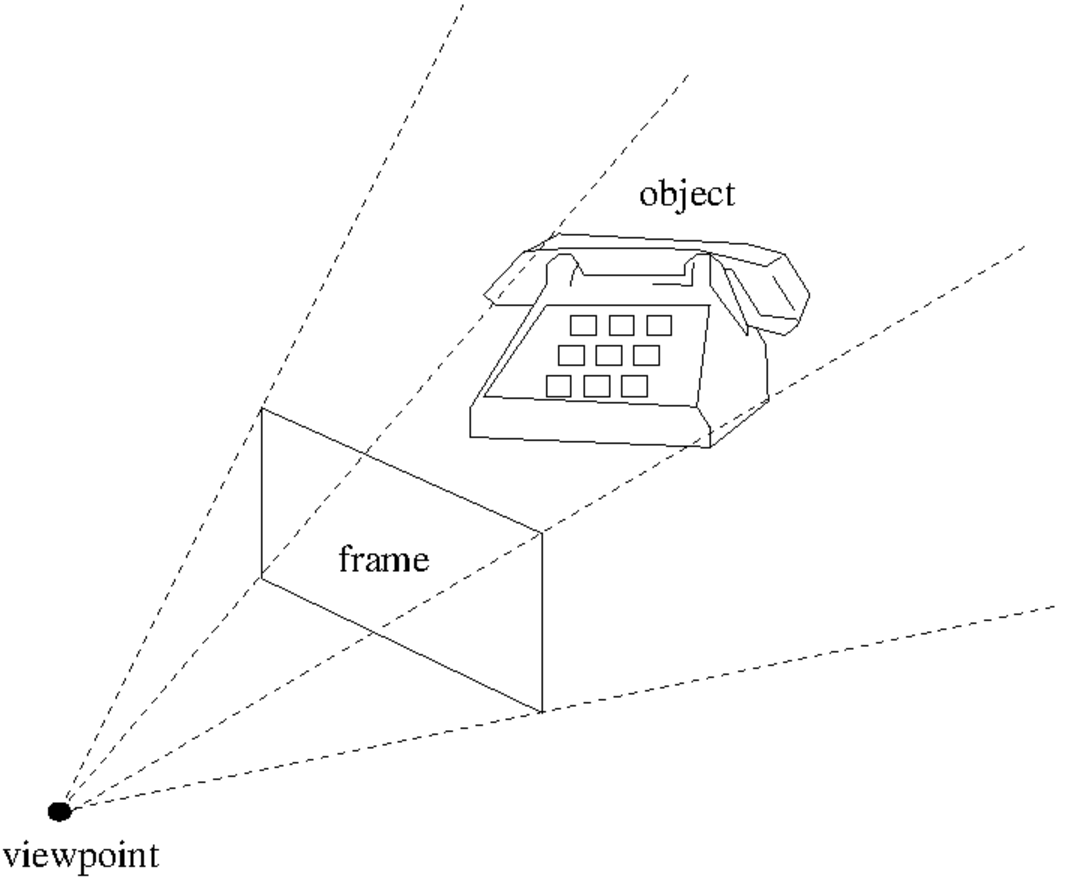
\includegraphics[width=2.3in, height=2in,angle = 0]{raytracing.pdf}
\end{center}
\end{figure}
Lines ('rays') are extended from the viewpoint through a dense grid of points on the window,
and checked for intersection with the object.  If such an intersection exists, it should be 
registered as a point on the object 'visible' from the viewpoint.  In computer graphics, these 
points are projected back on the window, which becomes a 2D image that can be displayed on the
computer screen.  For our purposes, we refrain from doing this projection, and store the 
full 3D coordinates of the detected point.\\
Note that a ray may intersect the object more than once.  In these cases, the intersection point
closest to the viewpoint is chosen, as the other points are 'hidden' by it.  As mentioned above,
there are two raytracing routines in this example program.  The robust routine calculates all
possible intersection points for each ray, and then choses the nearest one.  This should always
work, but can be slow since no information is re-used.  When we have found an intersection point
for a given ray, we can usually expect that the next, neighouring ray will intersect in a point
close to the one already found.  If this is the case, it would be speedier to use a local 
algorithm that converges on the intersection point quickly given a good initial guess.  This is
the basis for our 'quick' routine.  This routine uses the robust raytracing algorithm to find
the first point on a surface, and then it switches over to the fast method as long as it is 
possible to do so.  However, since the quick method never finds more than one intersection point,
and since a ray may generally intersect an object more than once, we have no guarantee that
the point found is the one truly visible from the viewpoint.  There are some checking procedures
that make things better, but we still have no guarantee.   If the user inspects the results 
obtained, he will notice this problem even on the simple example given here.  In general, it
can be said that the rapid algorithm should only be used in some special cases, where we know
for a fact that any ray from the viewpoint will not intersect the surface more than once.\\

This is the only of the example programs that can be run with a command line argument.  If the 
first argument is \verb/q/, then the quick raytracing routine will be invoked.  Else, the
robust and slow routine is used.

\subsubsection{What it demonstrates}
\begin{enumerate}
\item The basic setting and principe of a raytracer, with a defined viewpoint, window and 
intersection with rays.
\item The use of the SISL routine \verb/s1856/, which calculates all intersections between a 
spline surface and a line.
\item The use of the SISL routine \verb/s1518/, which converges to an intersection between
a spline surface and a line, given a good initial guess.
\end{enumerate}
\subsubsection{Input/output}
The surface to be raytraced is read from the file \verb/example10_surf.g2/, generated by
the \verb/example10/ program.  The other parameters necessary for the raytracing are hard-
coded (viewpoint, view window, resolution, etc.).  The resulting points are written to the
file \verb/example15_points.g2/. 

\chapter{The object viewer program}

\section{General}
The object viewer program bundled with this distribution of SISL is intended to be
a simple but handy tool for visualising curves and surfaces generated by SISL.  The
supported file format is the \verb/Go/ format, 
which is a simple, ASCII-based format defined by SINTEF.  The viewer is based on OpenGL.
An alternative viewer with a more evolved user interface, but also more dependencies can
be found in the library GoTools also provided by SINTEF Mathematics and Cybernetics.
The object(s) to be viewed are for this viewer specified on the command line when starting the 
program.  Once the program is started, the user cannot open other files containing
SISL objects.  The viewer allows the user to zoom, pan and rotate the objects with
the mouse, and some other useful commands can be accessed through the keyboard.
\\
\\
In the viewer window, several curves and surfaces can be displayed simultaneously.
At all times, exactly \emph{one} surface and \emph{one} curve are defined as being
\emph{active} (the other ones being \emph{passive}).  With keyboard commands, the user
can change the currently active surface/curve.  An object just becoming active will
flash for a few seconds.  With other keyboard commands, the user can \emph{enable/disable}
surfaces and curves.  This refers to turning the display of these objects on or off.
For details, refer to the section on keyboard commands.

\section{Compiling the viewer}
The default cmake setup is not to compile example programs, the stream library and the viewer.
To enable compilation of the example programs the cmake call must be extended with
-Dsisl\_COMPILE\_VIEWER=ON. This option also enables compilation of the streaming library.
With ccmake compile options are changed pressing enter. In cmake-gui compilation of the viewer
is invoked by ticking the appropriate box.
Compilation and linking is performed with the call
\begin{verbatim}
$ make sisl_view_demo
\end{verbatim}
The viewer is written in C++.

\section{Command line arguments}
When starting up the viewer, the options listed below can be used.  If no option is
specified, a short text listing the available options is printed on screen.

\begin{itemize}
\item[$\bullet$] \textbf{\protect \Verb/s/} \textit{filename} - view the surface(s) contained in
the file \textit{filename}.  Note: this command line option can be used repetitively if
the user wants to inspect several surfaces at once.
\item[$\bullet$] \textbf{\protect \Verb/c/} \textit{filename} - view the curve(s) contained in the
file \textit{filename}.  Note: this command can be used repetitively if the user wants
to inspect several curves at once.
\item[$\bullet$] \textbf{\protect \Verb/p/} \textit{filename} - view the point(s) contained in 
the file \textit{filename}.  Note: this command line option can be used repetitively if
the user wants to inspect several surfaces at once.
\item[$\bullet$] \textbf{\protect \Verb/r/} \textit{integer} set surface refinement factor 
(number of facets in each direction on the surface). Default value is 100.  Higher values
gives smoother drawing of the surface.  NB: this option has to \emph{precede} the 's' 
option!
\item[$\bullet$] \textbf{\protect \Verb/e/} \textit{string} the string contains keypresses to execute
directly upon start (see the section on keyboard control keys for details).
\item[$\bullet$] \textbf{\protect \Verb/hotkeys/} does not start the viewer, but displays a list 
of keyboard commands that can be used when viewing.
\end{itemize}

A file can contain one or several curves, or one or several surfaces.  Files containing
both curves and surfaces are not supported.  The viewer can read several files to be
viewed at once.  On the command line, each ``curve'' file should be preceded with the
letter 'c', and each ``surface'' file should be preceded with the letter 's'.  After 
launch, all the objects contained in the given files are shown simultaneously.  The user
can disable the view of certain curves and surfaces if he or she wants to.  

\section{User controls}

After program launch, the viewing of curves and surfaces can be controlled with the mouse
and keyboard.  The mouse is used to define viewing angle, direction and zoom factor, while
keyboard keys are used to turn on/off objects and to change certain view parameters.

\subsection{Mouse commands}
It is assumed that a 3-button mouse is used.  By dragging the mouse while holding down the
\emph{left button}, the user can rotate the current view in an intuitive way.  By dragging
with a certain speed, the view will continue to rotate even after the left button is released.
The \emph{middle button} is used for zooming.  Hold down this button and move the mouse 
forwards and backwards in order to zoom in and out.  Holding down the \emph{right button}
while dragging the mouse moves the view up and down.

\subsection{Keyboard commands}

The available keyboard commands are:

\begin{itemize}
\item[$\bullet$] \textbf{\protect \Verb/q/} - quit the viewer program
\item[$\bullet$] \textbf{\protect \Verb/<space>/} - change the currently active curve 
(cycles through each of them)
\item[$\bullet$] \textbf{\protect \Verb/<tab/} - change the currently active surface 
(cycles through each of them)
\item[$\bullet$] \textbf{\protect \Verb/w/} - turn on/off the wireframe display for surfaces
\item[$\bullet$] \textbf{\protect \Verb/B/} - toggle between black and white color for backgrounds
\item[$\bullet$] \textbf{\protect \Verb/A/} - toggle drawing of coordinate axes on/off
\item[$\bullet$] \textbf{\protect \Verb/S/} - toggle drawing of surfaces
\item[$\bullet$] \textbf{\protect \Verb/e/} - toggle visibility of currently active surface
\item[$\bullet$] \textbf{\protect \Verb/a/} - make all loaded surfaces visible
\item[$\bullet$] \textbf{\protect \Verb/d/} - hide all surfaces except the currently active one
\item[$\bullet$] \textbf{\protect \Verb/<ctrl>-e/} - toggle visibility of currently active curve
\item[$\bullet$] \textbf{\protect \Verb/<ctrl>-a/} - make all loaded curves visible
\item[$\bullet$] \textbf{\protect \Verb/<ctrl>-d/} - hide all curves except the currently active one
\item[$\bullet$] \textbf{\protect \Verb/O/} - center all objects around origo, and rescale objects
so that they fit inside the unit volume (does not preserve aspect ratio)
\item[$\bullet$] \textbf{\protect \Verb/o/} - center all objects around origo, no rescaling
\item[$\bullet$] \textbf{\protect \Verb/+/} - increase thickness of axes
\item[$\bullet$] \textbf{\protect \Verb/-/} - decrease thickness of axes
\item[$\bullet$] \textbf{\protect \Verb/>/} - increase size of points
\item[$\bullet$] \textbf{\protect \Verb/</} - decrease size of points
\item[$\bullet$] \textbf{\protect \Verb///} - decrease length of axes
\item[$\bullet$] \textbf{\protect \Verb/<esc>-w-[n]/} - store viewpoint in slot [n], where [n]
is a number from 0 to 9.  The viewpoint will be saved to file, and can such be preserved
from one session to another.
\item[$\bullet$] \textbf{\protect \Verb/<esc>-r-[n]/} - load a previously saved viewpoint from
slot [n], where [n] is a number from 0 to 9.
\end{itemize}

\cleardoublepage
\input{chap_error_codes}
\cleardoublepage
\appendix


\chapter{GNU AFFERO GENERAL PUBLIC LICENSE}

\begin{center}
{\parindent 0in
  Version 3, 19 November 2007
  
Copyright \copyright\  2007 Free Software Foundation, Inc. \texttt{https://fsf.org/}

\bigskip
Everyone is permitted to copy and distribute verbatim copies of this

license document, but changing it is not allowed.}

\end{center}

\renewcommand{\abstractname}{Preamble}
\begin{abstract}
The GNU Affero General Public License is a free, copyleft license
for software and other kinds of works, specifically designed to ensure
cooperation with the community in the case of network server software.

The licenses for most software and other practical works are
designed to take away your freedom to share and change the works.  By
contrast, our General Public Licenses are intended to guarantee your
freedom to share and change all versions of a program--to make sure it
remains free software for all its users.

When we speak of free software, we are referring to freedom, not
price.  Our General Public Licenses are designed to make sure that you
have the freedom to distribute copies of free software (and charge for
them if you wish), that you receive source code or can get it if you
want it, that you can change the software or use pieces of it in new
free programs, and that you know you can do these things.

Developers that use our General Public Licenses protect your rights
with two steps: (1) assert copyright on the software, and (2) offer
you this License which gives you legal permission to copy, distribute
and/or modify the software.

A secondary benefit of defending all users' freedom is that
improvements made in alternate versions of the program, if they
receive widespread use, become available for other developers to
incorporate.  Many developers of free software are heartened and
encouraged by the resulting cooperation.  However, in the case of
software used on network servers, this result may fail to come about.
The GNU General Public License permits making a modified version and
letting the public access it on a server without ever releasing its
source code to the public.

The GNU Affero General Public License is designed specifically to
ensure that, in such cases, the modified source code becomes available
to the community.  It requires the operator of a network server to
provide the source code of the modified version running there to the
users of that server.  Therefore, public use of a modified version, on
a publicly accessible server, gives the public access to the source
code of the modified version.

An older license, called the Affero General Public License and
published by Affero, was designed to accomplish similar goals.  This is
a different license, not a version of the Affero GPL, but Affero has
released a new version of the Affero GPL which permits relicensing under
this license.

The precise terms and conditions for copying, distribution and
modification follow.
\end{abstract}

\begin{center}
{\Large \sc Terms and Conditions}
\end{center}


\begin{enumerate}

\addtocounter{enumi}{-1}

\item Definitions.

``This License'' refers to version 3 of the GNU Affero General Public License.

``Copyright'' also means copyright-like laws that apply to other kinds of
works, such as semiconductor masks.

``The Program'' refers to any copyrightable work licensed under this
License.  Each licensee is addressed as ``you''.  ``Licensees'' and
``recipients'' may be individuals or organizations.

To ``modify'' a work means to copy from or adapt all or part of the work
in a fashion requiring copyright permission, other than the making of an
exact copy.  The resulting work is called a ``modified version'' of the
earlier work or a work ``based on'' the earlier work.

A ``covered work'' means either the unmodified Program or a work based
on the Program.

To ``propagate'' a work means to do anything with it that, without
permission, would make you directly or secondarily liable for
infringement under applicable copyright law, except executing it on a
computer or modifying a private copy.  Propagation includes copying,
distribution (with or without modification), making available to the
public, and in some countries other activities as well.

To ``convey'' a work means any kind of propagation that enables other
parties to make or receive copies.  Mere interaction with a user through
a computer network, with no transfer of a copy, is not conveying.

An interactive user interface displays ``Appropriate Legal Notices''
to the extent that it includes a convenient and prominently visible
feature that (1) displays an appropriate copyright notice, and (2)
tells the user that there is no warranty for the work (except to the
extent that warranties are provided), that licensees may convey the
work under this License, and how to view a copy of this License.  If
the interface presents a list of user commands or options, such as a
menu, a prominent item in the list meets this criterion.

\item Source Code.

The ``source code'' for a work means the preferred form of the work
for making modifications to it.  ``Object code'' means any non-source
form of a work.

A ``Standard Interface'' means an interface that either is an official
standard defined by a recognized standards body, or, in the case of
interfaces specified for a particular programming language, one that
is widely used among developers working in that language.

The ``System Libraries'' of an executable work include anything, other
than the work as a whole, that (a) is included in the normal form of
packaging a Major Component, but which is not part of that Major
Component, and (b) serves only to enable use of the work with that
Major Component, or to implement a Standard Interface for which an
implementation is available to the public in source code form.  A
``Major Component'', in this context, means a major essential component
(kernel, window system, and so on) of the specific operating system
(if any) on which the executable work runs, or a compiler used to
produce the work, or an object code interpreter used to run it.

The ``Corresponding Source'' for a work in object code form means all
the source code needed to generate, install, and (for an executable
work) run the object code and to modify the work, including scripts to
control those activities.  However, it does not include the work's
System Libraries, or general-purpose tools or generally available free
programs which are used unmodified in performing those activities but
which are not part of the work.  For example, Corresponding Source
includes interface definition files associated with source files for
the work, and the source code for shared libraries and dynamically
linked subprograms that the work is specifically designed to require,
such as by intimate data communication or control flow between those
subprograms and other parts of the work.

The Corresponding Source need not include anything that users
can regenerate automatically from other parts of the Corresponding
Source.

The Corresponding Source for a work in source code form is that
same work.

\item Basic Permissions.

All rights granted under this License are granted for the term of
copyright on the Program, and are irrevocable provided the stated
conditions are met.  This License explicitly affirms your unlimited
permission to run the unmodified Program.  The output from running a
covered work is covered by this License only if the output, given its
content, constitutes a covered work.  This License acknowledges your
rights of fair use or other equivalent, as provided by copyright law.

You may make, run and propagate covered works that you do not
convey, without conditions so long as your license otherwise remains
in force.  You may convey covered works to others for the sole purpose
of having them make modifications exclusively for you, or provide you
with facilities for running those works, provided that you comply with
the terms of this License in conveying all material for which you do
not control copyright.  Those thus making or running the covered works
for you must do so exclusively on your behalf, under your direction
and control, on terms that prohibit them from making any copies of
your copyrighted material outside their relationship with you.

Conveying under any other circumstances is permitted solely under
the conditions stated below.  Sublicensing is not allowed; section 10
makes it unnecessary.

\item Protecting Users' Legal Rights From Anti-Circumvention Law.

No covered work shall be deemed part of an effective technological
measure under any applicable law fulfilling obligations under article
11 of the WIPO copyright treaty adopted on 20 December 1996, or
similar laws prohibiting or restricting circumvention of such
measures.

When you convey a covered work, you waive any legal power to forbid
circumvention of technological measures to the extent such circumvention
is effected by exercising rights under this License with respect to
the covered work, and you disclaim any intention to limit operation or
modification of the work as a means of enforcing, against the work's
users, your or third parties' legal rights to forbid circumvention of
technological measures.

\item Conveying Verbatim Copies.

You may convey verbatim copies of the Program's source code as you
receive it, in any medium, provided that you conspicuously and
appropriately publish on each copy an appropriate copyright notice;
keep intact all notices stating that this License and any
non-permissive terms added in accord with section 7 apply to the code;
keep intact all notices of the absence of any warranty; and give all
recipients a copy of this License along with the Program.

You may charge any price or no price for each copy that you convey,
and you may offer support or warranty protection for a fee.

\item Conveying Modified Source Versions.

You may convey a work based on the Program, or the modifications to
produce it from the Program, in the form of source code under the
terms of section 4, provided that you also meet all of these conditions:
  \begin{enumerate}
  \item The work must carry prominent notices stating that you modified
  it, and giving a relevant date.

  \item The work must carry prominent notices stating that it is
  released under this License and any conditions added under section
  7.  This requirement modifies the requirement in section 4 to
  ``keep intact all notices''.

  \item You must license the entire work, as a whole, under this
  License to anyone who comes into possession of a copy.  This
  License will therefore apply, along with any applicable section 7
  additional terms, to the whole of the work, and all its parts,
  regardless of how they are packaged.  This License gives no
  permission to license the work in any other way, but it does not
  invalidate such permission if you have separately received it.

  \item If the work has interactive user interfaces, each must display
  Appropriate Legal Notices; however, if the Program has interactive
  interfaces that do not display Appropriate Legal Notices, your
  work need not make them do so.
\end{enumerate}
A compilation of a covered work with other separate and independent
works, which are not by their nature extensions of the covered work,
and which are not combined with it such as to form a larger program,
in or on a volume of a storage or distribution medium, is called an
``aggregate'' if the compilation and its resulting copyright are not
used to limit the access or legal rights of the compilation's users
beyond what the individual works permit.  Inclusion of a covered work
in an aggregate does not cause this License to apply to the other
parts of the aggregate.

\item Conveying Non-Source Forms.

You may convey a covered work in object code form under the terms
of sections 4 and 5, provided that you also convey the
machine-readable Corresponding Source under the terms of this License,
in one of these ways:
  \begin{enumerate}
  \item Convey the object code in, or embodied in, a physical product
  (including a physical distribution medium), accompanied by the
  Corresponding Source fixed on a durable physical medium
  customarily used for software interchange.

  \item Convey the object code in, or embodied in, a physical product
  (including a physical distribution medium), accompanied by a
  written offer, valid for at least three years and valid for as
  long as you offer spare parts or customer support for that product
  model, to give anyone who possesses the object code either (1) a
  copy of the Corresponding Source for all the software in the
  product that is covered by this License, on a durable physical
  medium customarily used for software interchange, for a price no
  more than your reasonable cost of physically performing this
  conveying of source, or (2) access to copy the
  Corresponding Source from a network server at no charge.

  \item Convey individual copies of the object code with a copy of the
  written offer to provide the Corresponding Source.  This
  alternative is allowed only occasionally and noncommercially, and
  only if you received the object code with such an offer, in accord
  with subsection 6b.

  \item Convey the object code by offering access from a designated
  place (gratis or for a charge), and offer equivalent access to the
  Corresponding Source in the same way through the same place at no
  further charge.  You need not require recipients to copy the
  Corresponding Source along with the object code.  If the place to
  copy the object code is a network server, the Corresponding Source
  may be on a different server (operated by you or a third party)
  that supports equivalent copying facilities, provided you maintain
  clear directions next to the object code saying where to find the
  Corresponding Source.  Regardless of what server hosts the
  Corresponding Source, you remain obligated to ensure that it is
  available for as long as needed to satisfy these requirements.

  \item Convey the object code using peer-to-peer transmission, provided
  you inform other peers where the object code and Corresponding
  Source of the work are being offered to the general public at no
  charge under subsection 6d.
  \end{enumerate}

A separable portion of the object code, whose source code is excluded
from the Corresponding Source as a System Library, need not be
included in conveying the object code work.

A ``User Product'' is either (1) a ``consumer product'', which means any
tangible personal property which is normally used for personal, family,
or household purposes, or (2) anything designed or sold for incorporation
into a dwelling.  In determining whether a product is a consumer product,
doubtful cases shall be resolved in favor of coverage.  For a particular
product received by a particular user, ``normally used'' refers to a
typical or common use of that class of product, regardless of the status
of the particular user or of the way in which the particular user
actually uses, or expects or is expected to use, the product.  A product
is a consumer product regardless of whether the product has substantial
commercial, industrial or non-consumer uses, unless such uses represent
the only significant mode of use of the product.

``Installation Information'' for a User Product means any methods,
procedures, authorization keys, or other information required to install
and execute modified versions of a covered work in that User Product from
a modified version of its Corresponding Source.  The information must
suffice to ensure that the continued functioning of the modified object
code is in no case prevented or interfered with solely because
modification has been made.

If you convey an object code work under this section in, or with, or
specifically for use in, a User Product, and the conveying occurs as
part of a transaction in which the right of possession and use of the
User Product is transferred to the recipient in perpetuity or for a
fixed term (regardless of how the transaction is characterized), the
Corresponding Source conveyed under this section must be accompanied
by the Installation Information.  But this requirement does not apply
if neither you nor any third party retains the ability to install
modified object code on the User Product (for example, the work has
been installed in ROM).

The requirement to provide Installation Information does not include a
requirement to continue to provide support service, warranty, or updates
for a work that has been modified or installed by the recipient, or for
the User Product in which it has been modified or installed.  Access to a
network may be denied when the modification itself materially and
adversely affects the operation of the network or violates the rules and
protocols for communication across the network.

Corresponding Source conveyed, and Installation Information provided,
in accord with this section must be in a format that is publicly
documented (and with an implementation available to the public in
source code form), and must require no special password or key for
unpacking, reading or copying.

\item Additional Terms.

``Additional permissions'' are terms that supplement the terms of this
License by making exceptions from one or more of its conditions.
Additional permissions that are applicable to the entire Program shall
be treated as though they were included in this License, to the extent
that they are valid under applicable law.  If additional permissions
apply only to part of the Program, that part may be used separately
under those permissions, but the entire Program remains governed by
this License without regard to the additional permissions.

When you convey a copy of a covered work, you may at your option
remove any additional permissions from that copy, or from any part of
it.  (Additional permissions may be written to require their own
removal in certain cases when you modify the work.)  You may place
additional permissions on material, added by you to a covered work,
for which you have or can give appropriate copyright permission.

Notwithstanding any other provision of this License, for material you
add to a covered work, you may (if authorized by the copyright holders of
that material) supplement the terms of this License with terms:
  \begin{enumerate}
  \item Disclaiming warranty or limiting liability differently from the
  terms of sections 15 and 16 of this License; or

  \item Requiring preservation of specified reasonable legal notices or
  author attributions in that material or in the Appropriate Legal
  Notices displayed by works containing it; or

  \item Prohibiting misrepresentation of the origin of that material, or
  requiring that modified versions of such material be marked in
  reasonable ways as different from the original version; or

  \item Limiting the use for publicity purposes of names of licensors or
  authors of the material; or

  \item Declining to grant rights under trademark law for use of some
  trade names, trademarks, or service marks; or

  \item Requiring indemnification of licensors and authors of that
  material by anyone who conveys the material (or modified versions of
  it) with contractual assumptions of liability to the recipient, for
  any liability that these contractual assumptions directly impose on
  those licensors and authors.
  \end{enumerate}

All other non-permissive additional terms are considered ``further
restrictions'' within the meaning of section 10.  If the Program as you
received it, or any part of it, contains a notice stating that it is
governed by this License along with a term that is a further
restriction, you may remove that term.  If a license document contains
a further restriction but permits relicensing or conveying under this
License, you may add to a covered work material governed by the terms
of that license document, provided that the further restriction does
not survive such relicensing or conveying.

If you add terms to a covered work in accord with this section, you
must place, in the relevant source files, a statement of the
additional terms that apply to those files, or a notice indicating
where to find the applicable terms.

Additional terms, permissive or non-permissive, may be stated in the
form of a separately written license, or stated as exceptions;
the above requirements apply either way.

\item Termination.

You may not propagate or modify a covered work except as expressly
provided under this License.  Any attempt otherwise to propagate or
modify it is void, and will automatically terminate your rights under
this License (including any patent licenses granted under the third
paragraph of section 11).

However, if you cease all violation of this License, then your
license from a particular copyright holder is reinstated (a)
provisionally, unless and until the copyright holder explicitly and
finally terminates your license, and (b) permanently, if the copyright
holder fails to notify you of the violation by some reasonable means
prior to 60 days after the cessation.

Moreover, your license from a particular copyright holder is
reinstated permanently if the copyright holder notifies you of the
violation by some reasonable means, this is the first time you have
received notice of violation of this License (for any work) from that
copyright holder, and you cure the violation prior to 30 days after
your receipt of the notice.

Termination of your rights under this section does not terminate the
licenses of parties who have received copies or rights from you under
this License.  If your rights have been terminated and not permanently
reinstated, you do not qualify to receive new licenses for the same
material under section 10.

\item Acceptance Not Required for Having Copies.

You are not required to accept this License in order to receive or
run a copy of the Program.  Ancillary propagation of a covered work
occurring solely as a consequence of using peer-to-peer transmission
to receive a copy likewise does not require acceptance.  However,
nothing other than this License grants you permission to propagate or
modify any covered work.  These actions infringe copyright if you do
not accept this License.  Therefore, by modifying or propagating a
covered work, you indicate your acceptance of this License to do so.

\item Automatic Licensing of Downstream Recipients.

Each time you convey a covered work, the recipient automatically
receives a license from the original licensors, to run, modify and
propagate that work, subject to this License.  You are not responsible
for enforcing compliance by third parties with this License.

An ``entity transaction'' is a transaction transferring control of an
organization, or substantially all assets of one, or subdividing an
organization, or merging organizations.  If propagation of a covered
work results from an entity transaction, each party to that
transaction who receives a copy of the work also receives whatever
licenses to the work the party's predecessor in interest had or could
give under the previous paragraph, plus a right to possession of the
Corresponding Source of the work from the predecessor in interest, if
the predecessor has it or can get it with reasonable efforts.

You may not impose any further restrictions on the exercise of the
rights granted or affirmed under this License.  For example, you may
not impose a license fee, royalty, or other charge for exercise of
rights granted under this License, and you may not initiate litigation
(including a cross-claim or counterclaim in a lawsuit) alleging that
any patent claim is infringed by making, using, selling, offering for
sale, or importing the Program or any portion of it.

\item Patents.

A ``contributor'' is a copyright holder who authorizes use under this
License of the Program or a work on which the Program is based.  The
work thus licensed is called the contributor's ``contributor version''.

A contributor's ``essential patent claims'' are all patent claims
owned or controlled by the contributor, whether already acquired or
hereafter acquired, that would be infringed by some manner, permitted
by this License, of making, using, or selling its contributor version,
but do not include claims that would be infringed only as a
consequence of further modification of the contributor version.  For
purposes of this definition, ``control'' includes the right to grant
patent sublicenses in a manner consistent with the requirements of
this License.

Each contributor grants you a non-exclusive, worldwide, royalty-free
patent license under the contributor's essential patent claims, to
make, use, sell, offer for sale, import and otherwise run, modify and
propagate the contents of its contributor version.

In the following three paragraphs, a ``patent license'' is any express
agreement or commitment, however denominated, not to enforce a patent
(such as an express permission to practice a patent or covenant not to
sue for patent infringement).  To ``grant'' such a patent license to a
party means to make such an agreement or commitment not to enforce a
patent against the party.

If you convey a covered work, knowingly relying on a patent license,
and the Corresponding Source of the work is not available for anyone
to copy, free of charge and under the terms of this License, through a
publicly available network server or other readily accessible means,
then you must either (1) cause the Corresponding Source to be so
available, or (2) arrange to deprive yourself of the benefit of the
patent license for this particular work, or (3) arrange, in a manner
consistent with the requirements of this License, to extend the patent
license to downstream recipients.  ``Knowingly relying'' means you have
actual knowledge that, but for the patent license, your conveying the
covered work in a country, or your recipient's use of the covered work
in a country, would infringe one or more identifiable patents in that
country that you have reason to believe are valid.

If, pursuant to or in connection with a single transaction or
arrangement, you convey, or propagate by procuring conveyance of, a
covered work, and grant a patent license to some of the parties
receiving the covered work authorizing them to use, propagate, modify
or convey a specific copy of the covered work, then the patent license
you grant is automatically extended to all recipients of the covered
work and works based on it.

A patent license is ``discriminatory'' if it does not include within
the scope of its coverage, prohibits the exercise of, or is
conditioned on the non-exercise of one or more of the rights that are
specifically granted under this License.  You may not convey a covered
work if you are a party to an arrangement with a third party that is
in the business of distributing software, under which you make payment
to the third party based on the extent of your activity of conveying
the work, and under which the third party grants, to any of the
parties who would receive the covered work from you, a discriminatory
patent license (a) in connection with copies of the covered work
conveyed by you (or copies made from those copies), or (b) primarily
for and in connection with specific products or compilations that
contain the covered work, unless you entered into that arrangement,
or that patent license was granted, prior to 28 March 2007.

Nothing in this License shall be construed as excluding or limiting
any implied license or other defenses to infringement that may
otherwise be available to you under applicable patent law.

\item No Surrender of Others' Freedom.

If conditions are imposed on you (whether by court order, agreement or
otherwise) that contradict the conditions of this License, they do not
excuse you from the conditions of this License.  If you cannot convey a
covered work so as to satisfy simultaneously your obligations under this
License and any other pertinent obligations, then as a consequence you may
not convey it at all.  For example, if you agree to terms that obligate you
to collect a royalty for further conveying from those to whom you convey
the Program, the only way you could satisfy both those terms and this
License would be to refrain entirely from conveying the Program.

\item Remote Network Interaction; Use with the GNU General Public License.

Notwithstanding any other provision of this License, if you modify the
Program, your modified version must prominently offer all users interacting
with it remotely through a computer network (if your version supports such
interaction) an opportunity to receive the Corresponding Source of your
version by providing access to the Corresponding Source from a network
server at no charge, through some standard or customary means of
facilitating copying of software.  This Corresponding Source shall include
the Corresponding Source for any work covered by version 3 of the GNU
General Public License that is incorporated pursuant to the following
paragraph.

Notwithstanding any other provision of this License, you have permission to
link or combine any covered work with a work licensed under version 3 of
the GNU General Public License into a single combined work, and to convey
the resulting work.  The terms of this License will continue to apply to
the part which is the covered work, but the work with which it is combined
will remain governed by version 3 of the GNU General Public License.

\item Revised Versions of this License.

The Free Software Foundation may publish revised and/or new versions of
the GNU Affero General Public License from time to time.  Such new versions will
be similar in spirit to the present version, but may differ in detail to
address new problems or concerns.

Each version is given a distinguishing version number.  If the
Program specifies that a certain numbered version of the GNU Affero General
Public License ``or any later version'' applies to it, you have the
option of following the terms and conditions either of that numbered
version or of any later version published by the Free Software
Foundation.  If the Program does not specify a version number of the
GNU Affero General Public License, you may choose any version ever published
by the Free Software Foundation.

If the Program specifies that a proxy can decide which future
versions of the GNU Affero General Public License can be used, that proxy's
public statement of acceptance of a version permanently authorizes you
to choose that version for the Program.

Later license versions may give you additional or different
permissions.  However, no additional obligations are imposed on any
author or copyright holder as a result of your choosing to follow a
later version.

\item Disclaimer of Warranty.

\begin{sloppypar}
 THERE IS NO WARRANTY FOR THE PROGRAM, TO THE EXTENT PERMITTED BY
 APPLICABLE LAW.  EXCEPT WHEN OTHERWISE STATED IN WRITING THE
 COPYRIGHT HOLDERS AND/OR OTHER PARTIES PROVIDE THE PROGRAM ``AS IS''
 WITHOUT WARRANTY OF ANY KIND, EITHER EXPRESSED OR IMPLIED,
 INCLUDING, BUT NOT LIMITED TO, THE IMPLIED WARRANTIES OF
 MERCHANTABILITY AND FITNESS FOR A PARTICULAR PURPOSE.  THE ENTIRE
 RISK AS TO THE QUALITY AND PERFORMANCE OF THE PROGRAM IS WITH YOU.
 SHOULD THE PROGRAM PROVE DEFECTIVE, YOU ASSUME THE COST OF ALL
 NECESSARY SERVICING, REPAIR OR CORRECTION.
\end{sloppypar}

\item Limitation of Liability.

 IN NO EVENT UNLESS REQUIRED BY APPLICABLE LAW OR AGREED TO IN
 WRITING WILL ANY COPYRIGHT HOLDER, OR ANY OTHER PARTY WHO MODIFIES
 AND/OR CONVEYS THE PROGRAM AS PERMITTED ABOVE, BE LIABLE TO YOU FOR
 DAMAGES, INCLUDING ANY GENERAL, SPECIAL, INCIDENTAL OR CONSEQUENTIAL
 DAMAGES ARISING OUT OF THE USE OR INABILITY TO USE THE PROGRAM
 (INCLUDING BUT NOT LIMITED TO LOSS OF DATA OR DATA BEING RENDERED
 INACCURATE OR LOSSES SUSTAINED BY YOU OR THIRD PARTIES OR A FAILURE
 OF THE PROGRAM TO OPERATE WITH ANY OTHER PROGRAMS), EVEN IF SUCH
 HOLDER OR OTHER PARTY HAS BEEN ADVISED OF THE POSSIBILITY OF SUCH
 DAMAGES.

\item Interpretation of Sections 15 and 16.

If the disclaimer of warranty and limitation of liability provided
above cannot be given local legal effect according to their terms,
reviewing courts shall apply local law that most closely approximates
an absolute waiver of all civil liability in connection with the
Program, unless a warranty or assumption of liability accompanies a
copy of the Program in return for a fee.

\begin{center}
{\Large\sc End of Terms and Conditions}
\end{center}
\pagebreak[2]

\section*{Appendix: How to Apply These Terms to Your New Programs}

If you develop a new program, and you want it to be of the greatest
possible use to the public, the best way to achieve this is to make it
free software which everyone can redistribute and change under these terms.

To do so, attach the following notices to the program.  It is safest
to attach them to the start of each source file to most effectively
state the exclusion of warranty; and each file should have at least
the ``copyright'' line and a pointer to where the full notice is found.

{\footnotesize
\begin{verbatim}
<one line to give the program's name and a brief idea of what it does.>

Copyright (C) <textyear>  <name of author>

This program is free software: you can redistribute it and/or modify
it under the terms of the GNU Affero General Public License as published by
the Free Software Foundation, either version 3 of the License, or
(at your option) any later version.

This program is distributed in the hope that it will be useful,
but WITHOUT ANY WARRANTY; without even the implied warranty of
MERCHANTABILITY or FITNESS FOR A PARTICULAR PURPOSE.  See the
GNU Affero General Public License for more details.

You should have received a copy of the GNU Affero General Public License
along with this program.  If not, see <https://www.gnu.org/licenses/>.
\end{verbatim}
}

Also add information on how to contact you by electronic and paper mail.

If your software can interact with users remotely through a computer
network, you should also make sure that it provides a way for users to
get its source.  For example, if your program is a web application, its
interface could display a ``Source'' link that leads users to an archive
of the code.  There are many ways you could offer source, and different
solutions will be better for different programs; see section 13 for the
specific requirements.

You should also get your employer (if you work as a programmer) or
school, if any, to sign a ``copyright disclaimer'' for the program, if
necessary.  For more information on this, and how to apply and follow
the GNU AGPL, see \texttt{https://www.gnu.org/licenses/}.

\end{enumerate}

\end{document}

%%% Local Variables:
%%% mode: latex
%%% TeX-master: t
%%% End:


\cleardoublepage
\printindex
\end{document}
